\documentclass[11pt, a4paper]{article}
%\usepackage{proj1}
\usepackage{natbib}
\usepackage{fancyhdr}  
\usepackage{subcaption}
\usepackage{caption}
\usepackage{graphicx}
\usepackage[autolanguage,nosepfour]{numprint}
\usepackage{multirow}
\linespread{1.25} 
\setlength{\parindent}{0cm}
\graphicspath{{Images/}}
\usepackage{hyperref}
\usepackage{amsmath}
\usepackage{amsfonts}
\usepackage{amssymb}
\usepackage{amsthm}
\usepackage{mathtools}
\usepackage{commath}
\usepackage{bbm}
\usepackage[ruled,vlined]{algorithm2e}

%\usepackage[sc,osf]{mathpazo}
\usepackage{subcaption}
\usepackage[a4paper, top=1in, left=1.0in, right=1.0in, bottom=1in, includehead, includefoot]{geometry} %Usually have top as 1in

\usepackage{listings}
\usepackage{color} %red, green, blue, yellow, cyan, magenta, black, white
\definecolor{mygreen}{RGB}{28,172,0} % color values Red, Green, Blue
\definecolor{mylilas}{RGB}{170,55,241}


\hypersetup{colorlinks,linkcolor={black},citecolor={blue},urlcolor={black}}
\usepackage{color}
\urlstyle{same}


\theoremstyle{definition}
\newtheorem{definition}{Definition}[section]

\newcommand{\adja}{q_a}
\newcommand{\adjb}{q_b}
\newcommand{\adjaB}{q_{a,\partial \Omega}}
\newcommand{\adjbB}{q_{b,\partial \Omega}}
\newcommand{\adjB}{q_{\partial \Omega}}
\newcommand{\Adja}{\mathbf{p}}
\newcommand{\Adjb}{q}
\newcommand{\adj}{q}
\newcommand{\Adjc}{{q}_{\partial \Omega}}
\newcommand{\ra}{\rho_a}
\newcommand{\rb}{\rho_b}
\newcommand{\w}{\mathbf{w}}
\newcommand{\f}{\mathbf{f}}
\newcommand{\ve}{\mathbf{v}}
\newcommand{\n}{\mathbf{n}}
\newcommand{\h}{\mathbf{h}}
\newcommand{\K}{\mathbf{K}}
\newcommand{\hr}{\widehat \rho}
\newcommand{\jf}{\mathbf j}

\DeclareMathOperator{\sgn}{sgn}
\DeclareMathOperator{\Grad}{Grad}
\DeclareMathOperator{\Div}{Div}
\DeclareMathOperator{\Lap}{Lap}



\title{{\huge Annual Review \\ PDE-Constrained Optimization \\for Multiscale Particle Dynamics} \\ with Industrial Applications}
\author{Jonna C. Roden\\ \\Supervision by Dr Ben Goddard and Dr John Pearson\\ \vspace{0.5cm} Maxwell Institute Graduate School for Analysis and its Applications}
\date{\today}


\pagenumbering{gobble}
\begin{document}
	\maketitle
	
	\newpage
	%\section*{Acknowledgements}
	%+ Later +
	%\newpage
	\pagenumbering{Roman} 
	\tableofcontents
	%\newpage
	%\listoffigures
	%\listoftables
	\newpage
	\pagenumbering{arabic} 
	
	\section{Introduction}
	At the point of the second year review, a good point was reached to develop both the models and the numerical methods further towards eventual industrial applications. 
	At first, the implementation of the inertial equations, which were derived in the second year report, has been completed, and a few representative 1D examples were developed.\\
	\\
	A large part of the efforts during this year has been put into the development of the 'MultiShape' implementation for PDE-constrained optimization problems. This is a spectral element method, which can be seen as an extension to the pseudospectral methods we have been using throughout this work.\\
	Mention these in intro:
	\begin{itemize}
	\item Sparse to Fine Grid Stuff
	\item Final time target derivation
	\item Averaging 3D to 2D
	\item Flow around Constriction
	\item Inertial Equations Examples
	\item Multiple Species (tbc) Optimality Conditions
	\end{itemize}
	
	\section{Multishape Implementation}
	\documentclass[11pt, a4paper]{article}
%\usepackage{proj1}
\usepackage{natbib}
\usepackage{fancyhdr}  
\usepackage{subcaption}
\usepackage{caption}
\usepackage{graphicx}
\usepackage{numprint}
\usepackage{multirow}
\linespread{1.25} 
\setlength{\parindent}{0cm}
\graphicspath{{Images/}}
\usepackage{hyperref}
\usepackage{amsmath}
\usepackage{amsfonts}
\usepackage{amssymb}
\usepackage{amsthm}
\usepackage{mathtools}
\usepackage{commath}
\usepackage{bbm}

%\usepackage[sc,osf]{mathpazo}
\usepackage{subcaption}
\usepackage[a4paper, top=1in, left=1.0in, right=1.0in, bottom=1in, includehead, includefoot]{geometry} %Usually have top as 1in

\usepackage{listings}
\usepackage{color} %red, green, blue, yellow, cyan, magenta, black, white
\definecolor{mygreen}{RGB}{28,172,0} % color values Red, Green, Blue
\definecolor{mylilas}{RGB}{170,55,241}


\hypersetup{colorlinks,linkcolor={black},citecolor={blue},urlcolor={black}}
\usepackage{color}
\urlstyle{same}


\theoremstyle{definition}
\newtheorem{definition}{Definition}[section]

\newcommand{\adja}{q_a}
\newcommand{\adjb}{q_b}
\newcommand{\adjaB}{q_{a,\partial \Omega}}
\newcommand{\adjbB}{q_{b,\partial \Omega}}
\newcommand{\adjB}{q_{\partial \Omega}}
\newcommand{\Adja}{\mathbf{p}}
\newcommand{\Adjb}{q}
\newcommand{\adj}{q}
\newcommand{\Adjc}{{q}_{\partial \Omega}}
\newcommand{\ra}{\rho_a}
\newcommand{\rb}{\rho_b}
\newcommand{\w}{\mathbf{w}}
\newcommand{\f}{\mathbf{f}}
\newcommand{\ve}{\mathbf{v}}
\newcommand{\n}{\mathbf{n}}
\newcommand{\h}{\mathbf{h}}
\newcommand{\K}{\mathbf{K}}
\newcommand{\hr}{\widehat \rho}
\newcommand{\jf}{\mathbf j}

%	\begin{figure}[h]
%		\centering
%		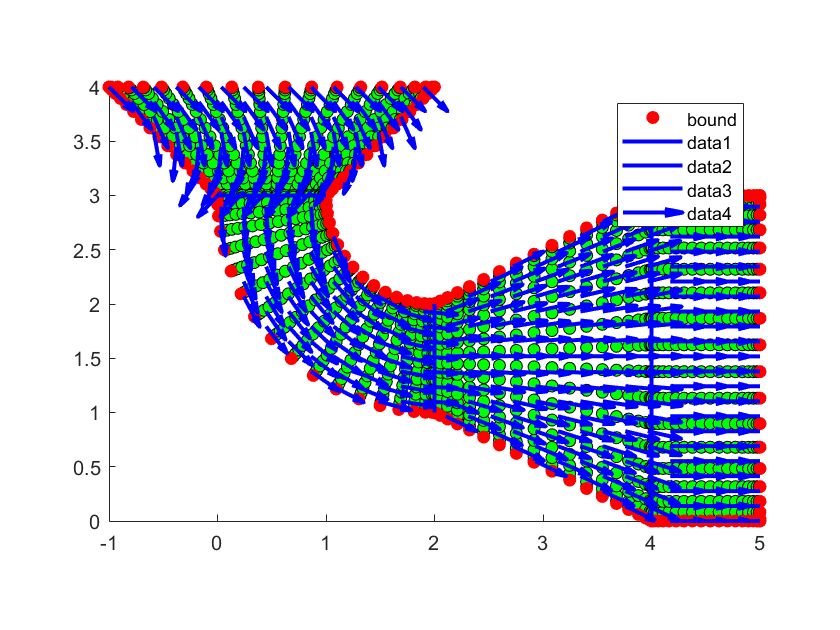
\includegraphics[scale=0.35]{F1.png}
%		\caption{Forward $\rho$ for $a = 0.01$} 
%		\label{F1}
%	\end{figure}

\begin{document}
\section*{MultiShape Theory}
The code library 2DChebClass, introduced in \cite{GoddardPseudospectralCode1}, is a tool for solving PDEs using pseudospectral methods in one and two dimensions on different domains, such as quadrilaterals, wedges and periodic boxes. The aim of this library is to provide a toolbox for solving DDFT in an efficient and user-friendly manner. This includes the automatic set-up of differentiation and convolution matrices, interpolation and integration vectors, as well as domain discretization using pseudospectral methods, identification of boundaries and application of boundary conditions. The library's features are thoroughly explained in \cite{GoddardPseudospectralCode1}.
\\
While the library supports solutions to PDEs on various single shapes, the method is now extended to compute the solution to a PDE on a complex domain, or multishape, which is composed of a number of quadrilaterals and wedges. The philosophy of this multishape code is to use the existing code library \cite{GoddardPseudospectralCode1}, which is designed to efficiently and accurately solve PDEs on individual shapes, to do the same on a multishape with minimal additional effort. 
\\
\\
The solution of a PDE on such a multishape domain is achieved by employing the spectral element method (SEM), by thinking of each of the shapes as the discretization elements of SEM.
This method is similar to the finite element method (FEM). FEM discretizes a domain into elements and computes the solution to a given PDE on each of those elements. Expansions of basis functions are used, which are low order polynomials, for interpolation on an equispaced grid. SEM follows the same philosophy but uses higher order basis functions such as Chebyshev or Lagrange polynomials and Chebyshev-Lobatto points on the interpolation grid on each element, as opposed to an equispaced grid, to avoid the Runge phenomenon. At the intersections between the elements, $C^0$ continuity is enforced. SEM was first introduced by Patera \cite{SEMPatera84} using  Chebyshev polynomials as basis functions and later adapted to Lagrange polynomials by Komatitsch and Vilotte \cite{SEMLagrange98}.
While this method is widely used to solve PDEs in their weak form, in this work the strong form of the PDE is considered, since this aligns best with the existing framework. (?!) Furthermore, instead of just requiring continuity of the solution at the intersection of two elements, the flux (or first derivatives) are also matched. 
\\
\\
In the multishape extension to 2DChebClass, a given PDE is solved on each shape individually, using the preexisting tools in the code library.
This is done simultaneously by stacking the differentiation matrices, integration and interpolation vectors for each shape on top of one another. The initial condition is also given as a stacked vector, containing the information for each shape. This stacking is done using a fixed order of the shapes specified by the user. 
For example, given a function $f$ on a domain $\Omega$ consisting of three shapes labeled $1,2,3$, the solutions on each shape $f_1$, $f_2$ and $f_3$ are stored as:
\begin{align*}
	f_\Omega = [f_1 | f_2 | f_3],
\end{align*}
and similarly, a differentiation matrix $D_\Omega$ is defined as:
\begin{align*}
	D_\Omega = [D_1 | D_2 | D_3],
\end{align*}
where the $D_i$, $i = 1, 2, 3$ are the differentiation matrices on each shape.
\\
The code automatically identifies the intersection boundaries between two shapes when setting up the multishape. The code loops through each face of each shape and compares the points of each face with all faces of the other shapes. It furthermore checks for the possibility that the points of two faces are the same but in reverse order. 
\\
Once the intersections between the neighboring shapes are identified, boundary conditions can be applied. There are currently two options, although the addition of further boundary conditions is straightforward. For a continuous solution on the multishape, both the solution to the PDE and the flux are matched at these intersection boundaries. Alternatively, hard walls between two shapes can be simulated easily, by applying a no-flux boundary condition at that intersection boundary. On boundaries which are on the outside of the multishape, different boundary conditions, such as no-flux and Dirichlet conditions, can be applied in the same way as for single shapes.
\\
\\
When no-flux boundary conditions are applied, a further subtlety is that information about the normal vectors to each outward boundary need to be computed. The existing code library already provides the set of normals for each shape. The multishape extension uses this, alongside the information of which boundaries of each shape are outward boundaries, and which intersect with other shapes, to find the outward normals of the multishape. The only part that needs to be treated with care are the points where two shapes intersect at an outward boundary, since these have two different normals at that intersection point. This is treated in the same way as corners of a single shape, by taking the average of the two normals given by the two faces that meet at the given corner. This is illustrated in Figure \ref{F1} (+++ not yet, why +++)
	\begin{figure}[h]
		\centering
		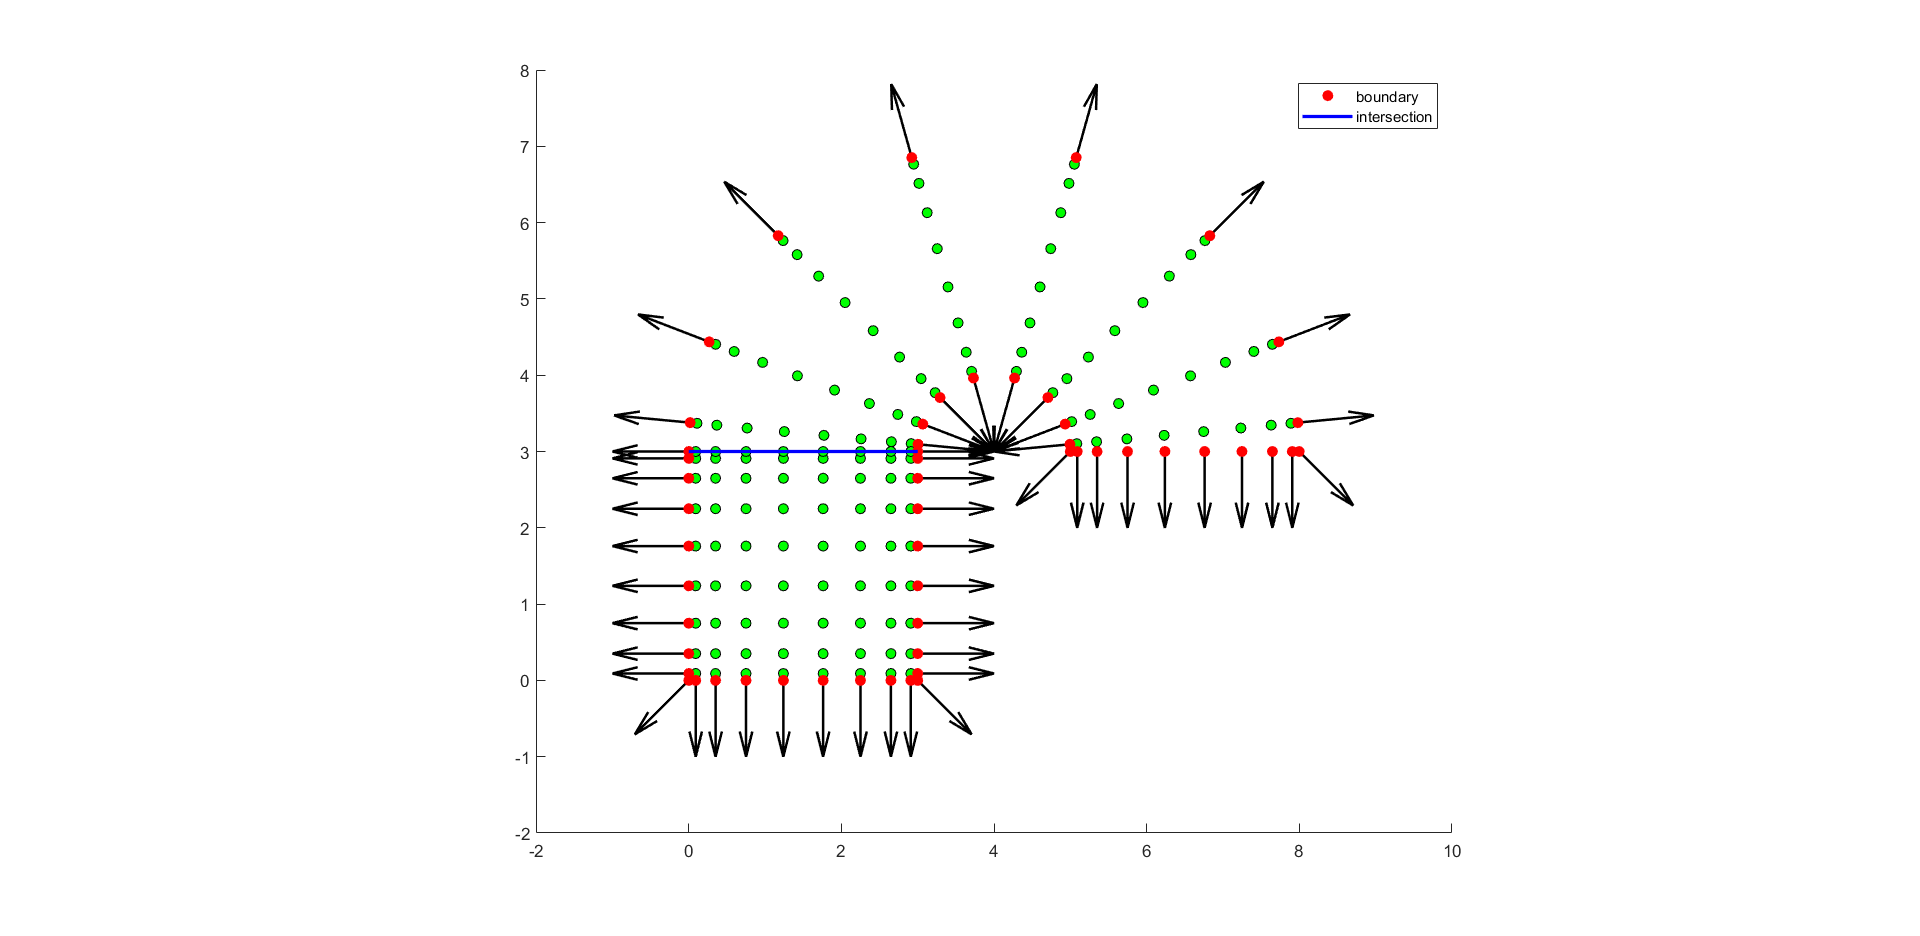
\includegraphics[scale=0.5]{normals.png}
		\caption{Needs fixing} 
		\label{F1}
	\end{figure}
\\
\\
The final aspect to be considered is the convolution matrix, which is needed to compute convolution integrals. It is computed in a similarly straightforward way, but since convolution is a global operation, it is not as simple as stacking the convolution matrices for the individual shapes, as is done for differentiation, integration and interpolation. 
The convolution integral is defined as:
\begin{align*}
	\left(n \star \chi \right) (y) = \int \chi (y - \tilde y) n (\tilde y) d \tilde y.
\end{align*}
As explained in \cite{GoddardPseudospectralCode1} in detail, $\chi$ at $y - \tilde y$ is evaluated for all points in the multishape domain and transformed into a matrix $\text{diag} \left(\chi\right)$. This is integrated, using the stacked integration vector, to result in the convolution matrix, which can then be applied to a density $n$.


\section{Validation Tests}
Several examples are run, using exact solutions, to test whether the multishape code works. This is done using an exact solution to the advection diffusion equation on an infinite domain, so that Dirichlet boundary conditions, matching the value of the exact solution on the boundary of the multishape, can be applied.
The exact solution is:
\begin{align*}
	\rho &= \exp(\alpha t + \beta_1 y_1 + \beta_2 y_2)\\
	\mathbf v &= \left(\beta_1 - \frac{\alpha}{2 \beta_1} + p_1\exp(-\beta_1 y_1) , \beta_2 - \frac{\alpha}{2 \beta_2} + p_2\exp(-\beta_2 y_2) \right),
\end{align*}
where $\beta_1 = -1$, $\beta_2 = 1$, $\alpha = 0.5$, $p_1 = -1$ and $p_2 = 1$.
At first, we compare the exact solution on a box of dimensions $[0,2] \times [0,2] $ with a multishape consisting of two boxes of dimensions $[0,2] \times [0,1]$ and $[0,2] \times [1,2]$, see Figure \ref{F2}. The question is whether the results of the PDE on the box and the dissected box are equal. Each of the shapes are discretized with $N = 20$ points in each spatial direction, which means that the dissected box has more points in total than the original box.
The relative error between the solutions on the two boxes is $1.0034 \times 10^{-10}$. 
When reducing the number of points in the dissected box to $N = 10$ per shape, while keeping $N = 20$ in the single shape box, the relative error in solution is $2.565 \times 10^{-10}$. The solution can be seen in Figure \ref{F3}.

	\begin{figure}[h]
		\centering
		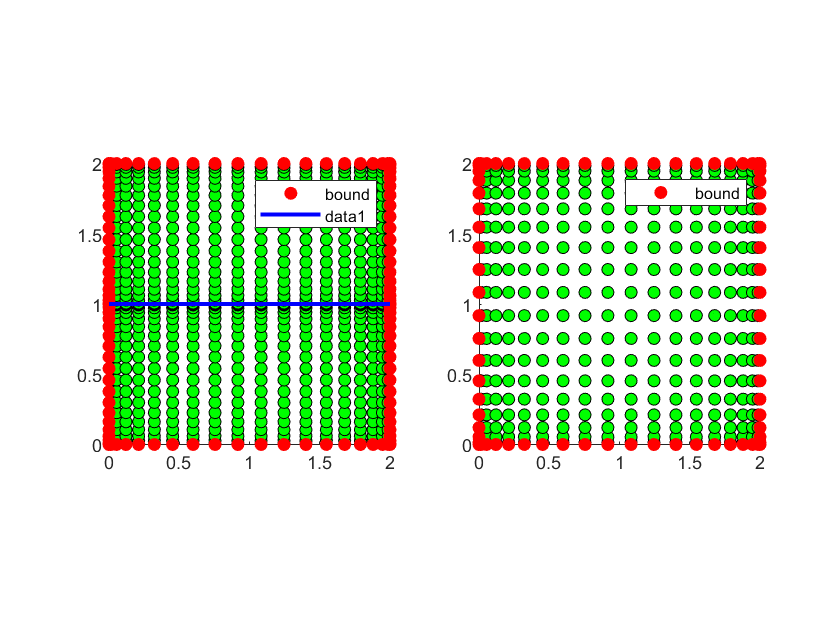
\includegraphics[scale=0.5]{disect1.png}
		\caption{The box and dissected box with $N = 20$} 
		\label{F2}
	\end{figure}

	\begin{figure}[h]
		\centering
		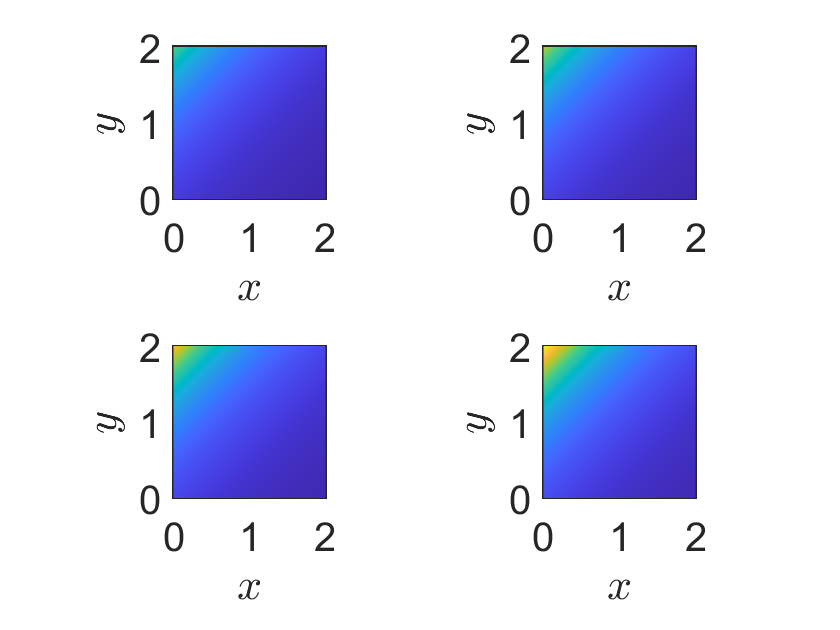
\includegraphics[scale=0.5]{disect2.png}
		\caption{Exact solution on the box} 
		\label{F3}
	\end{figure}
The same test can be done for a wedge. Here, a single wedge and a dissected version are considered, see Figure \ref{F4}. The error in solution between the two approaches with $N = 20$ is $2.0195 \times 10^{-7}$ and with $N = 10$ for each of the two shapes in the disected wedge and $N = 20$ in the full wedge the error is $3.349 \times 10^{-6}$. For $N = 30$ for the shapes in both domains the error is $9.8444 \times 10^{-11}$. This shows that the solution on the wedge is harder to compute accurately and needs more points as compared to the box. The solution can be seen in Figure \ref{F5}.
	\begin{figure}[h]
	\centering
	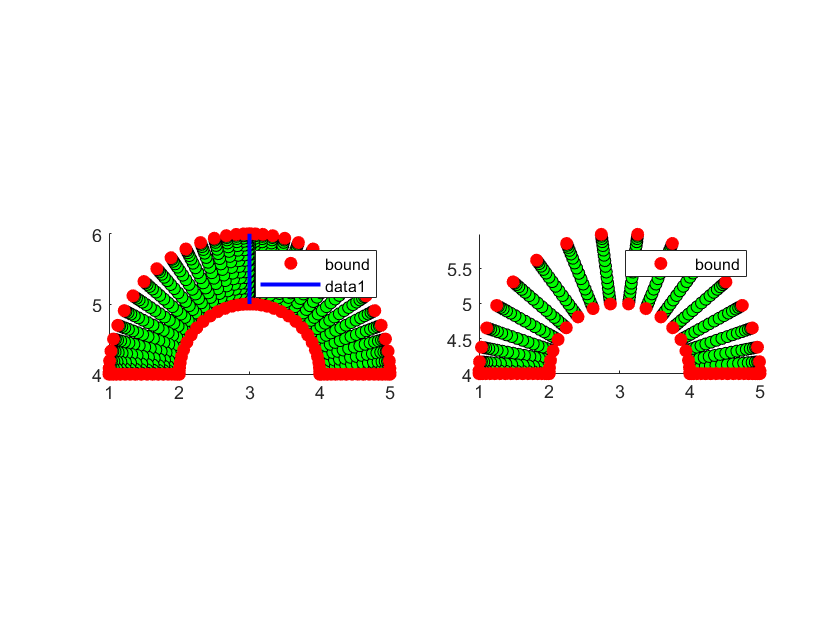
\includegraphics[scale=0.5]{disectW1.png}
	\caption{The wedge and dissected wedge with $N = 20$} 
	\label{F4}
\end{figure}

\begin{figure}[h]
	\centering
	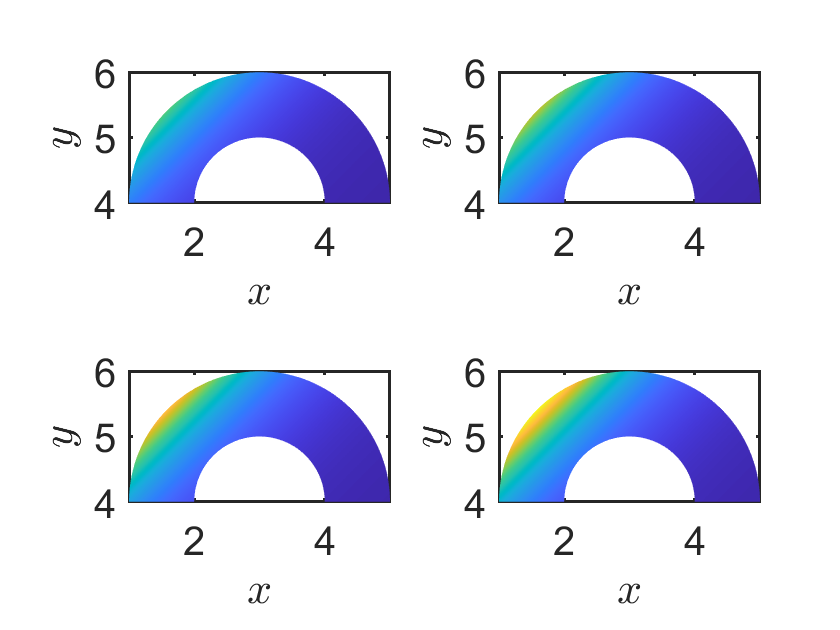
\includegraphics[scale=0.5]{disectW2.png}
	\caption{Exact solution on the wedge} 
	\label{F5}
\end{figure}

Next the advection diffusion equation is solved on a multishape which is composed of four quadrilaterals, see Figure \ref{F6}. The relative error for $N = 20$ on each shape as compared to the exact solution is $2.3321 \times 10^{-9}$. 
\begin{figure}[h]
	\centering
	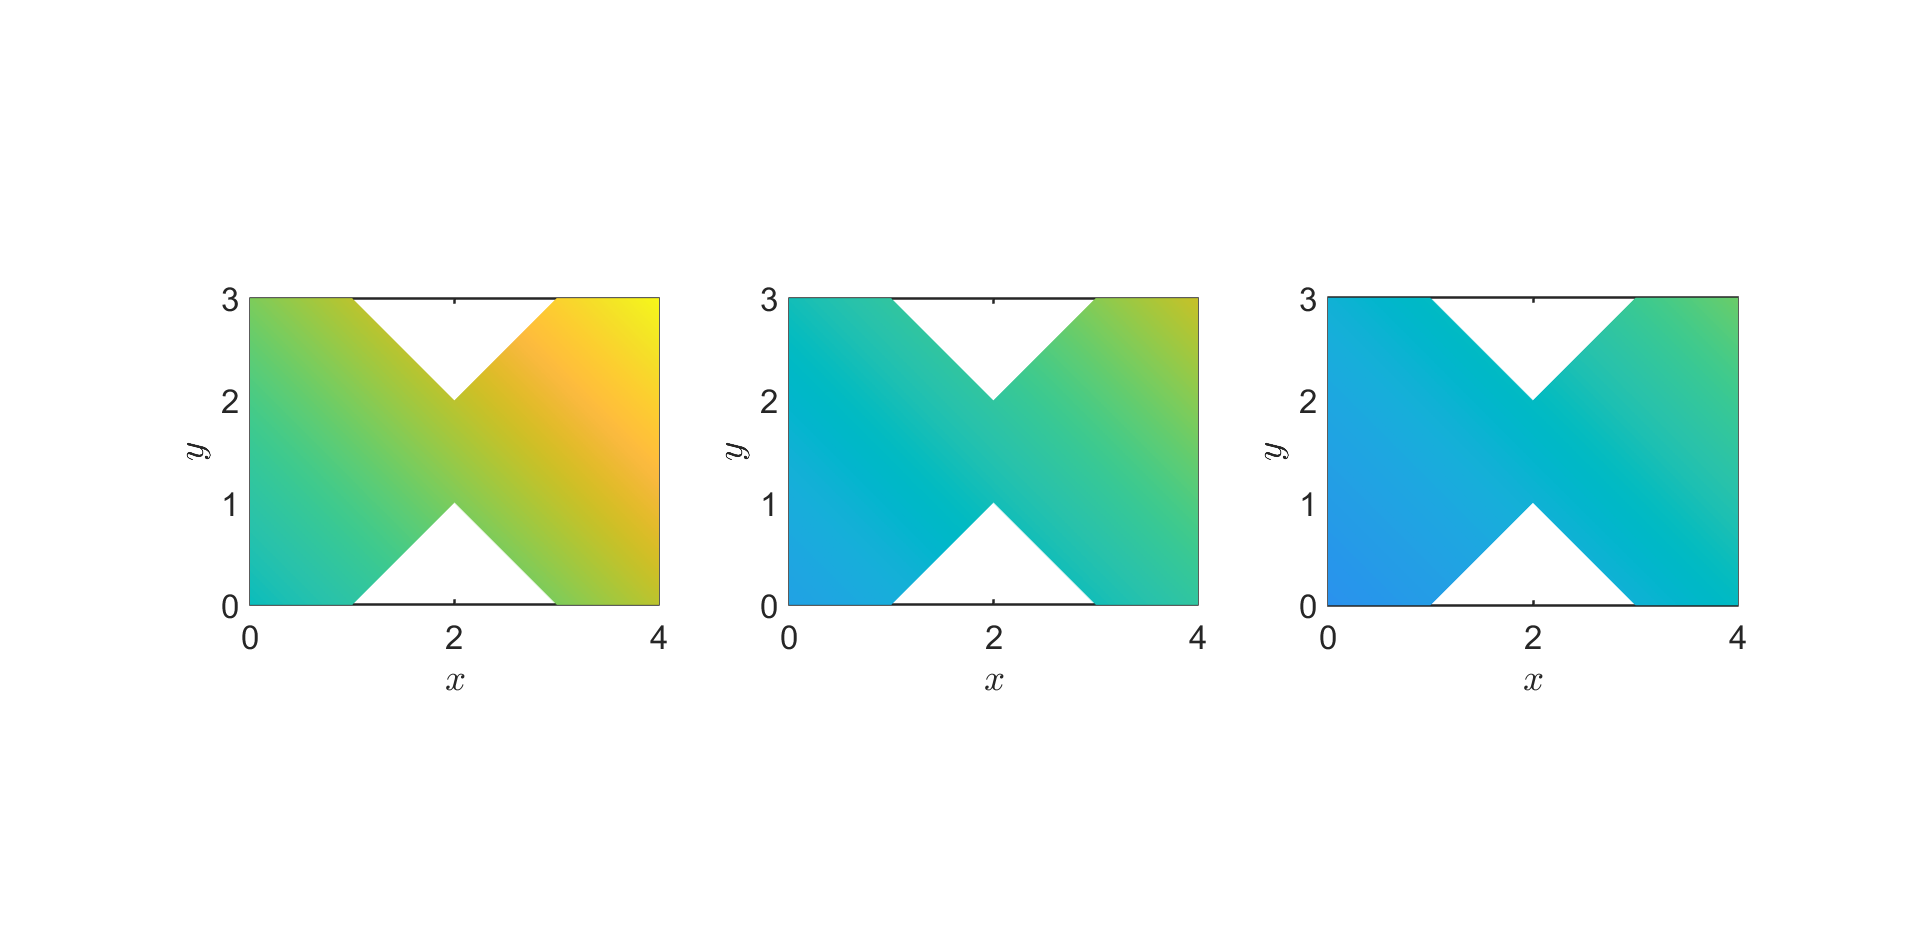
\includegraphics[scale=0.5]{example1.png}
	\caption{Example 1 multishape} 
	\label{F6}
\end{figure}
The same is done for a second example involving a wedge, see Figure \ref{F7}. The relative error to the exact solution is $1.3128 \times 10^{-7}$, when choosing $N= 20$ per shape. We again observe that a larger error is introduced when the multishape includes a wedge as compared to Example 1, which only included quadrilaterals. For $N = 30$ the error decreases to $2.2463 \times 10^{-9}$.

\begin{figure}[h]
	\centering
	\includegraphics[scale=0.5]{example2.png}
	\caption{Example 2 multishape} 
	\label{F7}
\end{figure}


\section{Forward Problems on multishapes}

The first example is solving an advection diffusion problem on a multishape consisting of two quadrilaterals and two wedges, with constant velocity of strength ten. The initial condition for this problem is:
 \begin{align*}
 	\rho_0 = \exp( -2(y_1 -0.5)^2 - 2 (y_2 + 1)^2).
 \end{align*}
The result, evaluated for $N= 20$ on each shape, can be seen in Figure \ref{F8}.

\begin{figure}[h]
	\centering
	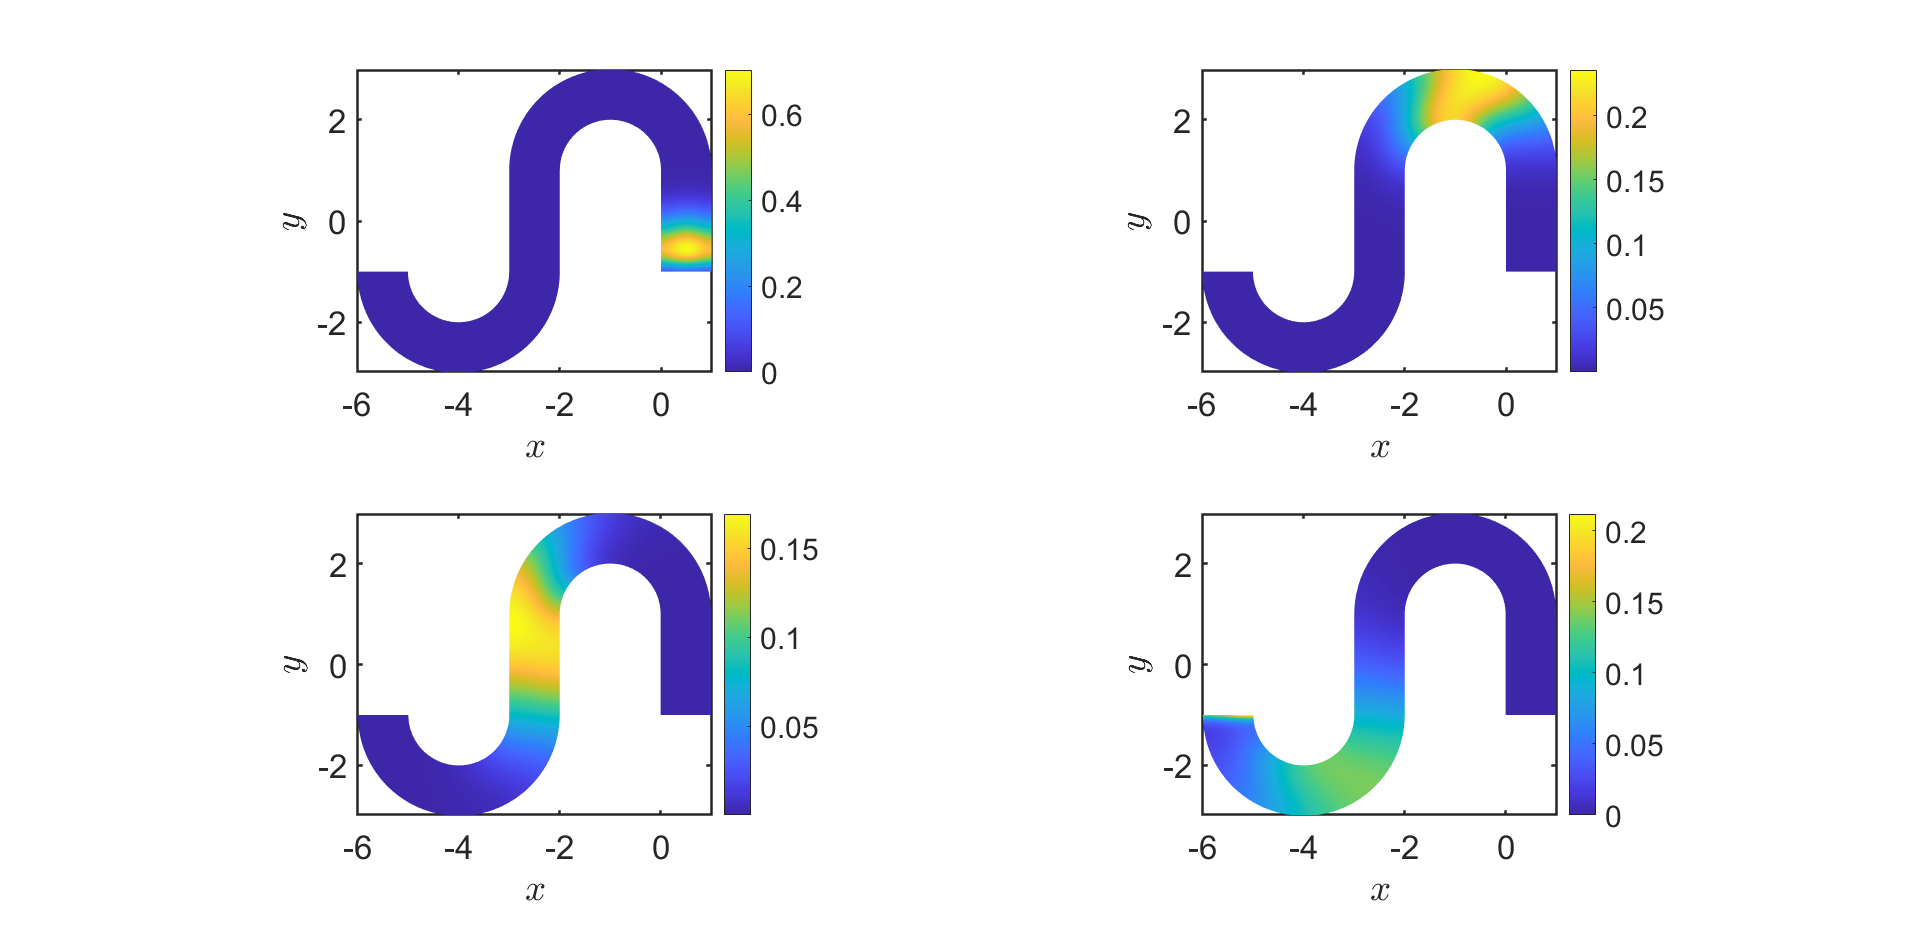
\includegraphics[scale=0.5]{ex1.png}
	\caption{Forward Problem 1}
	\label{F8}
\end{figure}

In a second example, the velocity is of strength $5$ and the initial condition is:
 \begin{align*}
	\rho_0 = \exp( -2(y_1 -0.5)^2 - 2 (y_2 - 1.5)^2).
\end{align*}
The result, which is computed on a multishape made up of four quadrilaterals into a channel, can be seen in Figure \ref{F9}.

\begin{figure}[h]
	\centering
	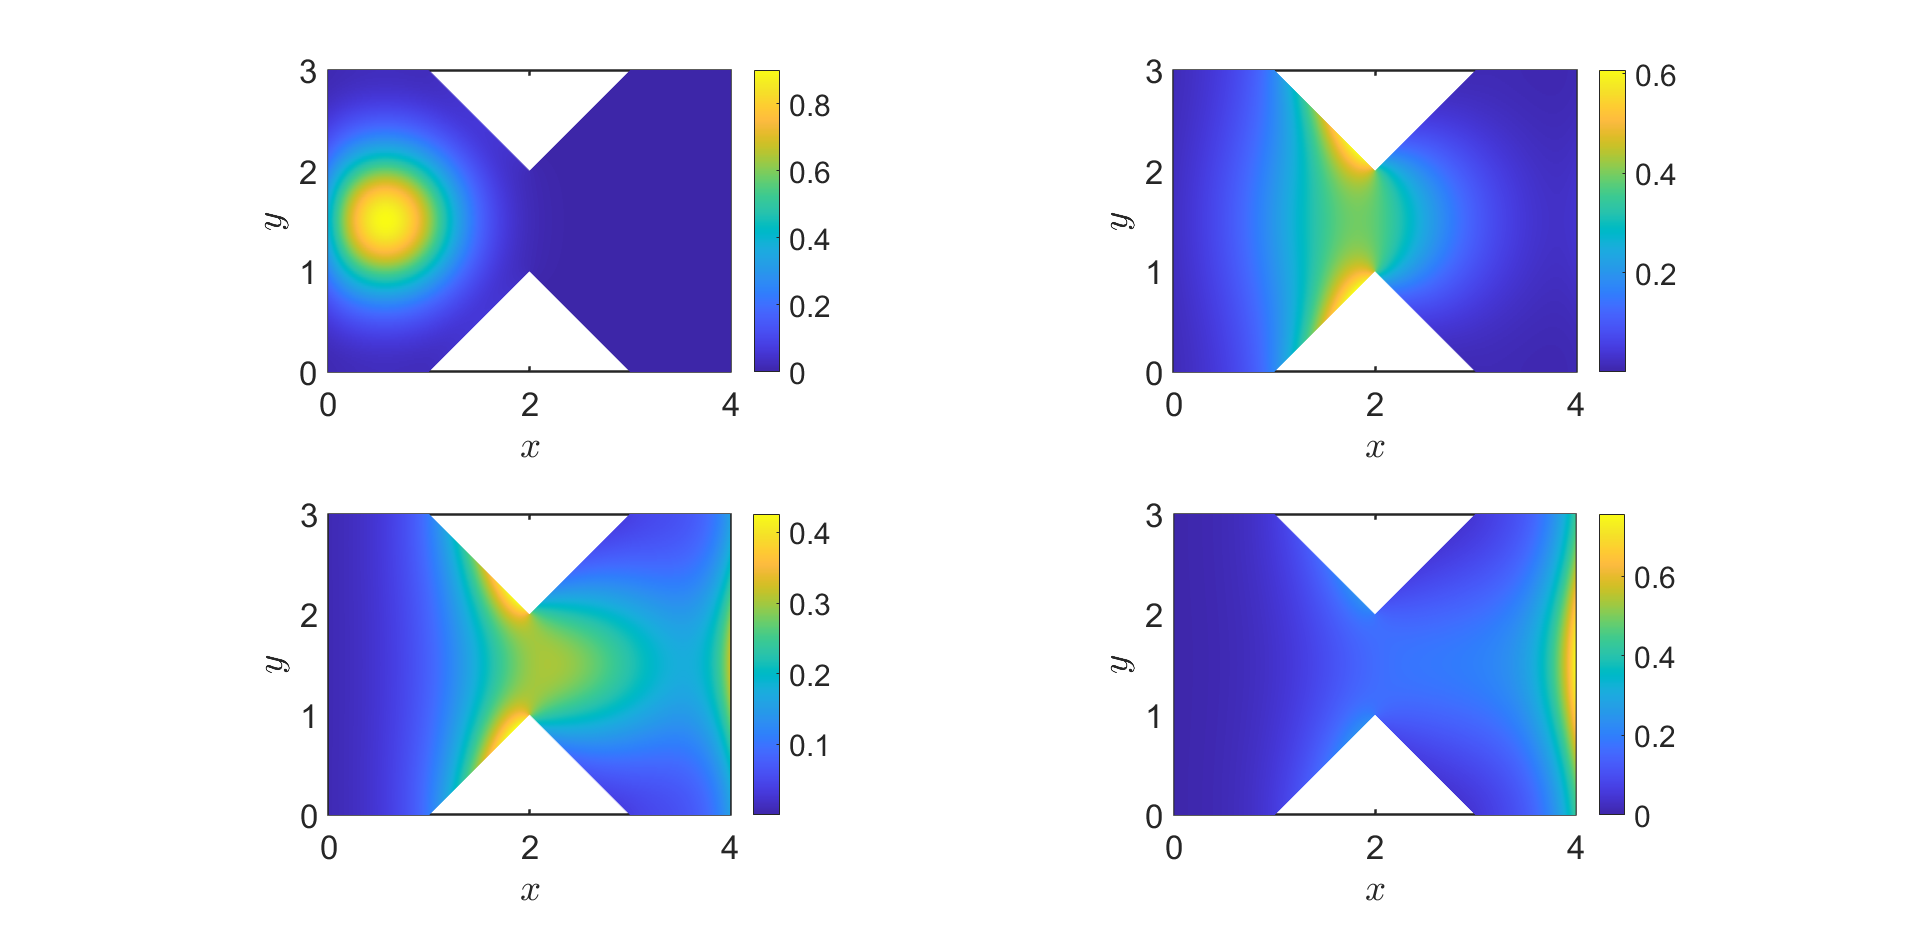
\includegraphics[scale=0.5]{ex2.png}
	\caption{Forward Problem 2}
	\label{F9}
\end{figure}








\pagebreak	
\bibliography{GeneralBib}
\bibliographystyle{unsrt}
\end{document}	
	
	
	\section{Derivation of Optimality Conditions with Periodic Boundary Conditions}
	+++++ Change notation for j ++++++
	We consider the advection diffusion equation with periodic boundary conditions and a corresponding OCP:
	\begin{align*}
		&\min \frac{1}{2}|| \rho - \hr||^2 + \frac{\beta}{2}||\w||^2\\
		&\text{subject to:}\\
		&\frac{\partial \rho}{\partial t} = \nabla \cdot \left(\nabla \rho - \rho \w\right) = -\nabla \cdot \jf\\
		& \rho|_{\partial \Omega_l} = \rho|_{\partial \Omega_r}\\
		& \rho|_{\partial \Omega_t} = \rho|_{\partial \Omega_b}\\
		& - \jf \cdot \n |_{\partial \Omega_l}= - \jf \cdot \n|_{\partial \Omega_r}
	\end{align*}
	such that $\partial\Omega_l \cup \partial\Omega_r = \partial \Omega$ and the abbreviations corresponding to left and right respectively. Top and bottom boundaries are omitted, since, as shown in the previous section, they follow analogously and are independent of the results on the left and right boundary. Note that we could match first derivatives instead of the flux on the boundary.
	The relevant part of the Lagrangian is then:
	\begin{align*}
		\mathcal{L} &= ... -\int_0^T \int_\Omega \left(\frac{\partial \rho}{\partial t} + \nabla \cdot \jf\right)q dr dt - \int_0^T \int_{\partial \Omega_l} \left(- \rho q_1 - \jf \cdot \n q_2 \right) dr  + \int_{\partial \Omega_r} \left(\rho q_1 +  \jf \cdot \n q_2  \right)  dr .
	\end{align*}
	Integrating by parts, and omitting terms in $\Omega$, gives:
	\begin{align*}
		\mathcal{L} &= ... - \int_0^T \int_{\partial \Omega} q \jf  \cdot \n + \mathbf{k}(\rho, q) \cdot \n  dr dt - \int_0^T \int_{\partial \Omega_l} \left(- \rho q_1 - \jf \cdot \n q_2 \right)   dr  + \int_{\partial \Omega_r} \left(\rho q_1 + \jf \cdot \n q_2 \right)   dr, 
	\end{align*}
	where $\mathbf{k}$ are any terms arising from integrating by parts a second time.
	We now need to take the Frech\'et derivative of $\jf$ with respect to $\rho$. This cannot be done in general, because $\jf$ does not only depend on $\rho$ but also on $\mathbf r$. In each case we need to calculate:
	\begin{align*}
		\jf'(h) := \jf (\rho + h) - \jf (\rho).
	\end{align*}
	Similarly, we need to take the derivative of $\mathbf k$ and denote it by $\mathbf{k}'$.
	Denoting this Frech\'et derivative by $\jf'(h)$ we can write out further terms as follows:
	\begin{align*}
		\mathcal{L}_\rho &= ... - \int_0^T \int_{\partial \Omega} q \jf'(h)   \cdot \n + \mathbf{k}' \cdot \n dr dt - \int_0^T \int_{\partial \Omega_l} \left(- h q_1 - \jf'(h)  \cdot \n q_2 \right)   dr  + \int_{\partial \Omega_r} \left(h q_1 + \jf'(h)  \cdot \n q_2 \right)   dr dt. 
	\end{align*}
	When writing out the terms explicitly we pay attention to the fact that $\n|_{\partial \Omega_l} = - \n|_{\partial \Omega_r}$ and $\n|_{\partial \Omega_t} = - \n|_{\partial \Omega_b}$.
	\begin{align*}
		\mathcal{L}_\rho &= ... - \int_0^T \int_{\partial \Omega_l} \left(- h q_1 + q \jf'(h)   \cdot \n  + \mathbf{k}' \cdot \n- \jf'(h)  \cdot \n q_2 \right)   dr  \\
		&+ \int_{\partial \Omega_r} \left(h q_1 - q \jf'(h)   \cdot \n - \mathbf{k}' \cdot \n+ \jf'(h)  \cdot \n q_2 \right)   dr dt .
	\end{align*}
	In order to proceed further, we need to split up $\jf'(h)$ into two parts as follows:
	\begin{align*}
		\jf'(h) = \jf'_1(h) + h \jf'_2,
	\end{align*}
	so that $\jf'_1$ is applied to $h$, since it depends on $\mathbf{r}$ as well (e.g. the Frech\'et derivative of $\nabla \rho$) and $\jf'_2$ is applied to another function and multiplied by $h$ (e.g. h $\frac{\partial }{\partial n}$ applied to $q$). We do the same for $\mathbf k'$.
	We then have:
	\begin{align*}
		\mathcal{L}_\rho &= ... - \int_0^T \int_{\partial \Omega_l} \left(- h q_1 + q \jf_1'(h)   \cdot \n + \mathbf{k}_1' \cdot \n - \jf_1'(h)  \cdot \n q_2  + h \jf'_2 q \cdot \n + h \mathbf{k}_2' \cdot \n-  h \jf'_2 q_2 \cdot \n \right)   dr  \\
		&+ \int_{\partial \Omega_r} \left( h q_1 - q \jf_1'(h)   \cdot \n -\mathbf{k}_1' \cdot \n+ \jf_1'(h)  \cdot \n q_2 - h\mathbf{k}_2' \cdot \n - h \jf'_2 q \cdot \n +  h \jf'_2 q_2 \cdot \n \right)   dr dt.
	\end{align*}
	Considering $\jf'_1 \neq 0$, we get:
	\begin{align*}
		\int_0^T \int_{\partial \Omega_l} \left( q \jf_1'(h)   \cdot \n  + \mathbf{k}_1' \cdot \n - \jf_1'(h)  \cdot \n q_2  \right)   dr  + \int_{\partial \Omega_r} \left(-q \jf_1'(h)   \cdot \n - \mathbf{k}_1' \cdot \n + \jf_1'(h)  \cdot \n q_2  \right)   dr dt = 0 .
	\end{align*}
	Note that if $\mathbf{k}_1' = 0$, we can conclude that $q = q_2$ on both boundaries.
	In general, $q_2|_{\partial \Omega_l} = q_2|_{\partial \Omega_r}$, i.e. $q_2$ is constant on the boundary, and an equivalent statement holds for $q_1$. Therefore, we have that:
	\begin{align*}
		\int_0^T \int_{\partial \Omega_l}  q \jf_1'(h)   \cdot \n  +\mathbf{k}_1' \cdot \n   dr dt = \int_0^T \int_{\partial \Omega_r} q \jf_1'(h)   \cdot \n  +  \mathbf{k}_1' \cdot \n  dr dt .
	\end{align*}
	Writing this in terms of the integrand only can be done for each specific case of $\jf_1'$ and $\mathbf{k}_1'$. 
	 Now considering all terms such that $h \neq 0$ on each boundary separately, we get:
	 \begin{align*}
	 	&\int_0^T \int_{\partial \Omega_l} \left(- h q_1  + h \jf'_2 q \cdot \n + h\mathbf{k}_2' \cdot \n-  h \jf'_2 q_2 \cdot \n \right)   dr  dt =0 \\
	 	&\int_0^T \int_{\partial \Omega_r} \left( h q_1  - h \jf'_2 q \cdot \n - h\mathbf{k}_2' \cdot \n + h \jf'_2 q_2 \cdot \n \right)   dr  dt =0 ,
	 \end{align*}
 	and so, as in the previous sections, we have:
 	\begin{align*}
 		q_1 &=   \jf'_2 q \cdot \n + \mathbf{k}_2' \cdot \n - \jf'_2 q_2 \cdot \n |_{\partial \Omega_l} \\
		q_1 &=  \jf'_2 q \cdot \n + \mathbf{k}_2' \cdot \n -\jf'_2 q_2 \cdot \n |_{\partial \Omega_r}, 
 	\end{align*}
	which gives:
	\begin{align*}
		  \jf'_2 q \cdot \n +  \mathbf{k}_2' \cdot \n - \jf'_2 q_2 \cdot \n |_{\partial \Omega_l} =  \jf'_2 q \cdot \n + \mathbf{k}_2' \cdot \n - \jf'_2 q_2 \cdot \n |_{\partial \Omega_r}.
	\end{align*}
	If $\mathbf{k}_1' = 0$ and so $q = q_2$ as discussed above, the two terms involving $\jf_2'$ cancel and we get
	\begin{align*}
	 \mathbf{k}_2' \cdot \n  |_{\partial \Omega_l} =   \mathbf{k}_2' \cdot \n  |_{\partial \Omega_r}.
	\end{align*}
	Otherwise, since $q_2|_{\partial \Omega_l} = q_2|_{\partial \Omega_r}$, we can at least conclude that:
	\begin{align*}
		\jf'_2 q \cdot \n + \mathbf{k}_2' \cdot \n  |_{\partial \Omega_l} =  \jf'_2 q \cdot \n + \mathbf{k}_2' \cdot \n  |_{\partial \Omega_r}.
	\end{align*}
	\\
	\\
	An example: Let $\jf = \nabla \rho - \rho \w$ as above. Then we have that $\jf_1'(h) = \nabla h$ and $\jf_2' = \w $. From integration by parts we will get that $\mathbf k = - \rho \nabla q$, so $\mathbf k_1' = 0$ and $\mathbf k_2' = -  \nabla q$.
	We therefore get that:
	\begin{align*}
		& \nabla q \cdot \n |_{\partial \Omega_l} = \nabla q \cdot \n |_{\partial \Omega_r},
	\end{align*}
	and
	\begin{align*}
		\int_0^T \int_{\partial \Omega_l}  q \nabla h   \cdot \n    dr dt = \int_0^T \int_{\partial \Omega_r} q \nabla h  \cdot \n    dr dt,
	\end{align*}
	and so 
	\begin{align*}
		q |_{\partial \Omega_l} = q|_{\partial \Omega_r},
	\end{align*}
	as required.
	\section{Sedimentation}
	\subsection{Forward Problem}
	We are interested in modelling sedimentation processes. In order to achieve this, the advection-diffusion equation with mean-field interaction term has to be modified to include an approximation to volume exclusion. Archer and Malijevs\'y \cite{ArcherSed1} have achieved this using the following model to describe sedimentation processes. 
The modelling equations are:
\begin{align*}
	&\frac{\partial \rho}{\partial t^*} = \Gamma\nabla \cdot \left(  \rho \nabla \frac{\delta F[\rho]}{\delta \rho} \right) ,
\end{align*}
where $\Gamma$ is the diffusion coefficient. 	
We can rescale this equation as done in \cite{ArcherSed1} using the relationship $t = t^*/ \tau_B$, where $\tau_B = \beta \sigma^2 / \Gamma$ is the Brownian time scale.
Applying this rescaling we get:
\begin{align}\label{Eq1}
	&\frac{\partial \rho}{\partial t} = \beta \sigma^2\nabla \cdot \left(  \rho \nabla \frac{\delta F[\rho]}{\delta \rho} \right).
\end{align}
The free energy functional considered in \cite{ArcherSed1} is:
\begin{align*}
	F[\rho] &= \frac{1}{\beta} \int \rho (\ln \Lambda^2 \rho - 1) + f_{HDA} dr + \frac{1}{2}\int \int \rho(r) \rho(r') V_2(|r - r'|) dr dr' + \int \rho V_{ext} dr,
\end{align*}
where $f_{HDA}$ the approximate free energy density describing the volume exclusion through hard disks. The external potential is defined as:
\begin{align*}
	V_{ext} &= c y, \quad \text{for } \quad 0 < y < L,
\end{align*}
where $c$ a constant and $L$ is the height of a rectangular domain. Outside these bounds $V_{ext} = \infty$. 
Furthermore, we have the pair potential:
\begin{align*}
	V_2 = exp(-r/\sigma),
\end{align*}
where $\sigma$ is the particle diameter of the hard sphere particle.


\subsubsection{The Hard Disk Approximation}
The part of the free energy functional, which accounts for the hard disk approximation, is:
\begin{align*}
	F_{HDA}[\rho] &= \frac{1}{\beta} \int  f_{HDA} dr = \frac{1}{\beta} \int   -  \rho - \rho \ln(1 - \eta) + \frac{\rho}{1 - \eta} dr,
\end{align*}
where $\eta = a \rho = \frac{\pi \sigma^2}{4} \rho$.
This can be thought of as the bulk fluid, one species, two dimensional approximation of Fundamental Measure Theory (FMT)  \cite{RosenfeldFMT}, which is a Density Functional Theory for hard sphere mixtures. The basis of this theory is that the excess free energy functional is of the form:
\begin{align*}
	\beta F_{ex}[{\rho_i}] = \int \Phi({n_\alpha(r')})d^3r',
\end{align*} 
where $i$ is the species count and $\Phi$ is a function of the weighted densities $n_\alpha$. By now there are many different versions of $\Phi$, yielding approximations of $F_{ex}$ with different limitations, see \cite{Roth_2010FMTReview}. Rosenfeld's original version is defined as:
	\begin{align*}
	\Phi = -n_0 \ln(1-n_3) + \frac{n_1 n_2 - \mathbf{n_1} \cdot \mathbf{n_2}}{1-n_3} + \frac{n_2^3 - 3n_2 \mathbf{n_2} \cdot \mathbf{n_2}}{24 \pi (1-n_3)^2}.
	\end{align*}
The weighted densities for $\nu$ species are:
	\begin{align} \label{eqn:WeightedDensities}
		n_\alpha (r) = \sum_{i=1}^\nu \int \rho_i(r') \omega_\alpha^i(r -r').
	\end{align}
The weight functions chosen by Rosenfeld are:
\begin{align*}
	&\omega_3^i = \Theta(R_i -r),\quad \omega_2^i = \delta(R_i -r),\quad \mathbf{\omega_2^i} = \frac{\mathbf r}{r}\delta (R_i -r),\quad \\
	&\omega_1^i = \omega_2^i/(4 \pi R_i), \quad \omega_0^i = \omega_2^i/(4\pi R_i^2), \quad \mathbf{\omega_1^i} = \mathbf{\omega_2^i}/(4 \pi R_i),
\end{align*}
where $R_i$ is the radius of the excluded volume, $\Theta$ is the Heaviside function and $\delta$ is the delta function. Integrating over $\omega_\alpha$, with $\alpha = 0,1,2,3$, we get the fundamental measures of a sphere: volume, surface area, radius and the Euler characteristic \cite{Roth_2010FMTReview} \cite{RosenfeldFMT}.
\\
Based on this theory for three dimensional spheres and the fact that the theory for hard rods is known exactly \cite{Percus1976}, Rosenfeld derived a version of this approach for two dimensional hard disks \cite{Rosenfeld2DInterp}. However, some additional approximations have to be made when choosing the weighted densities, which is not necessary in one and three dimensions. The resulting equation is:
\begin{align*}
	\Phi = - n_0 \ln(1-n_3) + \frac{1}{4 \pi} \frac{n_2 n_2}{1-n_3} + \frac{1}{4 \pi} \frac{\mathbf{n_2} \cdot \mathbf{n_2}}{1-n_3}.
\end{align*}
\\
In the uniform limit, for one particle species, we get that:
\begin{align*}
	n_0 = \rho, \quad n_2 = 2 \pi R \rho, \quad n_3 = \pi R^2 \rho,
\end{align*}
by solving the integrals in \eqref{eqn:WeightedDensities}, using spherical polar coordinates, with $\rho = \rho_{\text{bulk}}$, a constant. 
Substituting this in the 2D version of $\Phi$ gives:
\begin{align*}
	\Phi = - \rho \ln (1- \pi R^2 \rho) + \frac{1}{4 \pi} \frac{4\pi^2 R^2 \rho^2}{1 - \pi R^2 \rho} + \frac{1}{4 \pi}\frac{\mathbf{n_2} \cdot \mathbf{n_2}}{1 - \pi R^2 \rho},
\end{align*}
where $\mathbf{n_2} = \mathbf 0$ in the uniform limit, since the corresponding equation in \eqref{eqn:WeightedDensities} is an integral over an odd function.
Noting that $R = \sigma/2$ and $\eta = \pi \sigma^2 \rho /4$, we get that:
\begin{align} \label{eqn:SPTFunctional2D}
	\Phi = - \rho \ln (1- \eta) + \frac{\rho \eta}{1 - \eta} = \rho \left(-\ln(1-\eta) + \frac{1}{1- \eta} -1 \right).
\end{align} 
This expression for the free energy for the bulk fluid is the same as derived by scaled particle theory (SPT) \cite{Reiss1959}, \cite{Reiss1960}, \cite{Helfand1961}, which also coincides with the Percus-Yevic compressibility equation \cite{PercusYevick1}, as detailed in \cite{RosenfeldSPT}.
While the SPT approximation \eqref{eqn:SPTFunctional2D} and its three-dimensional equivalent are used in classical DFT, see \cite{DFTWinkelmann2001}, \cite{DFTRoth1}, \cite{DFTRoth2}, \cite{DFTGonzalez1997}, \cite{DFTCuesta2008}, \cite{DFTLoewen2002}, and other statistical mechanics approaches, see \cite{GrafLoewen1999}, \cite{DuBois2002}, \cite{Chamoux1998}, \cite{Chamoux1996}, in dynamical DFT it is not commonly applied and only the work of Archer et al. \cite{ArcherSed1}, \cite{ArcherSed2008}, \cite{ArcherSed2011}, \cite{ArcherSed2013}, is known to us in this context.

\subsubsection{Deriving the equation of motion}
Since we are interested in the equation of motion, we need to calculate $ \nabla \cdot \left(\rho \nabla \frac{\delta F_{HDA}[\rho]}{\delta \rho} \right)$. We combine $F_{HDA}$ and $F_{ID} = \int_\Omega \rho (\ln \Lambda^2 \rho - 1) dr$ here so that we have:
\begin{align*}
	F_{N} = F_{HDA} + F_{ID}.
\end{align*}
Taking the functional derivative of $F_{N}$ gives:
\begin{align*}
	\frac{\delta F_{N}[\rho]}{\delta \rho} &= \frac{1}{\beta} \bigg(1 + \ln \rho + \Lambda^2 -2 - \ln(1-\eta) + a \frac{\rho}{1 - \eta} + \frac{1}{1 - \eta} + a \frac{\rho}{(1 - \eta)^2}  \bigg)\\
	&= \frac{1}{\beta} \bigg(1 + \ln \rho + \Lambda^2 -2 - \ln(1-\eta) + \frac{1}{(\eta - 1)^2} - \frac{1}{\eta - 1}  - 1\bigg)\\
	&= \frac{1}{\beta} \bigg( \ln \rho + \Lambda^2 - 2 - \ln(1-\eta) - \frac{\eta - 2}{(\eta - 1)^2}  \bigg),
\end{align*}
using partial fractions. Then:
\begin{align*}
	\nabla \frac{\delta F_{N}[\rho]}{\delta \rho} &= \frac{1}{\beta} \bigg( \nabla\ln \rho + \nabla(\Lambda^2 - 2) - \nabla\ln(1-\eta) - \nabla\frac{\eta - 2}{(\eta - 1)^2}  \bigg)\\
	& = \frac{1}{\beta} \bigg( \frac{\nabla \rho}{\rho} - \frac{\nabla( 1- \eta)}{1 - \eta} - \nabla\frac{\eta - 2}{(\eta - 1)^2}  \bigg)\\
	& = \frac{1}{\beta} \bigg( \frac{\nabla \rho}{\rho} + \frac{\nabla \eta}{1 - \eta} - \nabla\frac{\eta - 2}{(\eta - 1)^2}  \bigg).
\end{align*}
Then multiplying by $\rho$ gives:
\begin{align*}
	\rho \nabla \frac{\delta F_{N}[\rho]}{\delta \rho} &= \frac{1}{\beta} \bigg( \nabla \rho +   \frac{\rho \nabla \eta}{1 - \eta} - \rho \nabla\frac{\eta - 2}{(\eta - 1)^2}  \bigg)\\
	&= \frac{1}{\beta} \bigg( \nabla \rho +   \frac{\eta\nabla \rho}{1 - \eta} - \rho \nabla\frac{\eta - 2}{(\eta - 1)^2}  \bigg)\\
	&= \frac{1}{\beta} \bigg( \nabla \rho + \frac{\nabla \rho}{1 - \eta} - \nabla \rho - \rho \nabla\frac{\eta - 2}{(\eta - 1)^2}  \bigg)\\
	&= \frac{1}{\beta} \bigg(  \frac{\nabla \rho}{1 - \eta}  - \rho \nabla\frac{\eta - 2}{(\eta - 1)^2}  \bigg).
\end{align*}
Finally we take the divergence:
\begin{align*}
	\nabla \cdot \bigg(\rho \nabla \frac{\delta F_{N}[\rho]}{\delta \rho}\bigg) &= \frac{1}{\beta} \bigg( \nabla  \cdot \left(  \frac{\nabla \rho}{1 - \eta} \right) - \nabla  \cdot \left(\rho \nabla\frac{\eta - 2}{(\eta - 1)^2} \right) \bigg)\\
	&= \frac{1}{\beta} \bigg( \frac{\nabla^2 \rho}{1 - \eta} +  \nabla \rho \cdot \nabla \frac{1}{1 - \eta} - \nabla \rho \cdot \nabla \frac{\eta - 2}{(\eta - 1)^2} - \rho \nabla^2\frac{\eta - 2}{(\eta - 1)^2} \bigg)\\
	&= \frac{1}{\beta} \bigg( \frac{\nabla^2 \rho}{1 - \eta} +  \nabla \rho \cdot \nabla \frac{(3- 2 \eta)}{(1 - \eta)^2}  - \rho \nabla^2\frac{\eta - 2}{(\eta - 1)^2} \bigg).
\end{align*}
	\subsection{Derivation of Optimality Conditions}
	One optimal control problem to consider is:
\begin{align}\label{eq:OCP1}
	&J = \frac{1}{2}\int_0^T \int_\Omega (\rho - \widehat \rho)^2 dr dt + \frac{\beta}{2} \int_0^T\int_\Omega \w(r)^2 dr \notag\\
	&\text{subject to:}\\
	&\frac{\partial \rho}{\partial t} = \beta \sigma^2 \bigg( \nabla \cdot (\rho \nabla V_{ext}) - \nabla (\rho \w) + \nabla \cdot \left(\rho \nabla \frac{\delta F_{N}[\rho]}{\delta \rho}\right) + \kappa \int_\Omega \rho(r) \rho(r') \K(r,r')dr\bigg), \notag
\end{align}
where $\K(r,r') = \nabla V_2$.
We consider the terms of the PDE and the boundary conditions separately here.
\subsubsection{Calculating Frech\'et Derivatives}
In order to derive the optimalty conditions for the above OCP, we need to calculate the Frech\'et derivatives of the following terms:
\begin{align*}
	\nabla \cdot \bigg(\rho \nabla \frac{\delta F_{N}[\rho]}{\delta \rho}\bigg)
	&= \frac{1}{\beta} \bigg( \frac{\nabla^2 \rho}{1 - \eta} +  \nabla \rho \cdot \nabla \frac{(3- 2 \eta)}{(1 - \eta)^2}  - \rho \nabla^2\frac{\eta - 2}{(\eta - 1)^2} \bigg),
\end{align*}
where $\eta = a \rho$ and $a = \pi \sigma^2 /4$.
Consider:
\begin{align*}
	F_1(\rho) &= \nabla^2 \rho \frac{1}{1- a\rho},\\
	F_2(\rho) &= \nabla \rho \cdot \nabla \left(\frac{3-2a\rho}{(1-a\rho)^2}\right),\\
	F_3(\rho) &= \rho \nabla^2 \left(\frac{a\rho -2}{(a\rho -1)^2}\right).
\end{align*}
Then
\begin{align*}
	F_1(\rho + h) - F_1(\rho) &= \nabla (\rho +h) \frac{1}{1- a(\rho +h)} - \nabla \rho \frac{1}{1- a\rho}.
\end{align*}
Using the expansion: 
\begin{align*}
	\frac{1}{c - x} = \frac{1}{c} + \frac{1}{c^2}x + O(x^2),
\end{align*}
where $c = 1- a \rho$, we get:
\begin{align*}
	F_1(\rho + h) - F_1(\rho) &= \nabla^2 (\rho +h) \left(\frac{1}{1- a\rho} + \frac{a}{(1- a\rho)^2}h \right)- \nabla^2 \rho \frac{1}{1- a\rho}\\
	&= \nabla^2 h \left(\frac{1}{1- a\rho} \right) + \nabla^2 \rho \left(\frac{a}{(1- a\rho)^2}h\right),
\end{align*}
not considering higher order terms of $h$.
For $F_2$ we consider the expansion:
\begin{align*}
	\frac{1}{(c-x)^2} = \frac{1}{c^2} + \frac{2}{c^3}x + O(x^2),
\end{align*}
and get:
\begin{align*}
	F_2(\rho+h) - F_2(\rho) &= \nabla (\rho +h) \cdot \nabla \left(\frac{3-2a(\rho +h)}{(1-a(\rho+h))^2}\right) -\nabla \rho \cdot \nabla \left(\frac{3-2a\rho}{(1-a\rho)^2}\right) \\
	&= \nabla (\rho +h) \cdot \nabla \left(\frac{3-2a(\rho +h)}{(1-a\rho)^2} + \frac{3-2a(\rho +h)}{(1-a\rho)^3} 2ah \right) -\nabla \rho \cdot \nabla \left(\frac{3-2a\rho}{(1-a\rho)^2}\right)\\
	&=\nabla h \cdot \nabla \left(\frac{3-2a\rho}{(1-a\rho)^2} \right) + \nabla \rho \cdot \nabla \left(h\left(\frac{-2a }{(1-a\rho)^2} + \frac{6a-4a^2  \rho}{(1-a\rho)^3}  \right)\right)\\
	& = \nabla h \cdot \nabla \left( \frac{3-2a\rho}{(1-a\rho)^2} \right) + \left(\nabla h \cdot \nabla \rho \right) \left( \frac{-2a }{(1-a\rho)^2} + \frac{6a-4a^2  \rho}{(1-a\rho)^3}  \right) \\
	&+ h \nabla \rho \cdot \nabla \left(\frac{-2a }{(1-a\rho)^2} + \frac{6a-4a^2  \rho}{(1-a\rho)^3}  \right).
\end{align*}

Finally, we have:
\begin{align*}
	F_3(\rho+h) - F_3(\rho) &= (\rho +h) \nabla^2 \left(\frac{a(\rho +h) -2}{(a(\rho +h) -1)^2}\right) -\rho \nabla^2 \left(\frac{a\rho -2}{(a\rho -1)^2}\right)\\
	&=  (\rho +h) \nabla^2 \left(\frac{a(\rho +h) -2}{(1-a\rho)^2} + \frac{a(\rho +h) -2}{(1-a\rho)^3}2ah \right) -\rho \nabla^2 \left(\frac{a\rho -2}{(a\rho -1)^2}\right)\\
	&= h \nabla^2 \left(\frac{a\rho -2}{(a\rho -1)^2}\right) + \rho \nabla^2  \left(h\left(\frac{a }{(1-a\rho)^2} + \frac{2a^2\rho -4a}{(1-a\rho)^3} \right)\right)\\
	&= h \nabla^2 \left(\frac{a\rho -2}{(a\rho -1)^2}\right) + \rho  \left(\frac{a }{(1-a\rho)^2} + \frac{2a^2\rho -4a}{(1-a\rho)^3} \right)\nabla^2 h \\
	&+ 2 \rho \nabla \left(\frac{a }{(1-a\rho)^2} + \frac{2a^2\rho -4a}{(1-a\rho)^3} \right) \cdot \nabla h + \rho h \nabla^2  \left(\frac{a }{(1-a\rho)^2} + \frac{2a^2\rho -4a}{(1-a\rho)^3} \right).\\
\end{align*}
\subsubsection{Adjoint Equation}
In order to derive the adjoint equation, we need to consider the Lagrangian of the above OCP and take the derivative with respect to $\rho$. Given that most of the analysis has been done in a different chapter, we only consider the terms derived from $F_{N}$.
The Frech\'et derivatives of the relevant terms have been taken and are combined to give:
\begin{align*}
	\mathcal{L}_\rho(\rho,\w,q)h &= ... -\frac{1}{\beta}\int_0^T \int_\Omega q \nabla^2 h \left(\frac{1}{1- a\rho} \right) + q\nabla^2 \rho \left(\frac{a}{(1- a\rho)^2}h\right)\\
	&+ q\nabla h \cdot \nabla \left( \frac{3-2a\rho}{(1-a\rho)^2} \right) + q\left(\nabla h \cdot \nabla \rho \right) \left( \frac{-2a }{(1-a\rho)^2} + \frac{6a-4a^2  \rho}{(1-a\rho)^3}  \right) \\
	&+ qh \nabla \rho \cdot \nabla \left(\frac{-2a }{(1-a\rho)^2} + \frac{6a-4a^2  \rho}{(1-a\rho)^3}  \right)\\
	&- qh \nabla^2 \left(\frac{a\rho -2}{(a\rho -1)^2}\right) - q\rho  \left(\frac{a }{(1-a\rho)^2} + \frac{2a^2\rho -4a}{(1-a\rho)^3} \right)\nabla^2 h \\
	&- q\rho \nabla \left(\frac{2a }{(1-a\rho)^2} + \frac{4a^2\rho -8a}{(1-a\rho)^3} \right) \cdot \nabla h - q\rho h \nabla^2  \left(\frac{a }{(1-a\rho)^2} + \frac{2a^2\rho -4a}{(1-a\rho)^3} \right).
\end{align*}
Rearranging gives:
\begin{align*}
	\mathcal{L}_\rho(\rho,\w,q)h &=... -\frac{1}{\beta}\int_0^T \int_\Omega h \bigg(q\nabla^2 \rho \left(\frac{a}{(1- a\rho)^2}\right)  + q \nabla \rho \cdot \nabla \left(\frac{-2a }{(1-a\rho)^2} + \frac{6a-4a^2  \rho}{(1-a\rho)^3}  \right) - q \nabla^2 \left(\frac{a\rho -2}{(a\rho -1)^2}\right)\\
	&- q\rho  \nabla^2  \left(\frac{a }{(1-a\rho)^2} + \frac{2a^2\rho -4a}{(1-a\rho)^3} \right)\bigg)\\
	&+ \nabla h \cdot \bigg( q  \nabla \left( \frac{3-2a\rho}{(1-a\rho)^2} \right) + q \nabla \rho  \left( \frac{-2a }{(1-a\rho)^2} + \frac{6a-4a^2  \rho}{(1-a\rho)^3}  \right)- q\rho \nabla \left(\frac{2a }{(1-a\rho)^2} + \frac{4a^2\rho -8a}{(1-a\rho)^3} \right) \bigg)\\
	&+ \nabla^2 h \bigg(q \left(\frac{1}{1- a\rho} \right)  - q\rho  \left(\frac{a }{(1-a\rho)^2} + \frac{2a^2\rho -4a}{(1-a\rho)^3} \right)  \bigg).
\end{align*}
Integration by parts gives:
\begin{align*}
	\mathcal{L}_\rho(\rho,\w,q)h &=... -\frac{1}{\beta}\int_0^T \int_\Omega h \bigg(q\nabla^2 \rho \left(\frac{a}{(1- a\rho)^2}\right)  + q \nabla \rho \cdot \nabla \left(\frac{-2a }{(1-a\rho)^2} + \frac{6a-4a^2  \rho}{(1-a\rho)^3} \right) - q \nabla^2 \left(\frac{a\rho -2}{(a\rho -1)^2}\right)\\
	&- q\rho  \nabla^2  \left(\frac{a }{(1-a\rho)^2} + \frac{2a^2\rho -4a}{(1-a\rho)^3} \right)\bigg)\\
	&-  h \nabla \bigg( q  \nabla \left( \frac{3-2a\rho}{(1-a\rho)^2} \right) + q \nabla \rho  \left( \frac{-2a }{(1-a\rho)^2} + \frac{6a-4a^2  \rho}{(1-a\rho)^3}  \right)- q\rho \nabla \left(\frac{2a }{(1-a\rho)^2} + \frac{4a^2\rho -8a}{(1-a\rho)^3} \right) \bigg)\\
	&+  h \nabla^2\bigg(q \left(\frac{1}{1- a\rho} \right)  - q\rho  \left(\frac{a }{(1-a\rho)^2} + \frac{2a^2\rho -4a}{(1-a\rho)^3} \right)  \bigg).
\end{align*}
So we have:
\begin{align*}
	\mathcal{L}_\rho(\rho,\w,q)h &=... -\frac{1}{\beta}\int_0^T\int_\Omega h \bigg[  q\nabla^2 \rho \left(\frac{a}{(1- a\rho)^2}\right)  + q \nabla \rho \cdot \nabla \left(\frac{-2a }{(1-a\rho)^2}+ \frac{6a-4a^2  \rho}{(1-a\rho)^3}  \right) - q \nabla^2 \left(\frac{a\rho -2}{(a\rho -1)^2}\right)\\
	&- q\rho  \nabla^2  \left(\frac{a }{(1-a\rho)^2} \right) - q\rho  \nabla^2  \left(\frac{2a^2\rho -4a}{(1-a\rho)^3} \right)\\
	& -\nabla \cdot \left( q  \nabla \left( \frac{3-2a\rho}{(1-a\rho)^2} \right) \right) - \nabla \cdot \left( q \nabla \rho  \left( \frac{-2a }{(1-a\rho)^2} \right)\right)  - \nabla \cdot \left( q \nabla \rho  \left(\frac{6a-4a^2  \rho}{(1-a\rho)^3}  \right)\right)  \\
	& + \nabla \cdot\left( q\rho \nabla \left(\frac{2a }{(1-a\rho)^2} \right) \right) + \nabla \cdot\left( q\rho \nabla \left( \frac{4a^2\rho -8a}{(1-a\rho)^3} \right) \right)\\
	&+   \nabla^2 \left(q \left(\frac{1}{1- a\rho} \right) \right) - \nabla^2 \left(q\rho  \left(\frac{a }{(1-a\rho)^2}\right)\right) - \nabla^2 \left(q\rho \left(\frac{2a^2\rho -4a}{(1-a\rho)^3} \right)\right)\bigg] dr dt .
\end{align*}
Combining fractions gives:
\begin{align*}
	\mathcal{L}_\rho(\rho,\w,q)h &=... -\frac{1}{\beta}\int_0^T\int_\Omega h \bigg[  q\nabla^2 \rho \left(\frac{a}{(1- a\rho)^2}\right)  + q \nabla \rho \cdot \nabla \left(\frac{2a(a \rho -2)}{(1-a\rho)^3} \right) - q \nabla^2 \left(\frac{a\rho -2}{(a\rho -1)^2}\right)\\
	& - q\rho  \nabla^2  \left(\frac{a(3  - a \rho)}{(1-a\rho)^3} \right) -\nabla \cdot \left( q  \nabla \left( \frac{3-2a\rho}{(1-a\rho)^2} \right) \right)  - \nabla \cdot \left( q \nabla \rho  \left(\frac{2a(a \rho -2)}{(1-a\rho)^3}  \right)\right)  \\
	&  + \nabla \cdot\left( q\rho \nabla \left( \frac{-2a(a \rho- 3)}{(1-a\rho)^3} \right) \right)+   \nabla^2 \left(q \left(\frac{1}{1- a\rho} \right) \right) - \nabla^2 \left(q\rho \left(\frac{-a(a \rho -3)}{(1-a\rho)^3} \right)\right)\bigg] dr dt. 
\end{align*}
According to Mathematica this is:
\begin{align*}
	\mathcal{L}_\rho(\rho,\w,q)h &=... -\frac{1}{\beta}\int_0^T\int_\Omega h \bigg[ 
	\frac{1}{(a \rho -1)^3}\bigg(4 a \nabla \rho \cdot \nabla q + 
	2 a (-1 + a \rho) q \nabla^2 \rho + (-1 + 5 a \rho - 2 a^2 \rho^2) \nabla^2 q\bigg)
	\bigg] dr dt.
\end{align*}
And rewriting this is:
\begin{align*}
	\mathcal{L}_\rho(\rho,\w,q)h & =... -\frac{1}{\beta}\int_0^T\int_\Omega h \bigg[ 
	\frac{4 a \nabla \rho \cdot \nabla q}{(a \rho -1)^3}  +   \frac{2 a  q \nabla^2 \rho}{(a \rho -1)^2}  +   \frac{(-1 + 5 a \rho - 2 a^2 \rho^2) \nabla^2 q}{(a \rho -1)^3}
	\bigg] dr dt.
\end{align*}
Adding the other terms of the adjoint found in previous analysis, the adjoint equation is:
\begin{align*}
	\frac{\partial q}{\partial t} =&\frac{1}{\beta}\frac{(-1 + 5 a \rho - 2 a^2 \rho^2) }{(a \rho -1)^3}\nabla^2 q +\frac{1}{\beta} \frac{4 a \nabla \rho }{(a \rho -1)^3}\cdot \nabla q +  \frac{1}{\beta} \frac{2 a   \nabla^2 \rho}{(a \rho -1)^2} q    \\
	&- \w \cdot \nabla q + \nabla V_{ext} \cdot \nabla q - \rho + \hr + \int \left(\nabla_r q(r) - \nabla_{r'} q(r') \right) \rho(r'). \K(r,r') dr'
\end{align*}


\subsubsection{Frech\'et Derivatives for Boundary Terms}
When considering no-flux boundary conditions, we have the equation:
\begin{align*}
	- \mathbf{j} \cdot \n = ... -\rho \nabla \frac{\delta F_{N}[\rho]}{\delta \rho} \cdot \n &= ...-\frac{1}{\beta} \bigg(  \frac{\nabla \rho}{1 - \eta}  - \rho \nabla\frac{\eta - 2}{(\eta - 1)^2}  \bigg) \cdot \n,
\end{align*}
omitting the other terms, as done in the previous section.
The Frech\'et derivatives of the following terms have to be taken, similarly to the section above:
\begin{align*}
	F_4(\rho) &= \frac{\nabla \rho}{1 - a \rho},\\
	F_5(\rho) &= \rho \nabla\frac{a \rho - 2}{(a \rho - 1)^2} .
\end{align*}
Then for $F_4$ we have:
\begin{align*}
	F_4(\rho+h) - F_4(\rho) &=\nabla (\rho + h) \frac{1}{1 - a (\rho + h)} - \nabla \rho \frac{1}{1 - a \rho}\\
	&= \nabla(\rho + h) \left(\frac{1}{1 - a\rho} + \frac{a}{(1 -a \rho)^2}h \right)\\
	&= \nabla h \left(\frac{1}{1 - a\rho}\right) + \nabla \rho \left( \frac{a}{(1 -a \rho)^2}h \right).
\end{align*}
For $F_5$ we get:
\begin{align*}
	F_5(\rho + h) - F_5(\rho) &= (\rho + h) \nabla\frac{a (\rho +h) - 2}{(a (\rho +h) - 1)^2}  - \rho \nabla\frac{a \rho - 2}{(a \rho - 1)^2} \\
	&=(\rho + h) \nabla \left( \frac{a (\rho +h) - 2}{(1- a \rho)^2} + \frac{a (\rho +h) - 2}{(1- a \rho)^3} 2ah\right) - \rho \nabla\frac{a \rho - 2}{(a \rho - 1)^2} \\
	&= h \nabla \left(\frac{a \rho  - 2}{(1- a \rho)^2}\right) + \rho \nabla \left( h\left( \frac{a}{(1- a \rho)^2} + \frac{2a^2\rho - 4a}{(1- a \rho)^3} \right)\right)\\
	&= h \nabla \left(\frac{a \rho  - 2}{(1- a \rho)^2}\right) + h \rho \nabla \left( \frac{a}{(1- a \rho)^2} + \frac{2a^2\rho - 4a}{(1- a \rho)^3} \right) + \nabla h \left( \rho \frac{a}{(1- a \rho)^2} + \rho\frac{2a^2\rho - 4a}{(1- a \rho)^3} \right).
\end{align*}
\subsubsection{Boundary Terms}
Given the Frech\'et derivatives, the relevant boundary terms for the Lagrangian are:
\begin{align*}
	\mathcal{L}_{\rho,1}(\rho,\w, q) h &=.. - \frac{1}{\beta}\int_0^T \int_{\partial \Omega} \bigg(- q_{\partial \Omega}\nabla h \left(\frac{1}{1 - a\rho}\right) - q_{\partial \Omega}\nabla \rho \left( \frac{a}{(1 -a \rho)^2}h \right)+ q_{\partial \Omega}h \nabla \left(\frac{a \rho  - 2}{(1- a \rho)^2}\right) \\
	&+ h q_{\partial \Omega}\rho \nabla \left( \frac{a}{(1- a \rho)^2} + \frac{2a^2\rho - 4a}{(1- a \rho)^3} \right) + q_{\partial \Omega}\nabla h \left( \rho \frac{a}{(1- a \rho)^2} + \rho\frac{2a^2\rho - 4a}{(1- a \rho)^3} \right) \bigg) \cdot \n dr. dt
\end{align*}

From the integration by parts of the terms within the domain (in the previous section) we get:
\begin{align*}
	\mathcal{L}_{\rho,2}(\rho, \w,q)h &=... - \frac{1}{\beta}\int_0^T \int_{\partial \Omega} \bigg(h \bigg( q  \nabla \left( \frac{3-2a\rho}{(1-a\rho)^2} \right) + q \nabla \rho  \left( \frac{-2a }{(1-a\rho)^2} + \frac{6a-4a^2  \rho}{(1-a\rho)^3}  \right)\\
	&- q\rho \nabla \left(\frac{2a }{(1-a\rho)^2} + \frac{4a^2\rho -8a}{(1-a\rho)^3} \right) \bigg)\\
	& + \nabla h \bigg(q \left(\frac{1}{1- a\rho} \right)  - q\rho  \left(\frac{a }{(1-a\rho)^2} + \frac{2a^2\rho -4a}{(1-a\rho)^3} \right)  \bigg) \\
	&- h \nabla \bigg(q \left(\frac{1}{1- a\rho} \right)  - q\rho  \left(\frac{a }{(1-a\rho)^2} + \frac{2a^2\rho -4a}{(1-a\rho)^3} \right)  \bigg) \bigg)\cdot \n dr dt.
\end{align*}


Combining all of these give all boundary terms for the Lagrangian:
\begin{align*}
	\mathcal{L}_\rho (\rho,\w,q)h &=... - \frac{1}{\beta}\int_0^T \int_{\partial \Omega} \bigg( h \bigg(-  q_{\partial \Omega}\nabla \rho \left( \frac{a}{(1 -a \rho)^2} \right)+ q_{\partial \Omega} \nabla \left(\frac{a \rho  - 2}{(1- a \rho)^2}\right) \\
	&+  q_{\partial \Omega}\rho \nabla \left( \frac{a}{(1- a \rho)^2} + \frac{2a^2\rho - 4a}{(1- a \rho)^3} \right)
	+ \bigg( q  \nabla \left( \frac{3-2a\rho}{(1-a\rho)^2} \right) + q \nabla \rho  \left( \frac{-2a }{(1-a\rho)^2} + \frac{6a-4a^2  \rho}{(1-a\rho)^3}  \right)\\
	&- q\rho \nabla \left(\frac{2a }{(1-a\rho)^2} + \frac{4a^2\rho -8a}{(1-a\rho)^3} \right) \bigg) -  \nabla \bigg(q \left(\frac{1}{1- a\rho} \right)  - q\rho  \left(\frac{a }{(1-a\rho)^2} + \frac{2a^2\rho -4a}{(1-a\rho)^3} \right)  \bigg)	\bigg)\\
	& +\nabla h \bigg(- q_{\partial \Omega} \left(\frac{1}{1 - a\rho}\right) + q_{\partial \Omega}\left( \rho \frac{a}{(1- a \rho)^2} + \rho\frac{2a^2\rho - 4a}{(1- a \rho)^3} \right) +q \left(\frac{1}{1- a\rho} \right) \\
	& - q\rho  \left(\frac{a }{(1-a\rho)^2} + \frac{2a^2\rho -4a}{(1-a\rho)^3} \right)  \bigg) \bigg) \cdot \n dr dt.
\end{align*}
Comparing terms in $\nabla h$:
\begin{align*}
	&\bigg[-q_{\partial \Omega} \left(\frac{1}{1 - a\rho}\right) + q_{\partial \Omega}\left( \rho \frac{a}{(1- a \rho)^2} + \rho\frac{2a^2\rho - 4a}{(1- a \rho)^3} \right) \\
	&+q \left(\frac{1}{1- a\rho} \right)  - q\rho  \left(\frac{a }{(1-a\rho)^2} + \frac{2a^2\rho -4a}{(1-a\rho)^3} \right) \bigg] \cdot \n = 0.
\end{align*}
This holds when $q_{\partial \Omega} = q$.
Then for $h \neq 0$ we get:
\begin{align*}
	&\bigg[-q\nabla \rho \left( \frac{a}{(1 -a \rho)^2} \right)+q \nabla \left(\frac{a \rho  - 2}{(1- a \rho)^2}\right) \\
	&+q\rho \nabla \left( \frac{a}{(1- a \rho)^2} + \frac{2a^2\rho - 4a}{(1- a \rho)^3} \right)
	+  q  \nabla \left( \frac{3-2a\rho}{(1-a\rho)^2} \right) + q \nabla \rho  \left( \frac{-2a }{(1-a\rho)^2} + \frac{6a-4a^2  \rho}{(1-a\rho)^3}  \right)\\
	&- q\rho \nabla \left(\frac{2a }{(1-a\rho)^2} + \frac{4a^2\rho -8a}{(1-a\rho)^3} \right) -  \nabla \bigg(q \left(\frac{1}{1- a\rho} \right)  - q\rho  \left(\frac{a }{(1-a\rho)^2} + \frac{2a^2\rho -4a}{(1-a\rho)^3} \right) \bigg)\bigg] \cdot \n = 0
\end{align*}
According to Mathematica this reduces to:
\begin{align*}
	\frac{(1 + a \rho) \nabla q}{(a \rho -1)^3}\cdot \n = 0
\end{align*}
Since $a \rho >0$ by definition, this is:
\begin{align*}
	\frac{\partial q}{\partial n} = 0.
\end{align*}
Note that the other terms of the PDE are not entering this expression, as they cancel out during the derivation. This has been shown in the derivation of a simpler set of equations and since this derivation is additive, the result remains unchanged.\\
Furthermore, the gradient equation remains unchanged by this equation, since $F_N$ does not contain terms involving $\w$, compare to \eqref{eqn:LwGradientEqn}, and is:
\begin{align*}
	\w = - \frac{1}{\beta}\rho \nabla q.
\end{align*}
	\subsubsection{Derivation of Time-Independent Control}
	 \label{sec:TimeIndependentControl}
While the gradient equation is unchanged by the sedimentation equation, as compared to an advection diffusion equation, it is changed when we consider a time independent control.
We choose the problem:
\begin{align*}
	&J = \frac{1}{2}\int_0^T \int_\Omega (\rho - \widehat \rho)^2 dr dt + \frac{\beta}{2} \int_\Omega \w(r)^2 dr\\
	&\text{subject to:}\\
	&\frac{\partial \rho}{\partial t} = \beta \sigma^2 \bigg( \nabla \cdot (\rho \nabla V_{ext}) - \nabla (\rho \w) + \nabla \cdot \left(\rho \nabla \frac{\delta F_{N}[\rho]}{\delta \rho}\right) + \kappa \int_\Omega \rho(r) \rho(r') \K(r,r')dr\bigg),
\end{align*}
where $\K(r,r') = \nabla V_2$.
Taking derivatives of the Lagrangian with respect to $\w$ gives:
\begin{align}\label{eqn:LwGradientEqn}
	\mathcal{L}_\w(\rho,\w, q)h &= \int_\Omega \beta \w(r) \cdot \h(r) dt + \int_0^T \int_\Omega \rho \h(r) \cdot \nabla q dr dt.
\end{align}
Since $\w$ does not depend on $t$, neither does $\h$ and so this can be taken out of the time integral:
\begin{align*}
	\mathcal{L}_\w(\rho,\w, q)h &= \int_\Omega \bigg( \beta \w(r) \cdot \h(r)  + \h(r) \cdot \int_0^T \rho  \nabla q dt \bigg) dr.
\end{align*}
Then we get:
\begin{align*}
	\beta \w(r)  +  \int_0^T \rho  \nabla q dt = 0,
\end{align*}
and finally:
\begin{align*}
	\w(r) = - \frac{1}{\beta} \int_0^T \rho  \nabla q dt.
\end{align*}
	
	\subsection{Numerical Examples}
	In this section, the results in \cite{ArcherSed1} are replicated. Then optimal control problems of the form \eqref{eq:OCP1} are solved.



\subsubsection{Replicating examples from the paper in a periodic box}
The domain in \cite{ArcherSed1} is a box with lengths $L_y = 43.5 \sigma$, and $L_x = 60 \sigma$. 
The strength of the external potential is given by $\beta c = 0.1$ and the strength of the interaction term $\kappa$ is given by $\beta \kappa = - 3.5$, where $\beta = \frac{1}{k_BT}$. 
Furthermore, we have the average density of the system $\bar \rho \sigma^2$, calculated using $(1/L_y)\int_0^L \rho \sigma^2 dy$.
The initial condition for $\rho$ is found by considering $\bar \rho$ and adding a uniform random number to each location in the range $\pm \bar \rho/ 20$. The cases $\sigma \bar \rho = 0.072$ and $\sigma \bar \rho = 0.2$ are considered in \cite{ArcherSed1}.
\\
\\
Since the original simulations are done in a periodic box, we implement the problem in the periodic box as well. We expect near identical results to the paper, given that the setup is identical.
We choose a periodic box that has no flux boundary conditions on the top and bottom of the box, while being periodic on the sides. 
We scale time as done in Equation \eqref{Eq1}, so that the time scales are comparable. In order to get qualitatively good results, we choose $n =100$ and $N = 100$. This takes approximately five hours to solve. In Figure \ref{F5} the results for the configurations corresponding to Figure 8 in Archer's paper can be seen ($ \bar \rho = 0.072$, choosing $\sigma = 1$, and running up to $T = 300$). In Figures \ref{F7} we see the results that correspond to the configurations in Figure 10 in Archer's paper ($ \bar \rho = 0.2$, choosing $\sigma = 1$, running time up to $T = 300$). While the results for Archer's first result look very close to the original, the second set of results is a little different. This may have to do with slightly different initial conditions or numerical solutions.


\begin{figure}[h]
	\centering
	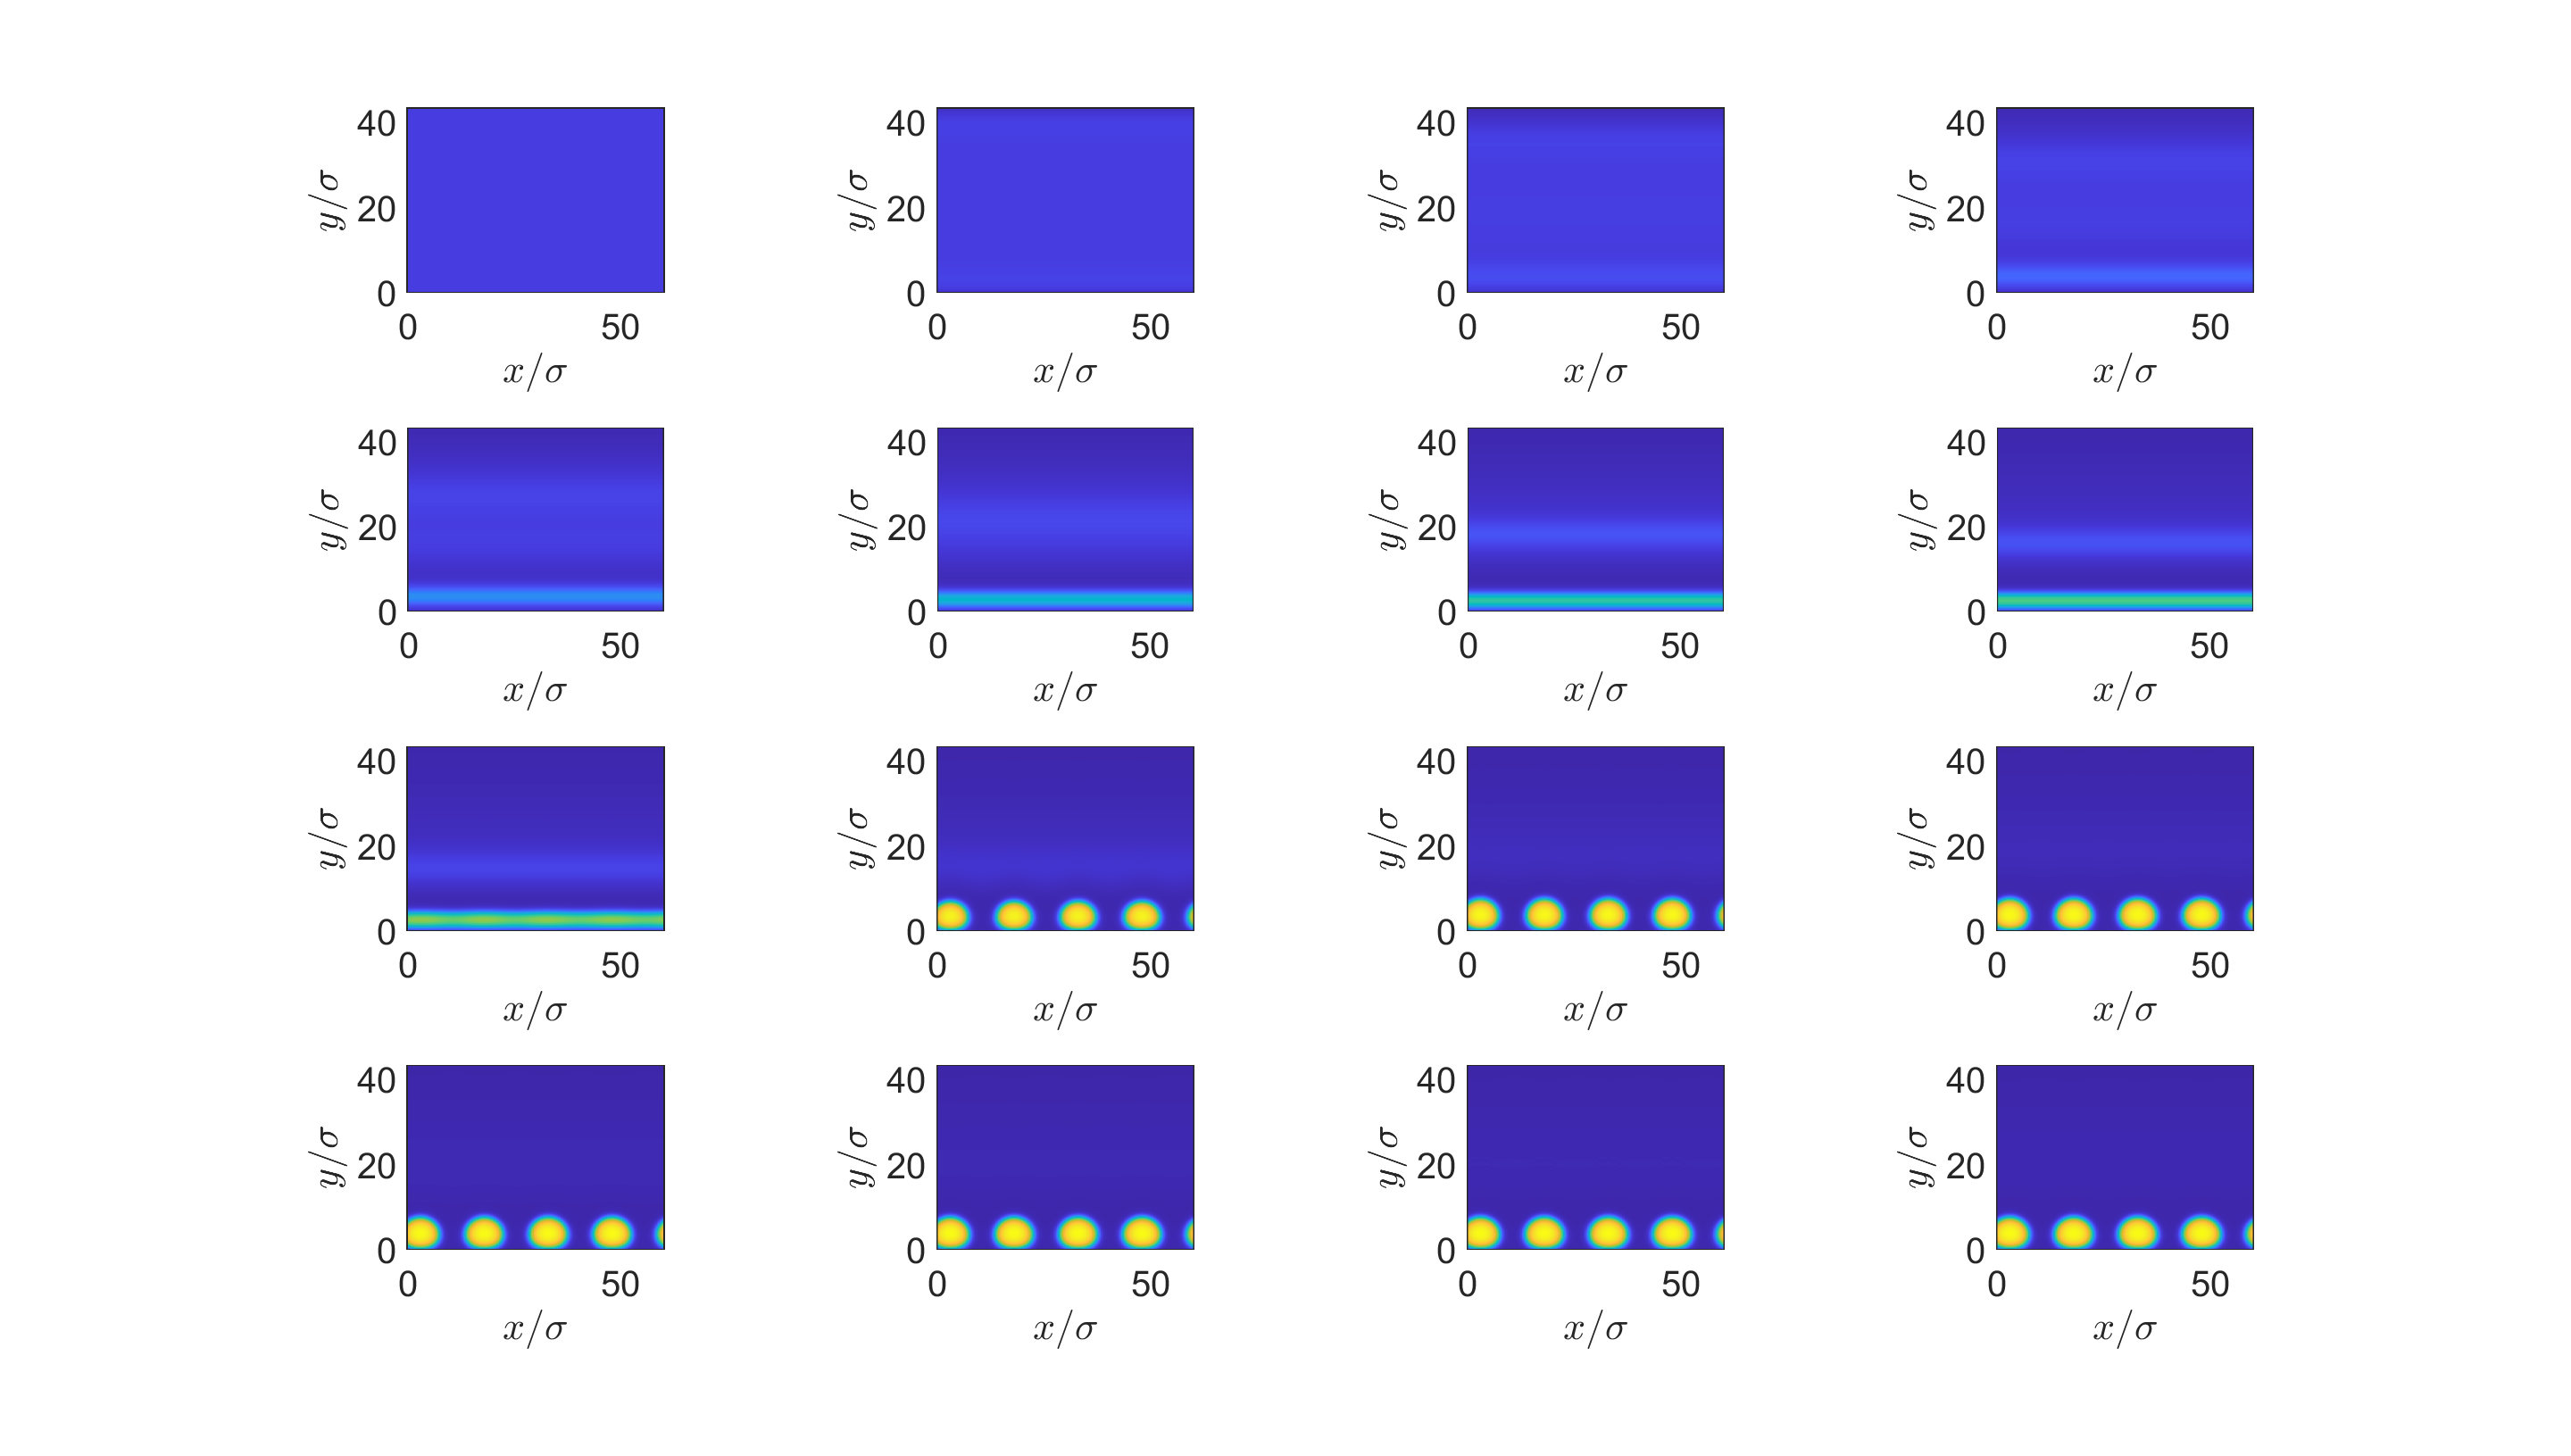
\includegraphics[scale=0.2]{Plotrhobar0072.png}
	\caption{Figure 8 in paper, periodic domain} 
	\label{F5}
\end{figure}
\begin{figure}[h]
	\centering
	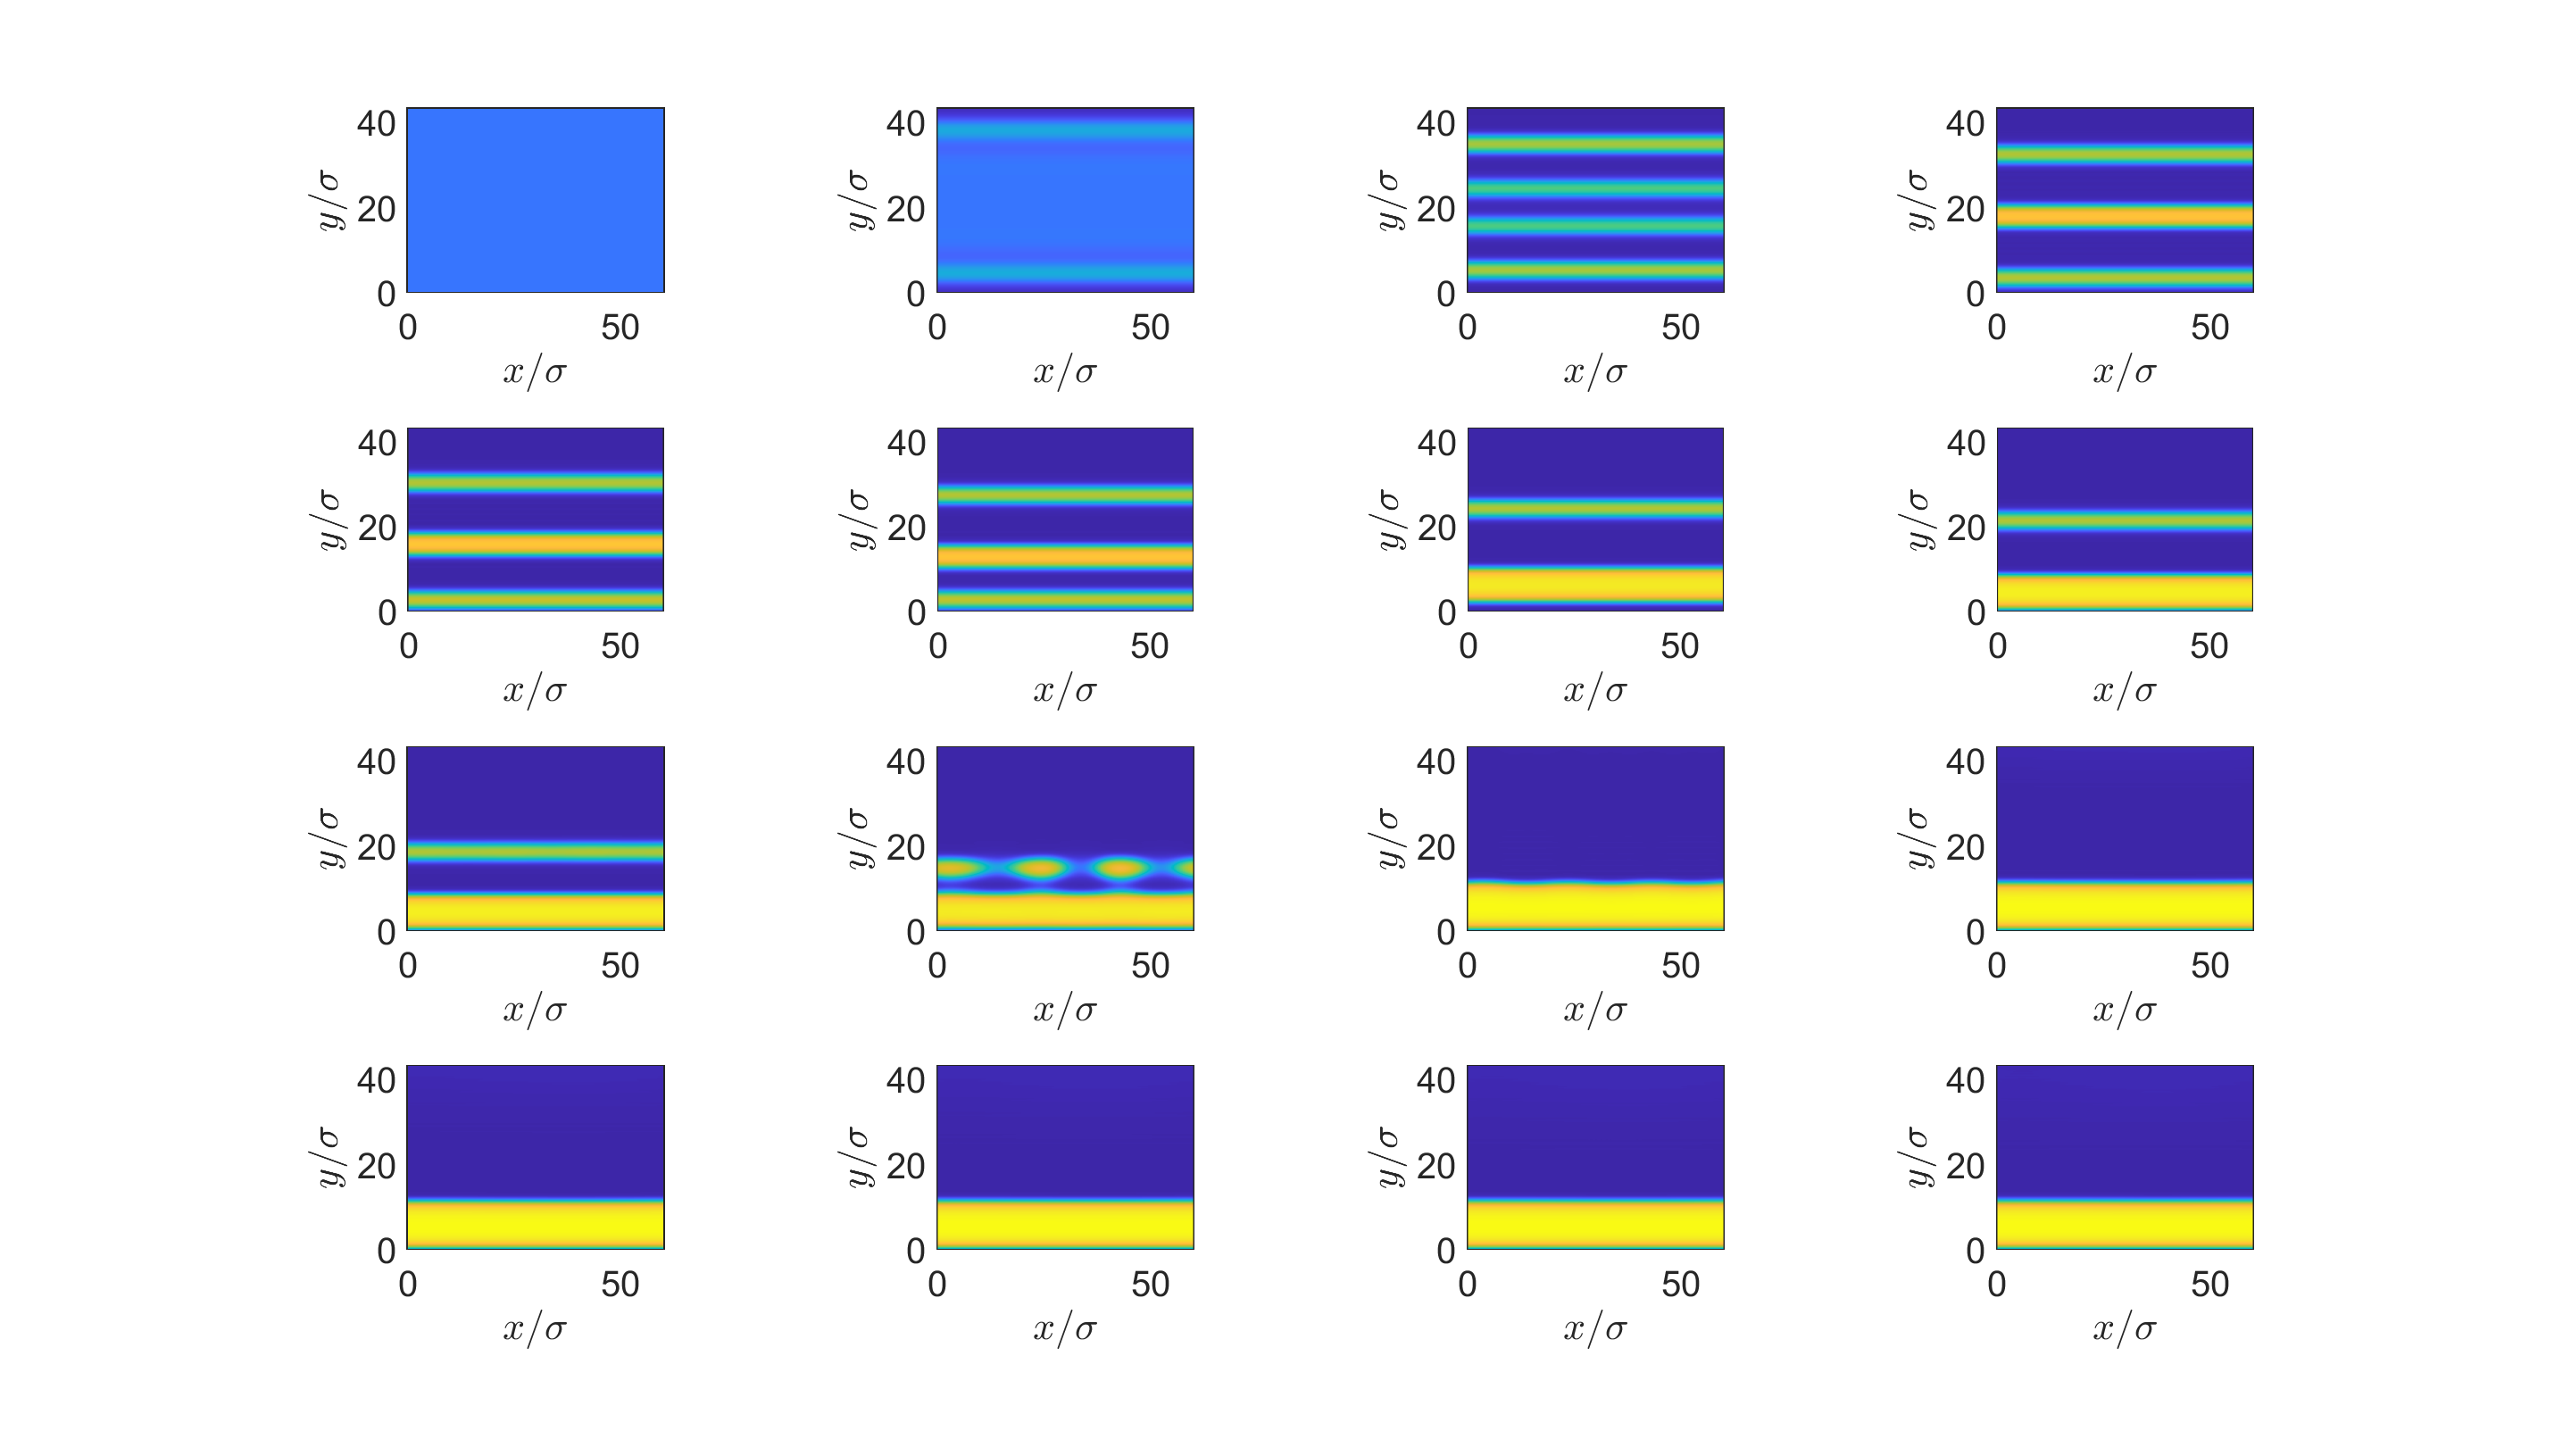
\includegraphics[scale=0.2]{Plotrhobar02.png}
	\caption{Figure 10 in paper, periodic domain} 
	\label{F7}
\end{figure}



\subsubsection{Replicating examples from the paper in a box with noflux BCs}
As above, we choose $N = n = 100$, which takes over 24 hours to run. We run up to time $T = 300$, set $\sigma = 1$ and consider the case $\bar \rho = 0.072$ and $ \bar \rho = 0.2$. Note: the dimensions are switched around, which needs to be fixed with the next rerun. We can see the results for both choices of $\bar \rho$ in Figures \ref{F5b} and \ref{F7b}.

\begin{figure}[h]
	\centering
	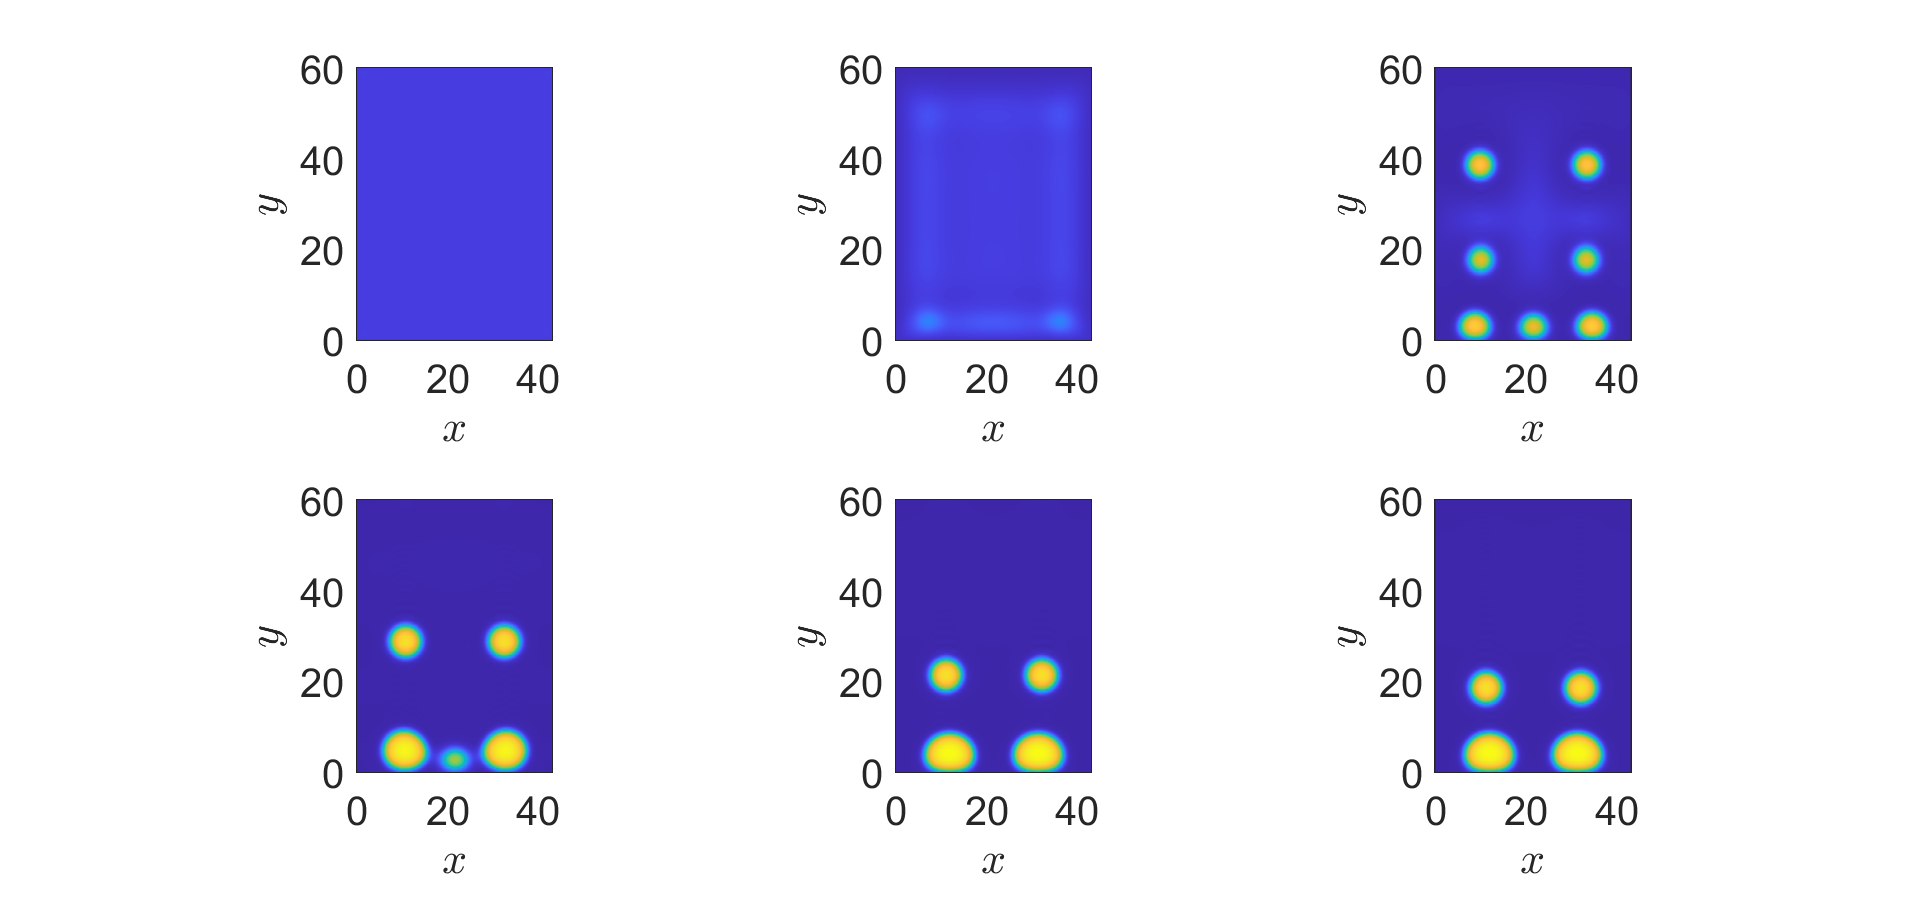
\includegraphics[scale=0.2]{FW0072.png}
	\caption{Figure 8 in paper, no flux BCs, ++ fix wrong dimensions ++} 
	\label{F5b}
\end{figure}
\begin{figure}[h]
	\centering
	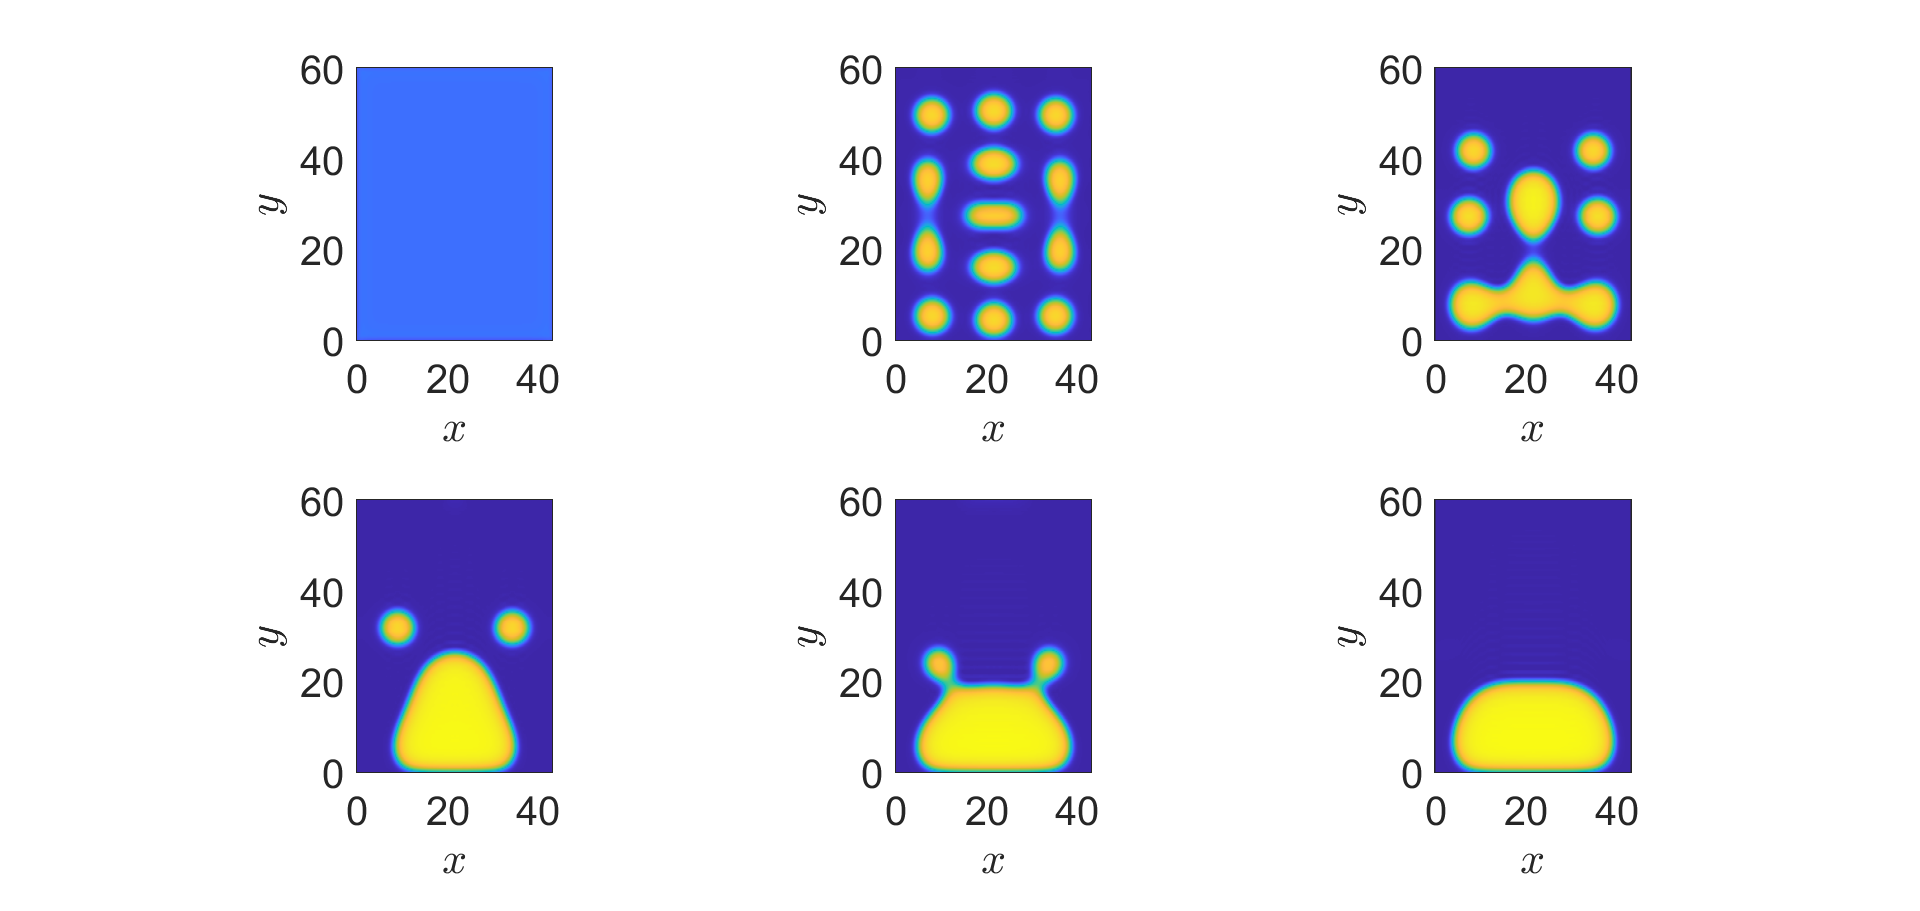
\includegraphics[scale=0.35]{FW02.png}
	\caption{Figure 10 in paper, no flux BCs, ++ fix wrong dimensions ++} 
	\label{F7b}
\end{figure}

	\subsubsection{Optimization in a Box}
We have $N = 40$ and $n = 30$. We choose the ODE tolerance to be $10^{-7}$ and the optimization tolerance is $10^{-3}$. We choose $\bar \rho = 0.036$.
We set up a test problem which sets $\hr$ to be the forward solution for the problem with $V_{ext} = cy$, where $c = 0.1$, as in Archer's paper. The optimization forward problem is such that $c = 0.01$ and $\w = \mathbf 0$. We expect the control to act downward, since the strength of gravity $c$ is decreased.
We also expect that the cost $\mathcal J$ is decreasing from the baseline $J_{FW}$ when optimizing.
For $\beta = 10^{-3}$ and $\beta = 10^{-1}$ this works well.
When $\beta = 10^{-3}$ we get $J_{FW} = 0.4955$ and $J_{Opt} = 0.0556 $. 
The results can be seen in Figures \ref{Fa1}, \ref{Fa2} and \ref{Fa3}.
\begin{figure}[h]
	\centering
	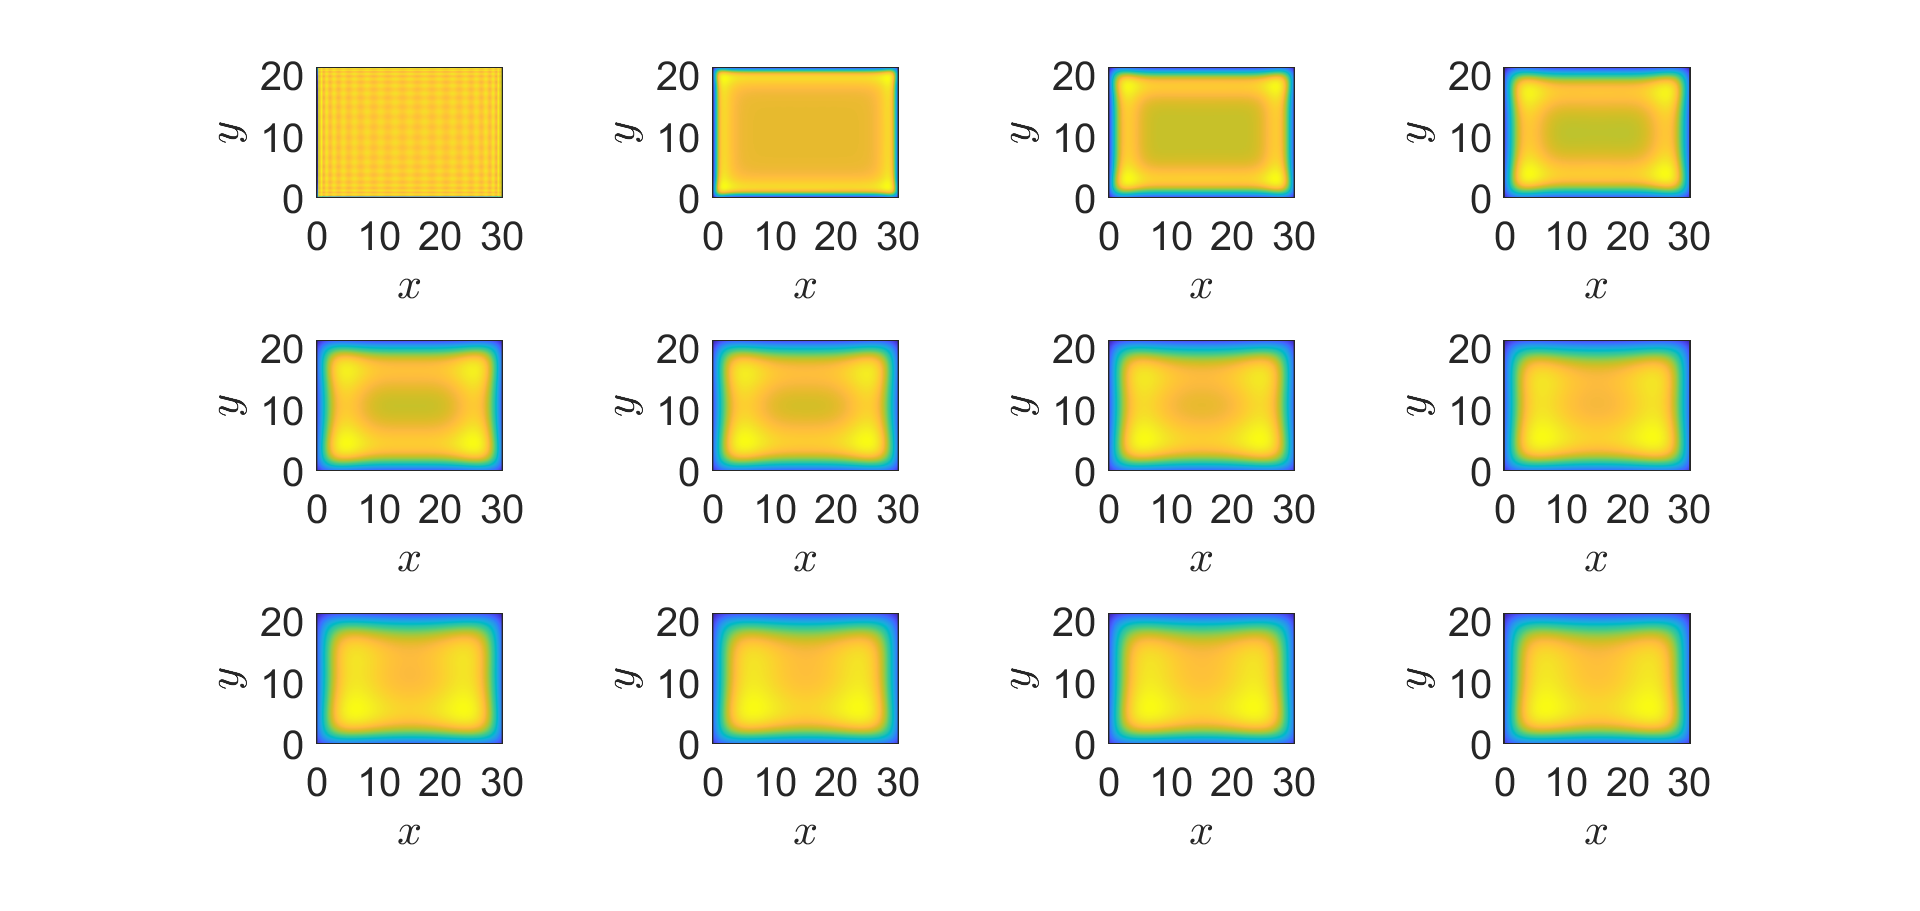
\includegraphics[scale=0.35]{F11.png}
	\caption{Forward $\rho$ for $c = 0.01$} 
	\label{Fa1}
\end{figure}	
\begin{figure}[h]
	\centering
	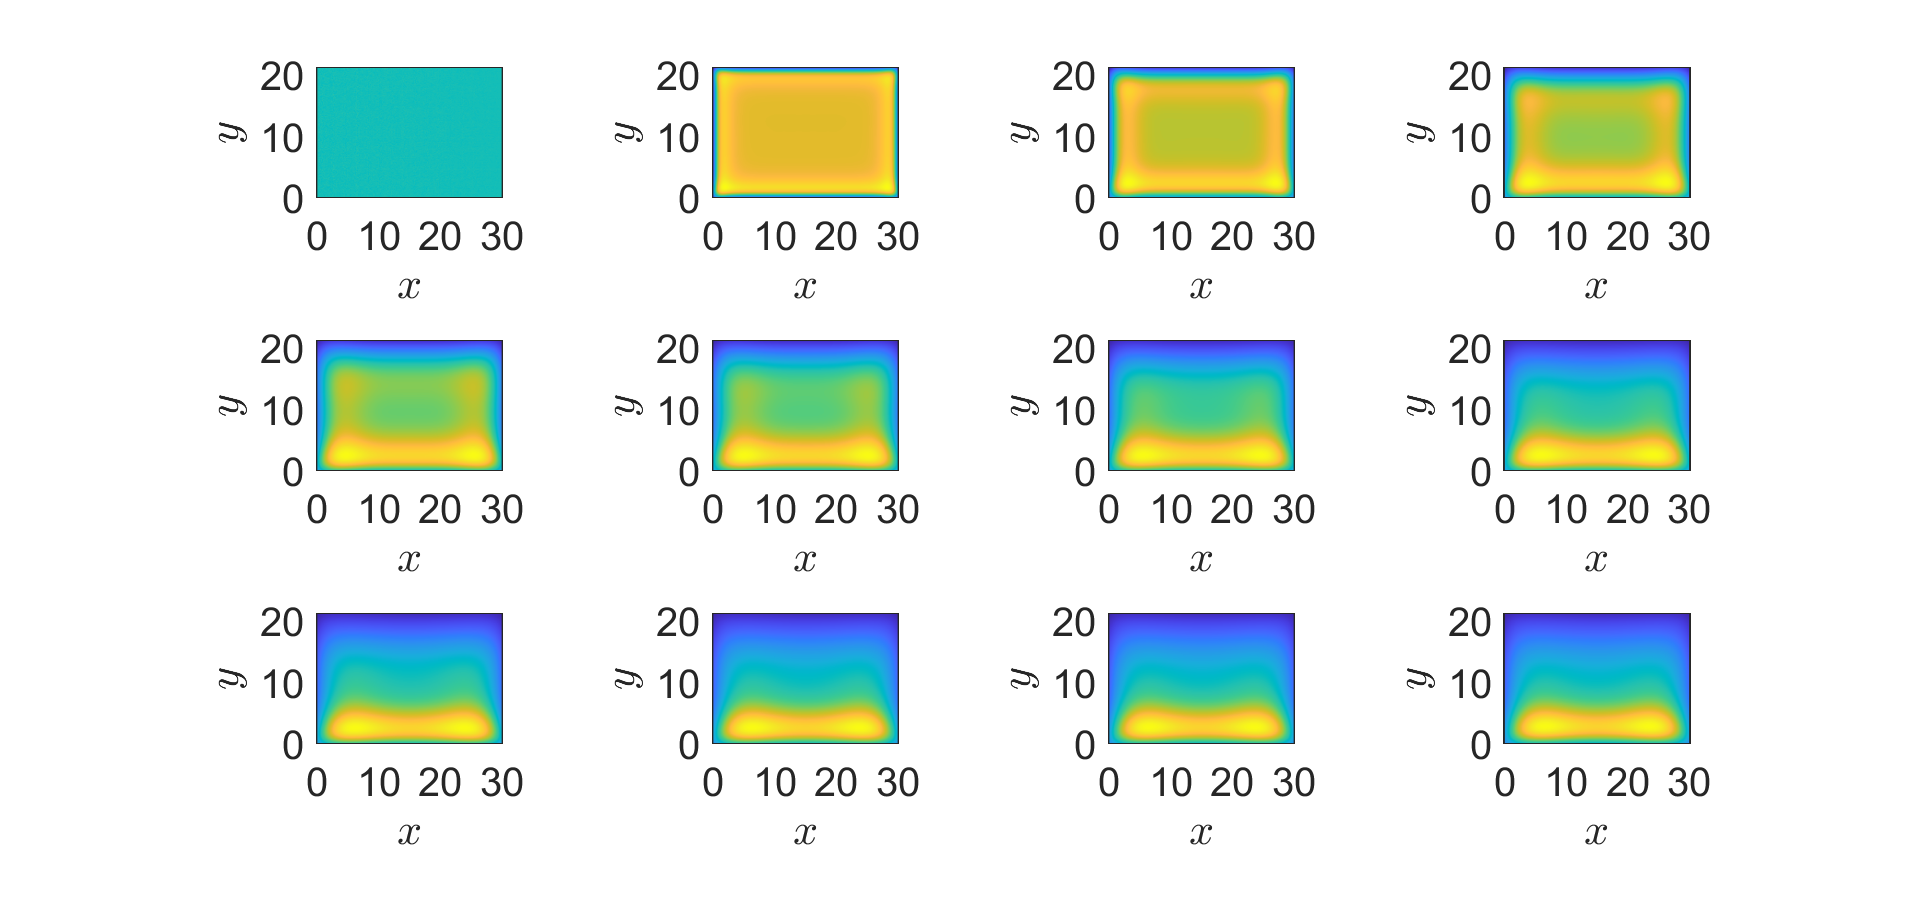
\includegraphics[scale=0.35]{F21.png}
	\caption{Optimal $\rho$ for $c = 0.01$} 
	\label{Fa2}
\end{figure}
\begin{figure}[h]
	\centering
	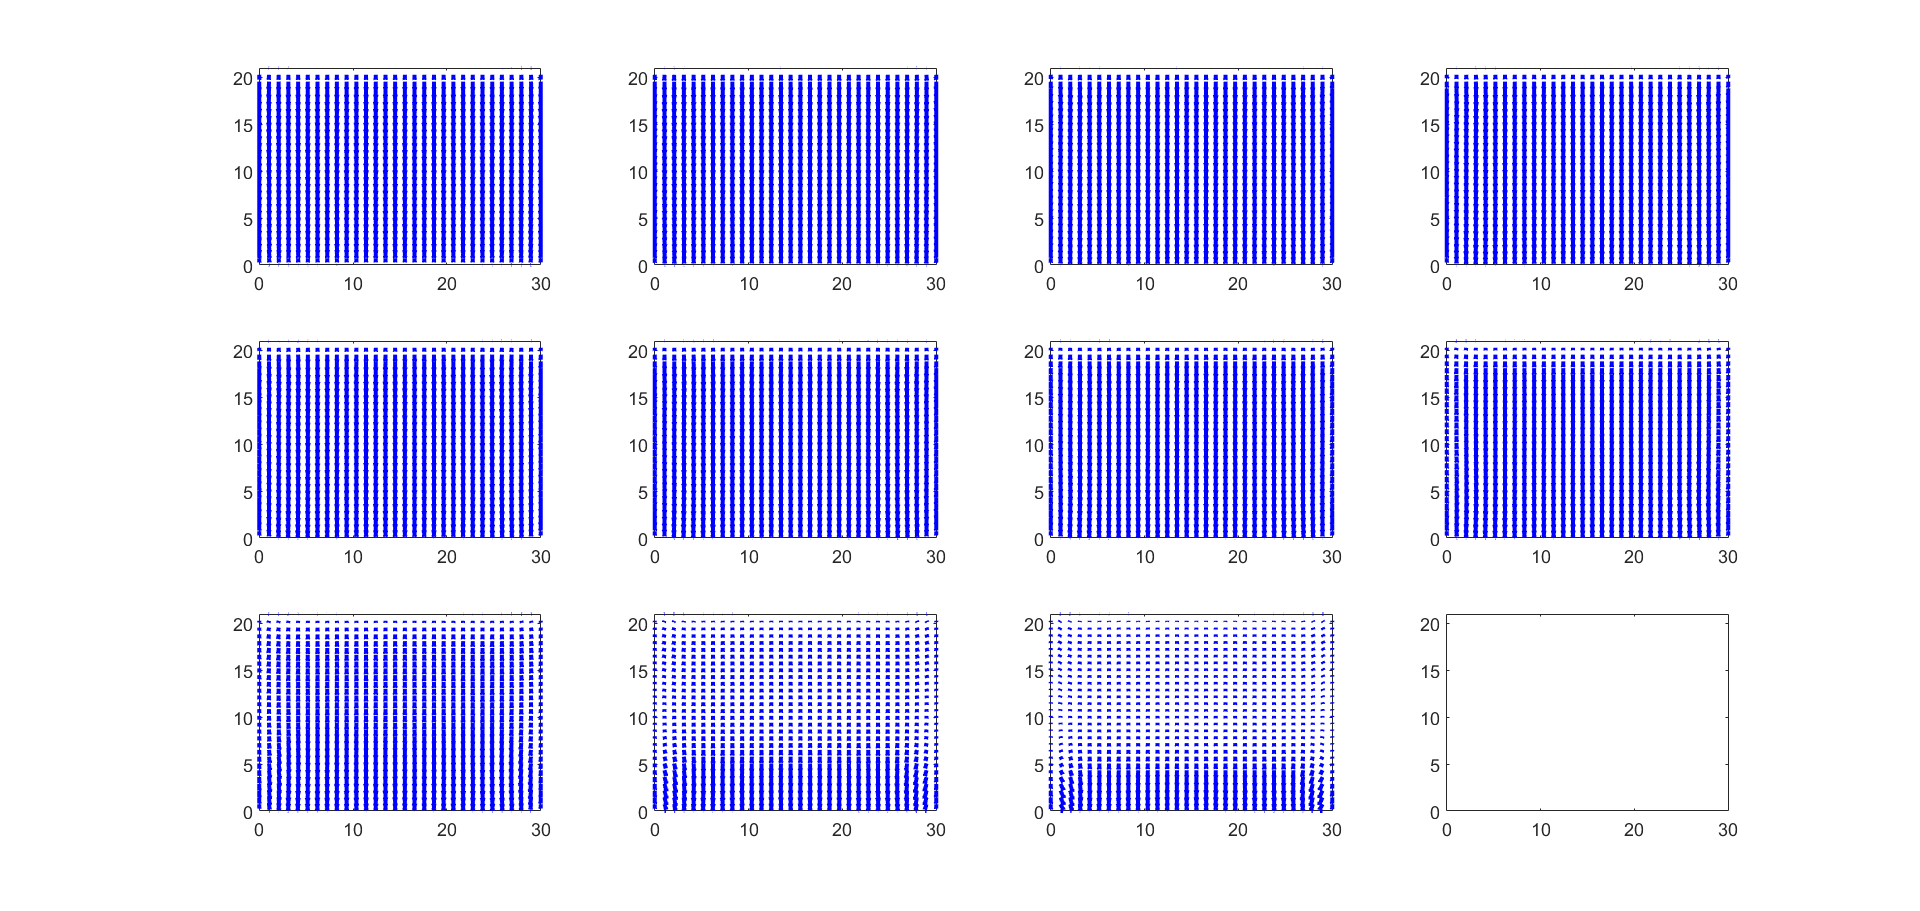
\includegraphics[scale=0.35]{F31.png}
	\caption{Optimal Control for $c = 0.01$} 
	\label{Fa3}
\end{figure}



\subsubsection{Optimization in a Box - Time-Independent Control}
We consider the identical problem but now require the control to be time independent. This affects the gradient equation as discussed in Section \ref{sec:TimeIndependentControl}.
Therefore, we expect a $\w$ which is averaged over the time horizon and therefore time independent. The result is $J_{FW} = 0.4855$ and $J_{Opt} = 0.0733$ and can be seen in Figures \ref{F6a}, \ref{F7a} and \ref{F8a}. We observe that, as expected, $J_{opt}$ is larger than for the previous example where $\w$ was allowed to vary over time.

\begin{figure}[h]
	\centering
	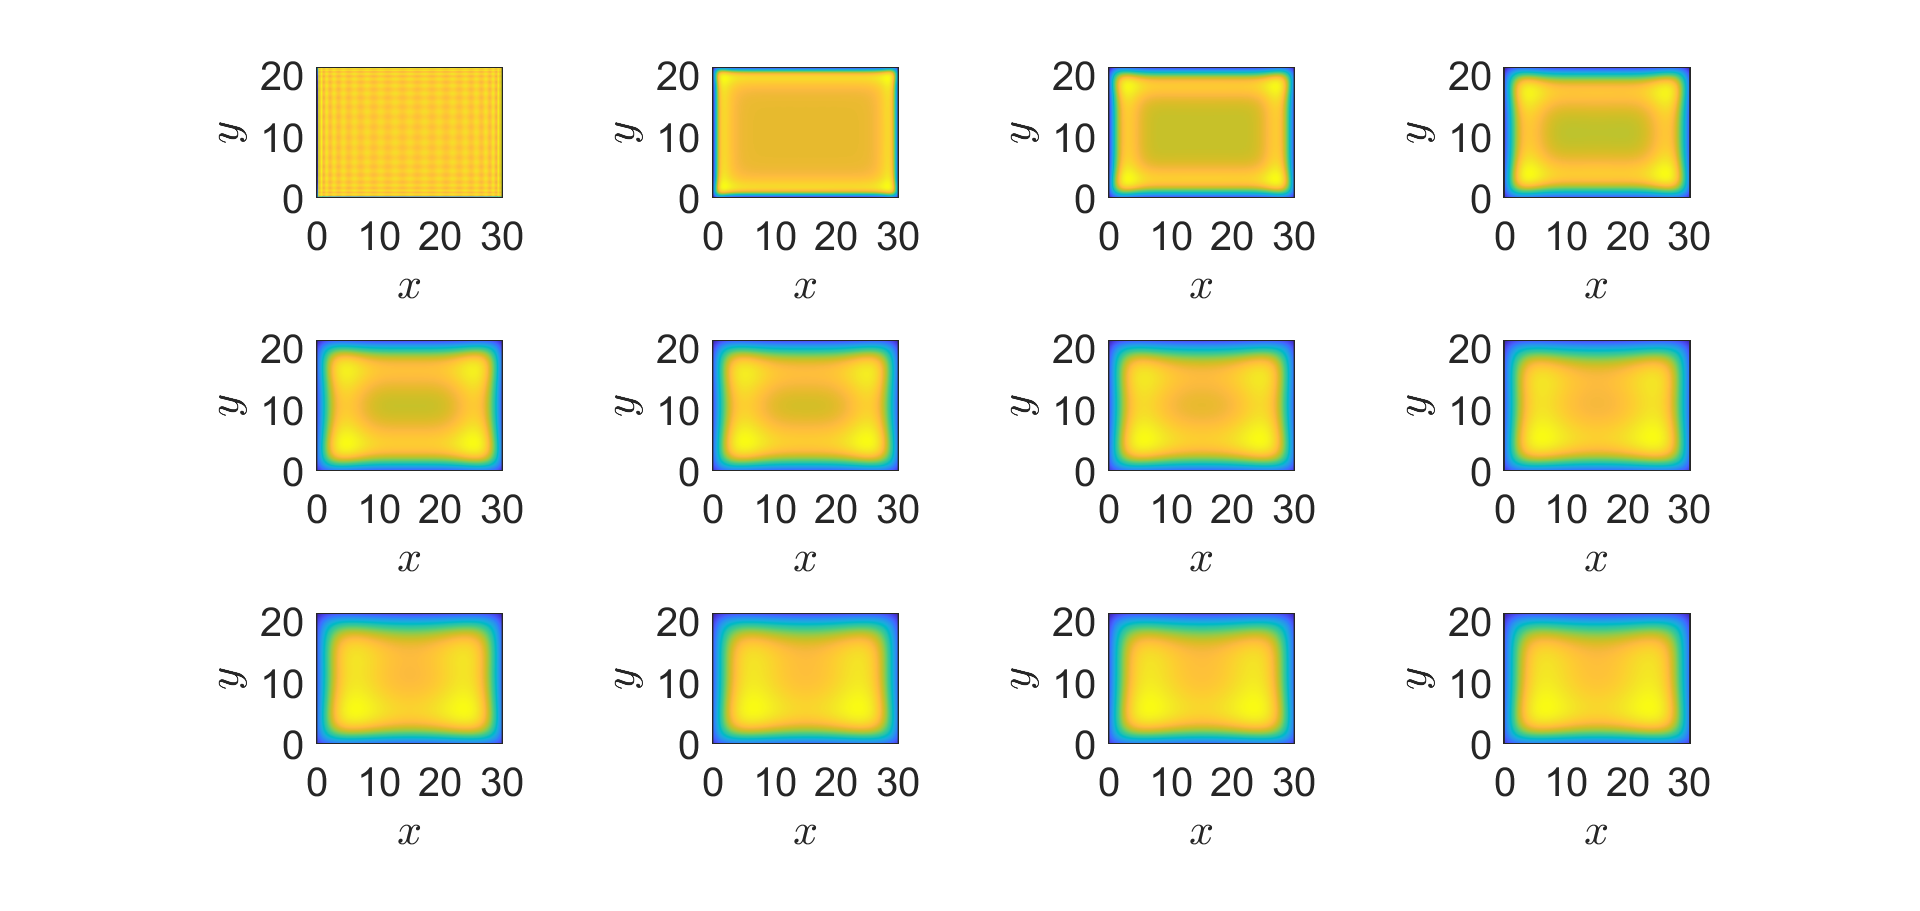
\includegraphics[scale=0.35]{C1.png}
	\caption{Time-independent; Forward $\rho$ for $a = 0.01$} 
	\label{F6a}
\end{figure}	
\begin{figure}[h]
	\centering
	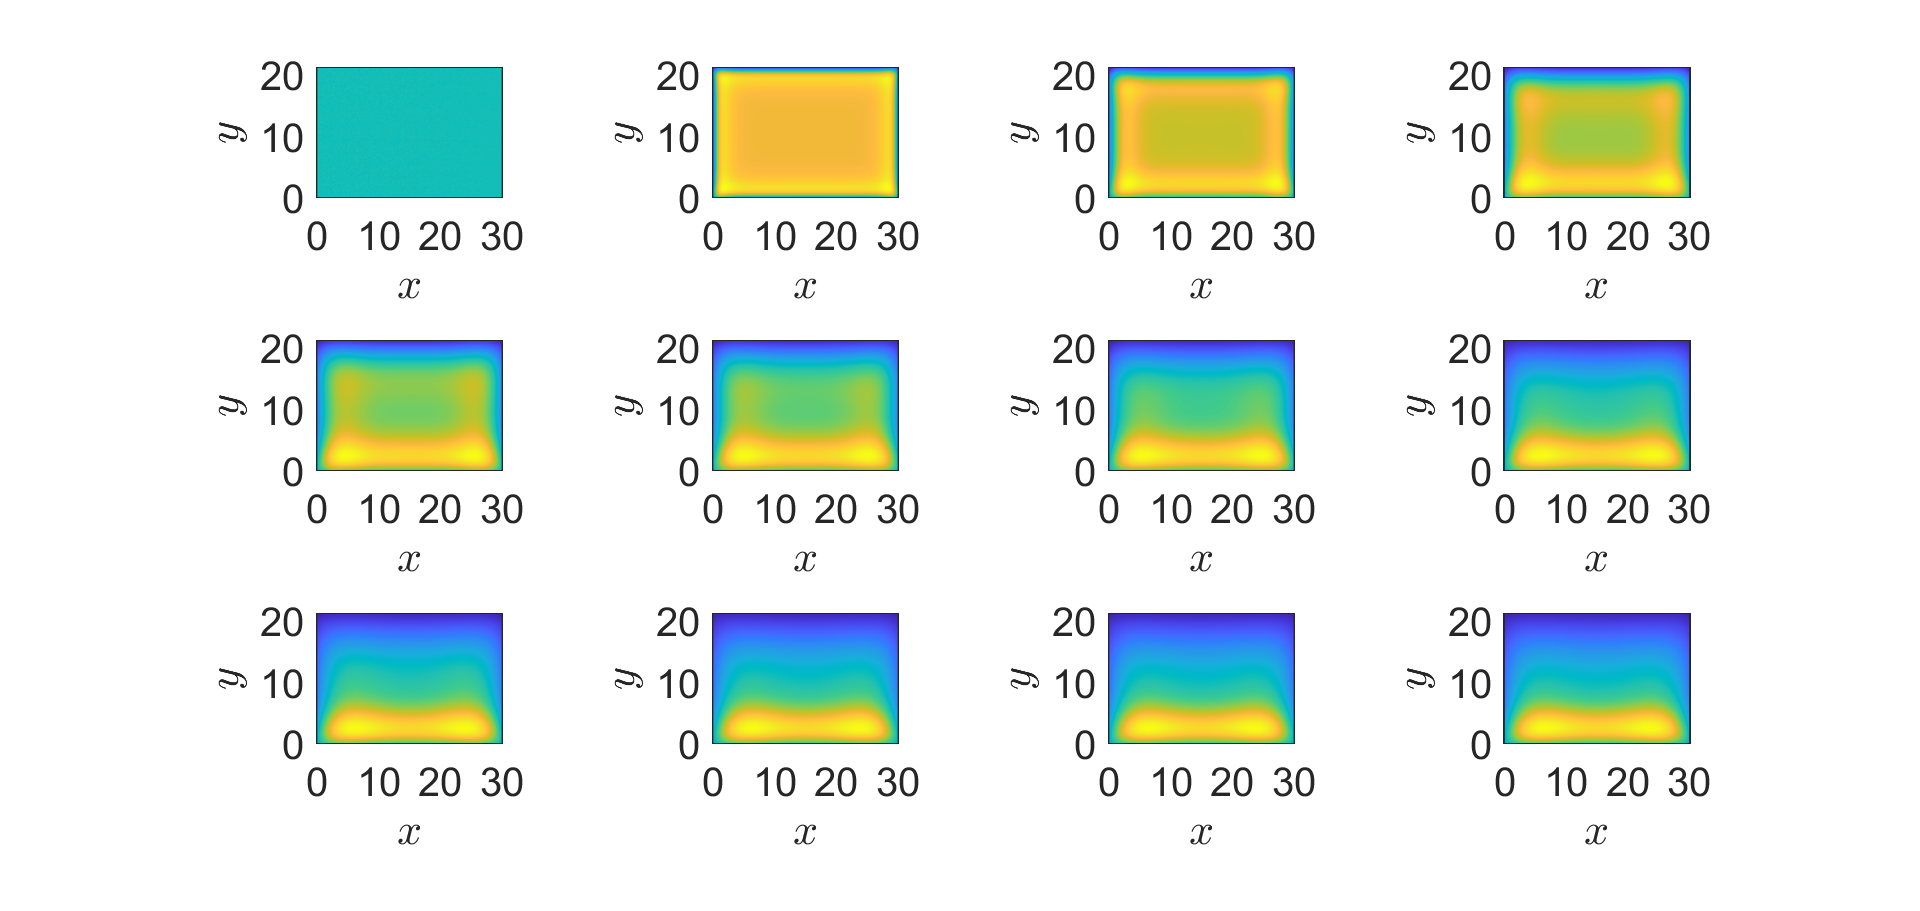
\includegraphics[scale=0.35]{C2.png}
	\caption{Time-independent; Optimal $\rho$ for $a = 0.01$} 
	\label{F7a}
\end{figure}
\begin{figure}[h]
	\centering
	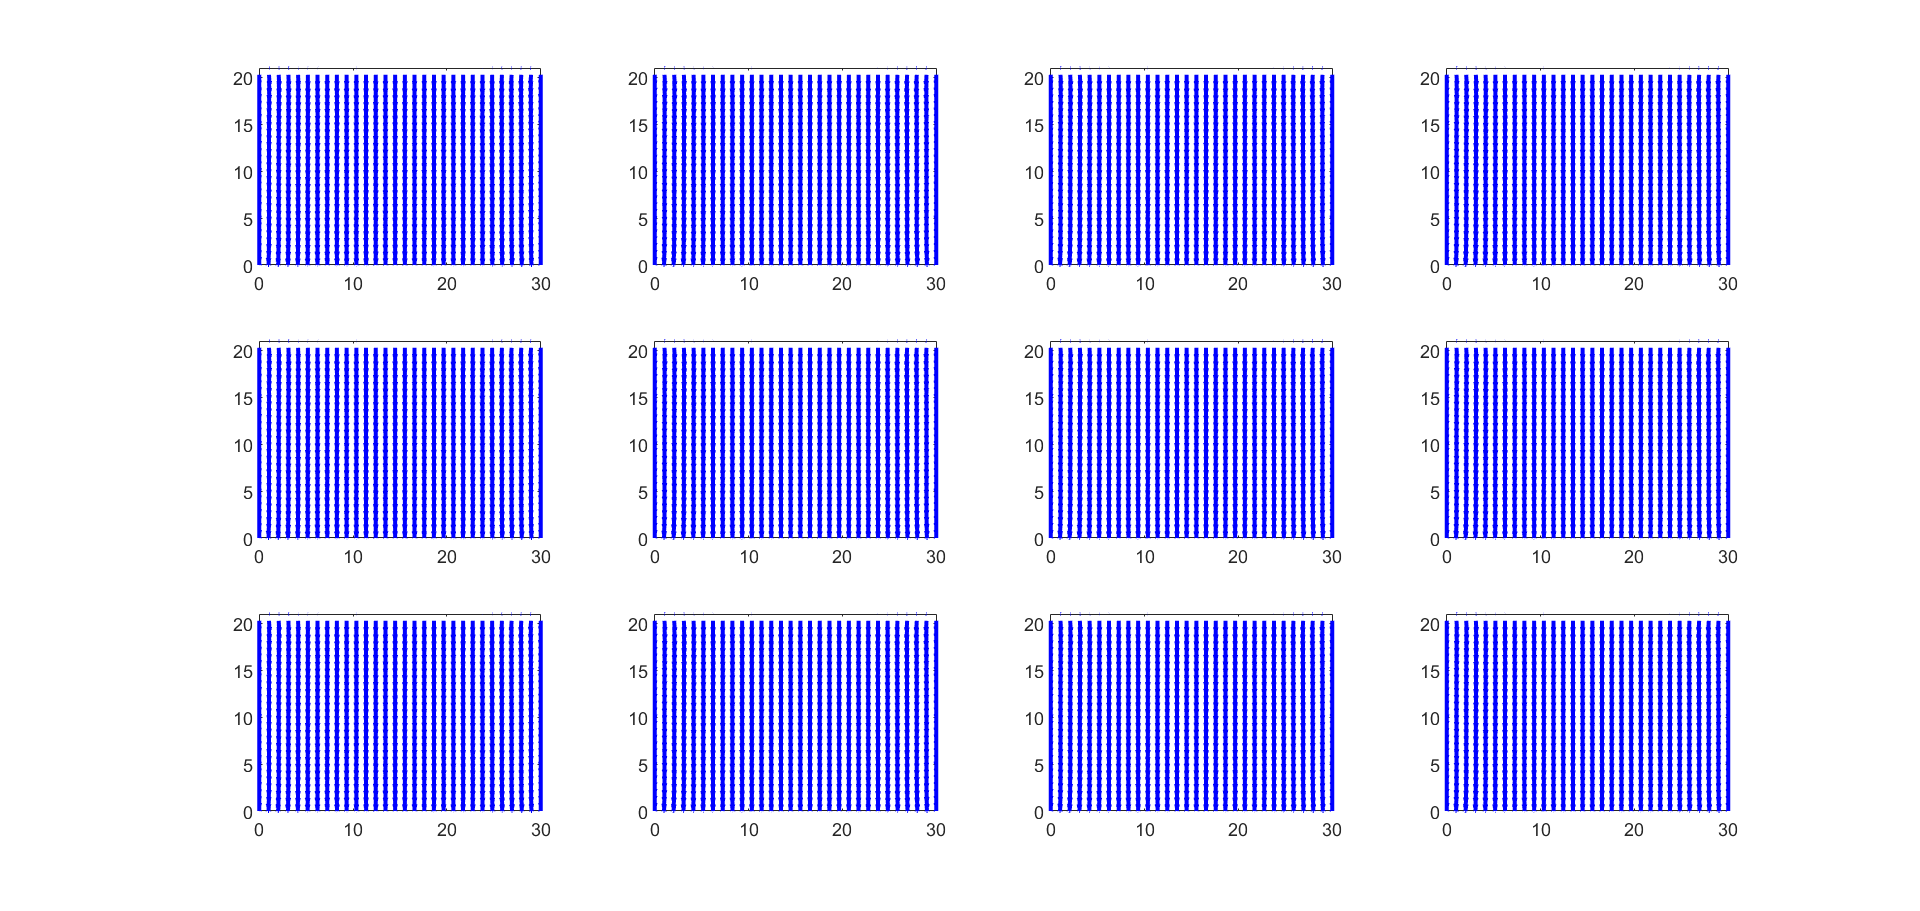
\includegraphics[scale=0.35]{C3.png}
	\caption{Time-independent; Optimal Control for $a = 0.01$} 
	\label{F8a}
\end{figure}

We wanted to see whether the time independent flow control is similar to the $\nabla V_{ext}$ of the target.
The target state was influenced by $V_{ext} = 0.1 y_2$. The forward state for the OCP was influenced by $V_{ext} = 0.01 y_2$. 
Figure \ref{F1a} shows the control and $\nabla V_{ext}$ of the target. We can see that one of these is positive, while the other one is negative. This is due to the opposite signs of $\w$ and $\nabla V_{ext}$ in the PDE.

\begin{figure}[h]
	\centering
	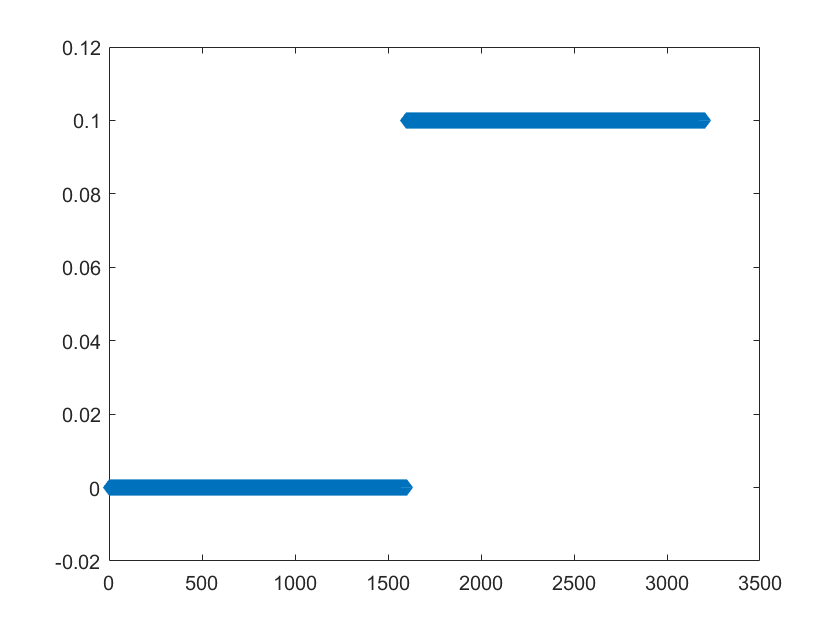
\includegraphics[scale=0.35]{V1.png}
	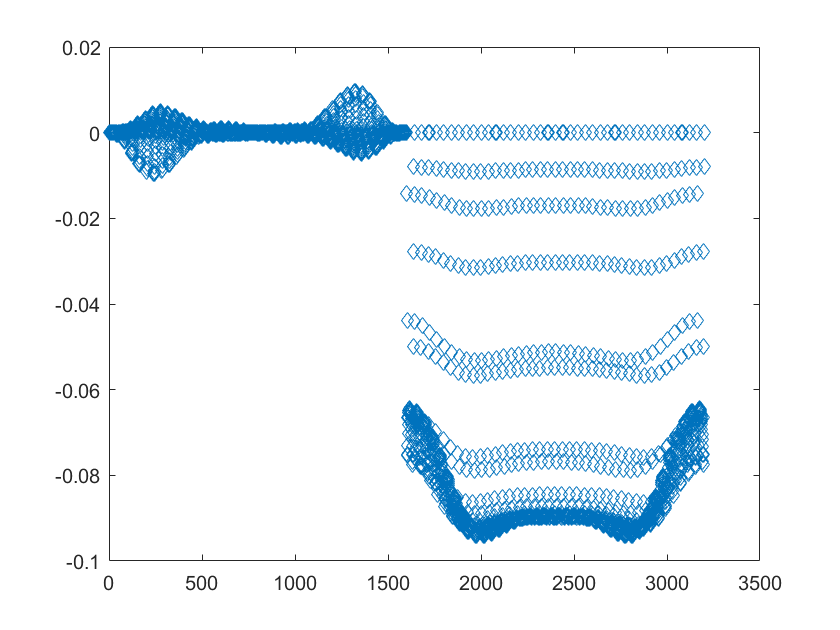
\includegraphics[scale=0.35]{W1.png}
	\caption{$\nabla V_{ext}$ of target and optimal control $\w$.} 
	\label{F1a}
\end{figure}

\subsubsection{Optimization in a Periodic Box}

\subsubsection{Optimization in a Periodic Box - Time-Independent Control}

\subsubsection{Optimization in a Multishape}
The first example is a simple mulitshape with two quadrilaterals. We choose $n = 30$ and $N = 20$ and run up to time $T = 30$, the parameter choices are as in the section on optimization in a box. We choose $\lambda = 0.01$ as usual. We get $J_{FW} = 0.0713$ and $J_{Opt} = 0.0059$. The results are displayed in Figures \ref{FM0} and \ref{FM0a}.
\begin{figure}[h]
	\centering
	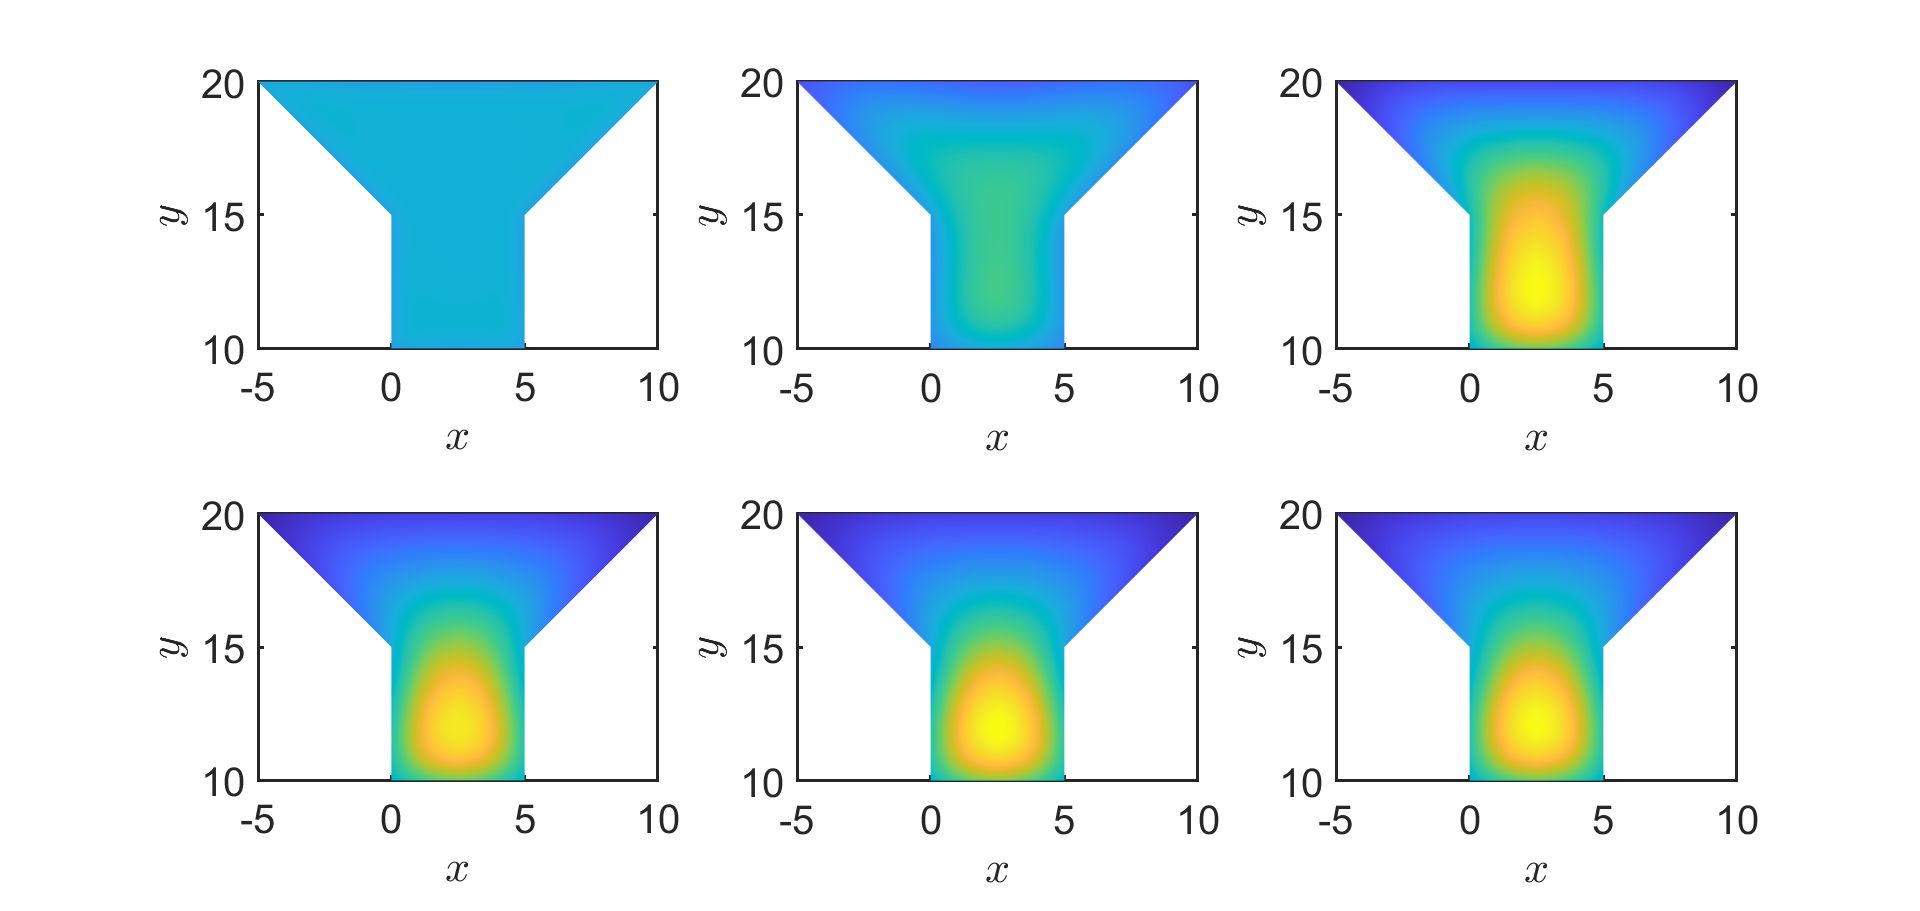
\includegraphics[scale=0.35]{MultiOpt1a.png}
	\caption{Multishape Example 1: Optimal $\rho$} 
	\label{FM0}
\end{figure}
\begin{figure}[h]
	\centering
	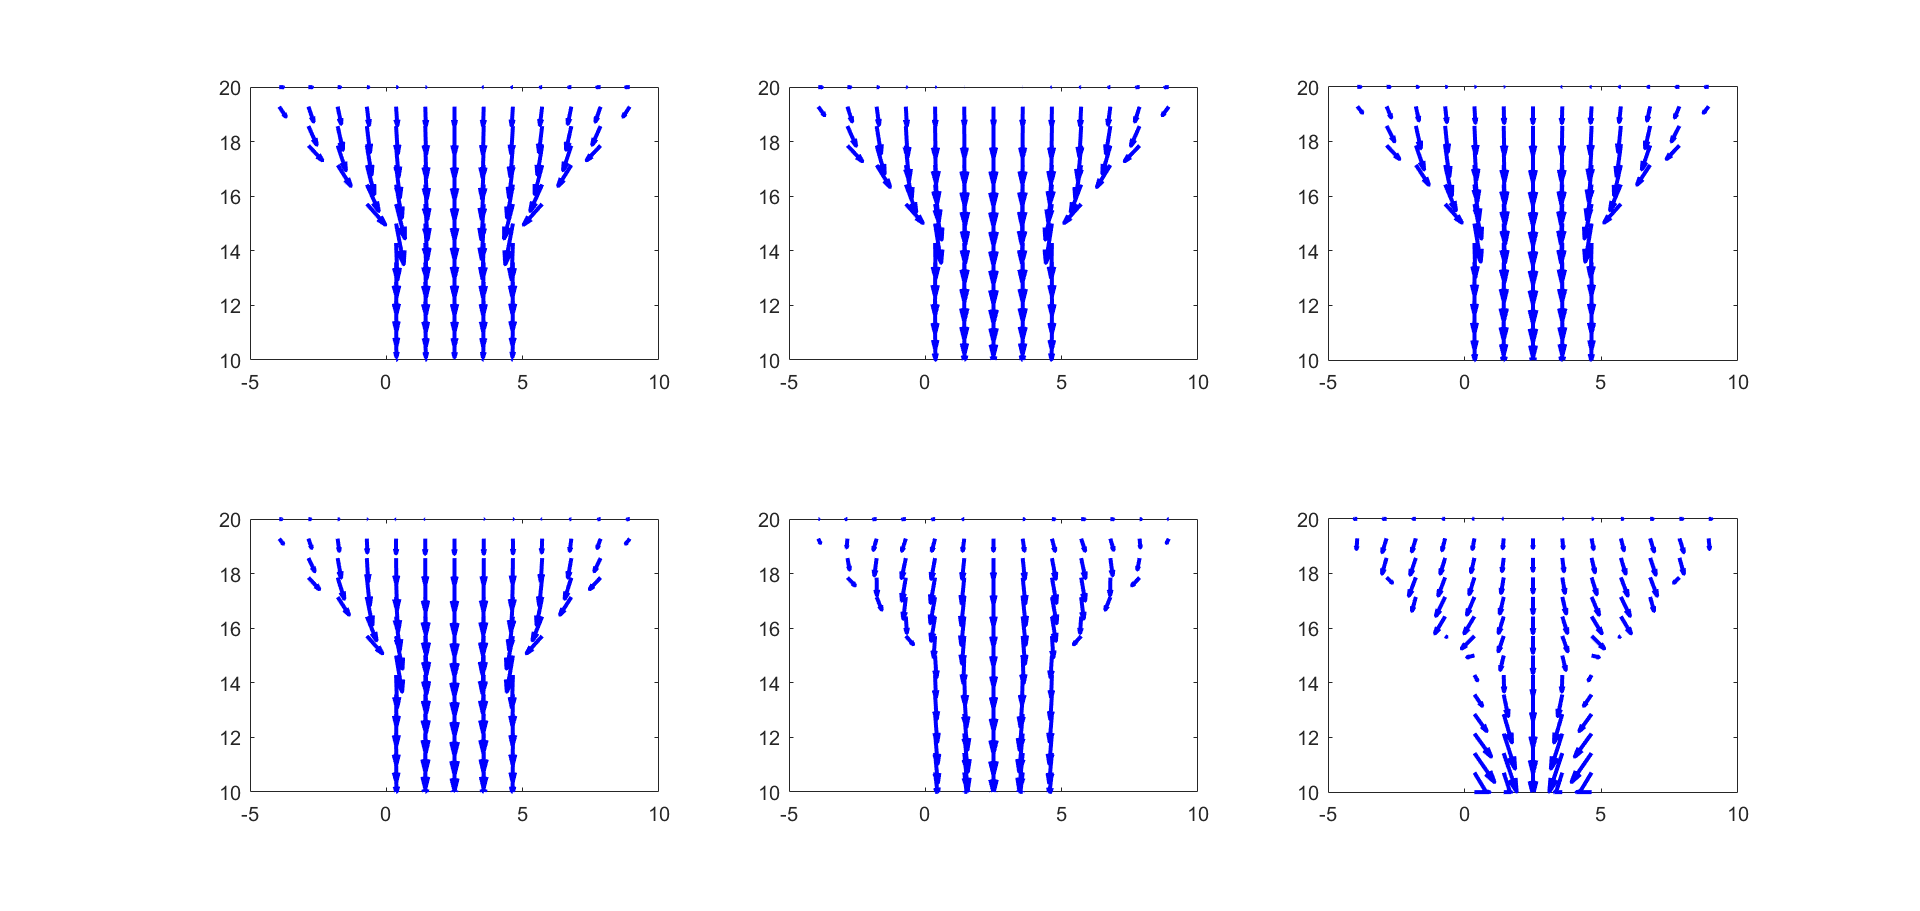
\includegraphics[scale=0.35]{MultiCont1a.png}
	\caption{Multishape Example 1: Optimal control} 
	\label{FM0a}
\end{figure}
\\
\\
The second example is an optimization problem in a larger multishape. The setup remains the same as before, but now computed on a multishape which is comprised of four shapes, out of which three are quadrilaterals and one is a wedge. We get $J_{FW} = 0.0766$ and $J_{Opt} = 0.0116$. The results can be seen in Figures \ref{FM1a} and \ref{FM2a}.
\begin{figure}[h]
	\centering
	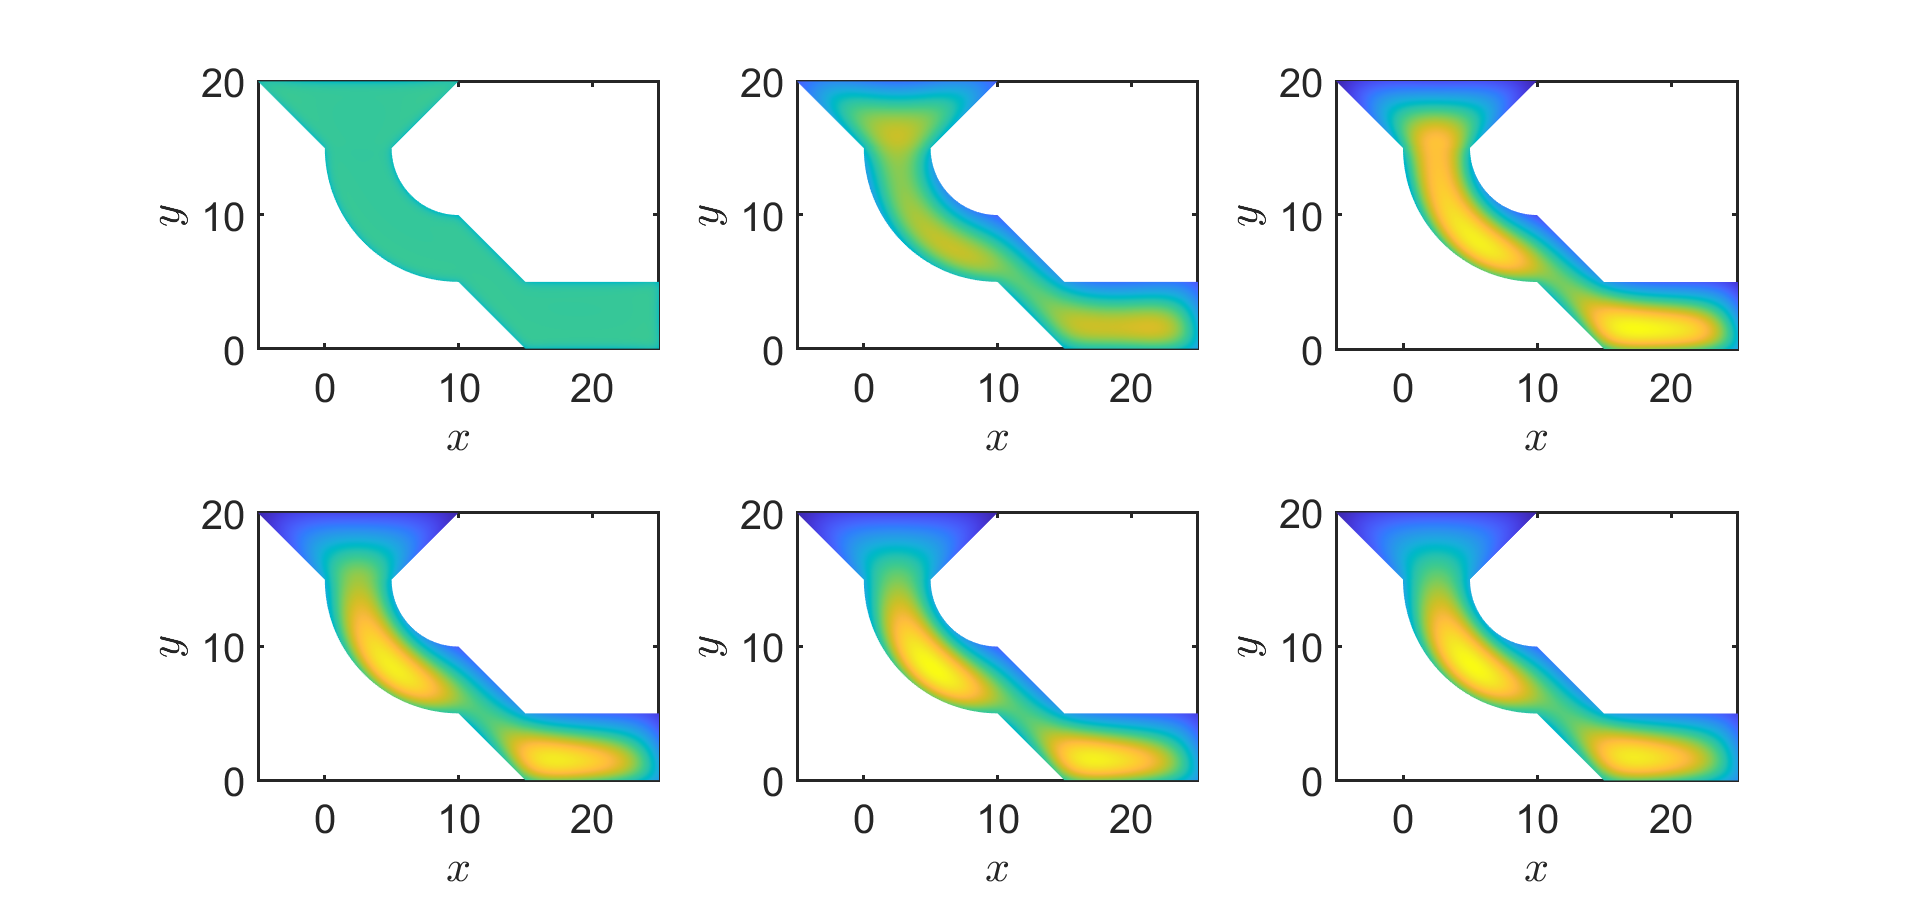
\includegraphics[scale=0.35]{MultiOpt2.png}
	\caption{Multishape Example 2: Optimal $\rho$} 
	\label{FM1a}
\end{figure}
\begin{figure}[h]
	\centering
	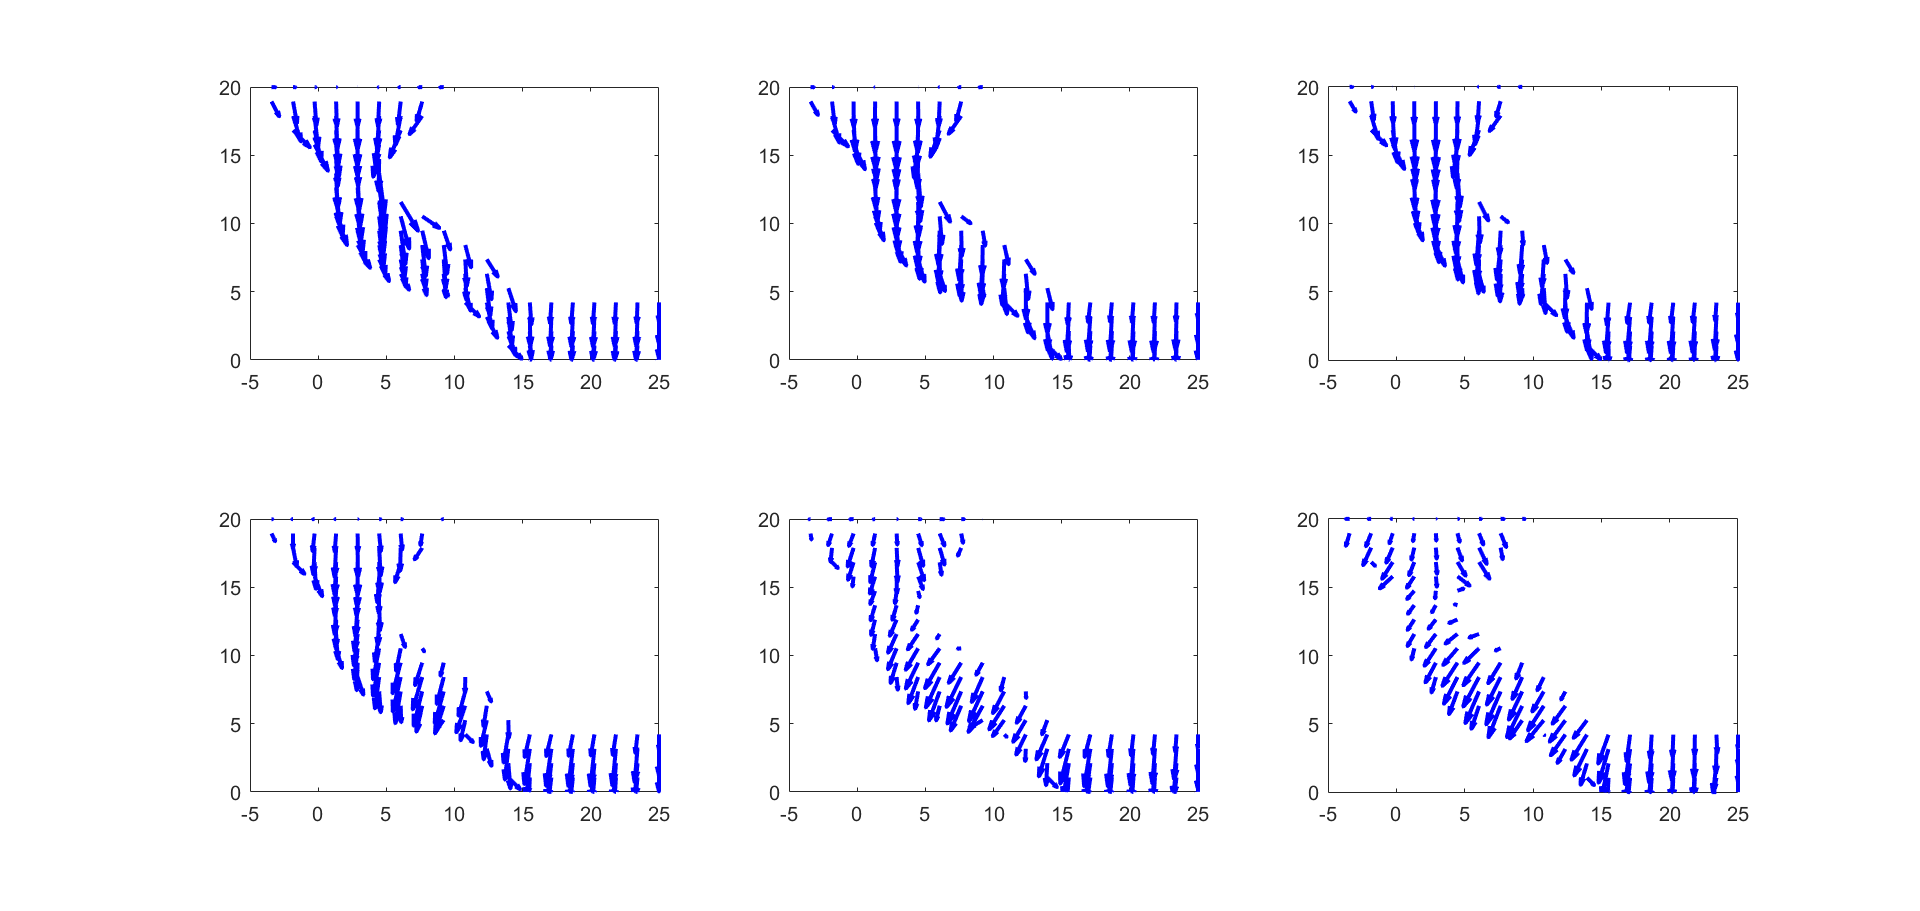
\includegraphics[scale=0.35]{MultiCont2.png}
	\caption{Multishape Example 2: Optimal control} 
	\label{FM2a}
\end{figure}
\\
\\
+++++++++++ I think this is time independent!! ++++++++++++++++++++++++++++
For a third example, we choose a multishape with an imposed background flow and gravity as a target, see Figure \ref{FM3}. The optimal control problem has the same strength of gravity $c = 0.1$ imposed, but no flow. We expect the control to act similar to the flow profile imposed to produce $\hr$. We choose $T = 10$ this time.
We get $J_{FW} = 0.0484$ and $J_{Opt} = 0.0258$ and the results are displayed in Figures \ref{FM3a} and \ref{FM3b}. Furthermore, we compare the strength of $\w$ of the target and the optimal control. The absolute $L_2$/ $L_\infty$ norms are compared, and we get $||\w_{\hr}|| = 68$ and $||\w_{Opt}|| = 50.8965$.
\begin{figure}[h]
	\centering
	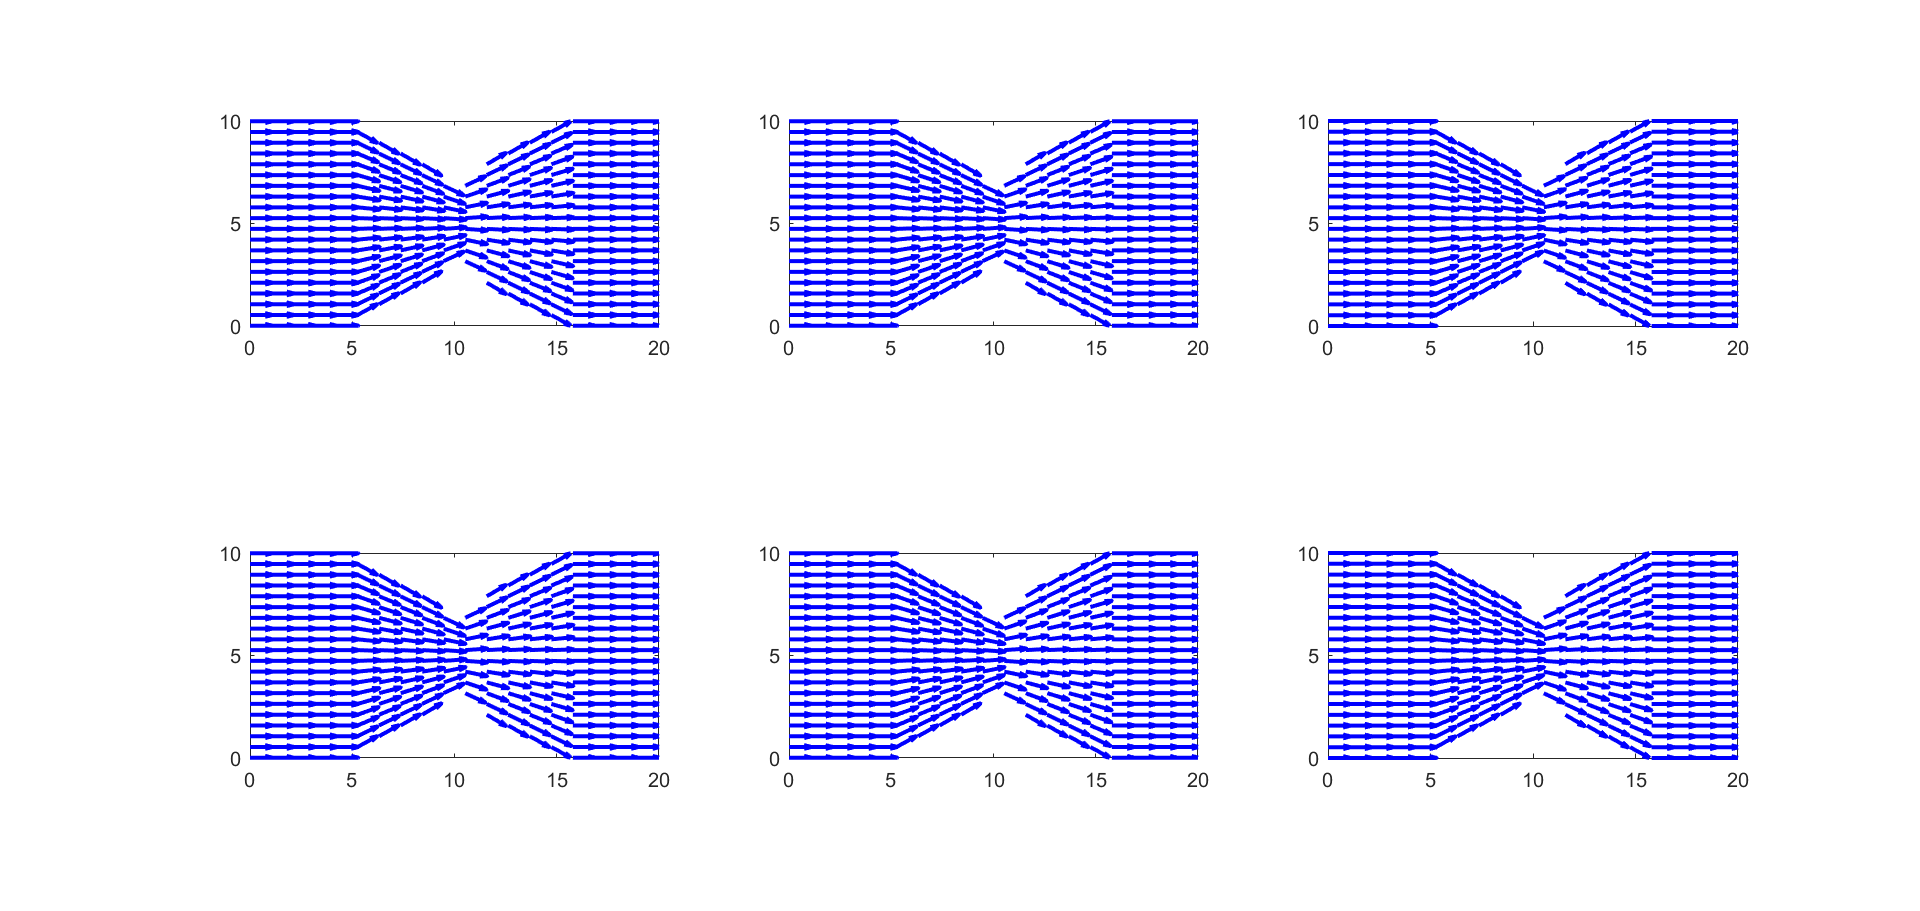
\includegraphics[scale=0.35]{MultiwFW.png}
	\caption{Multishape Example 3:Flow profile determining $\hr$} 
	\label{FM3}
\end{figure}
\begin{figure}[h]
	\centering
	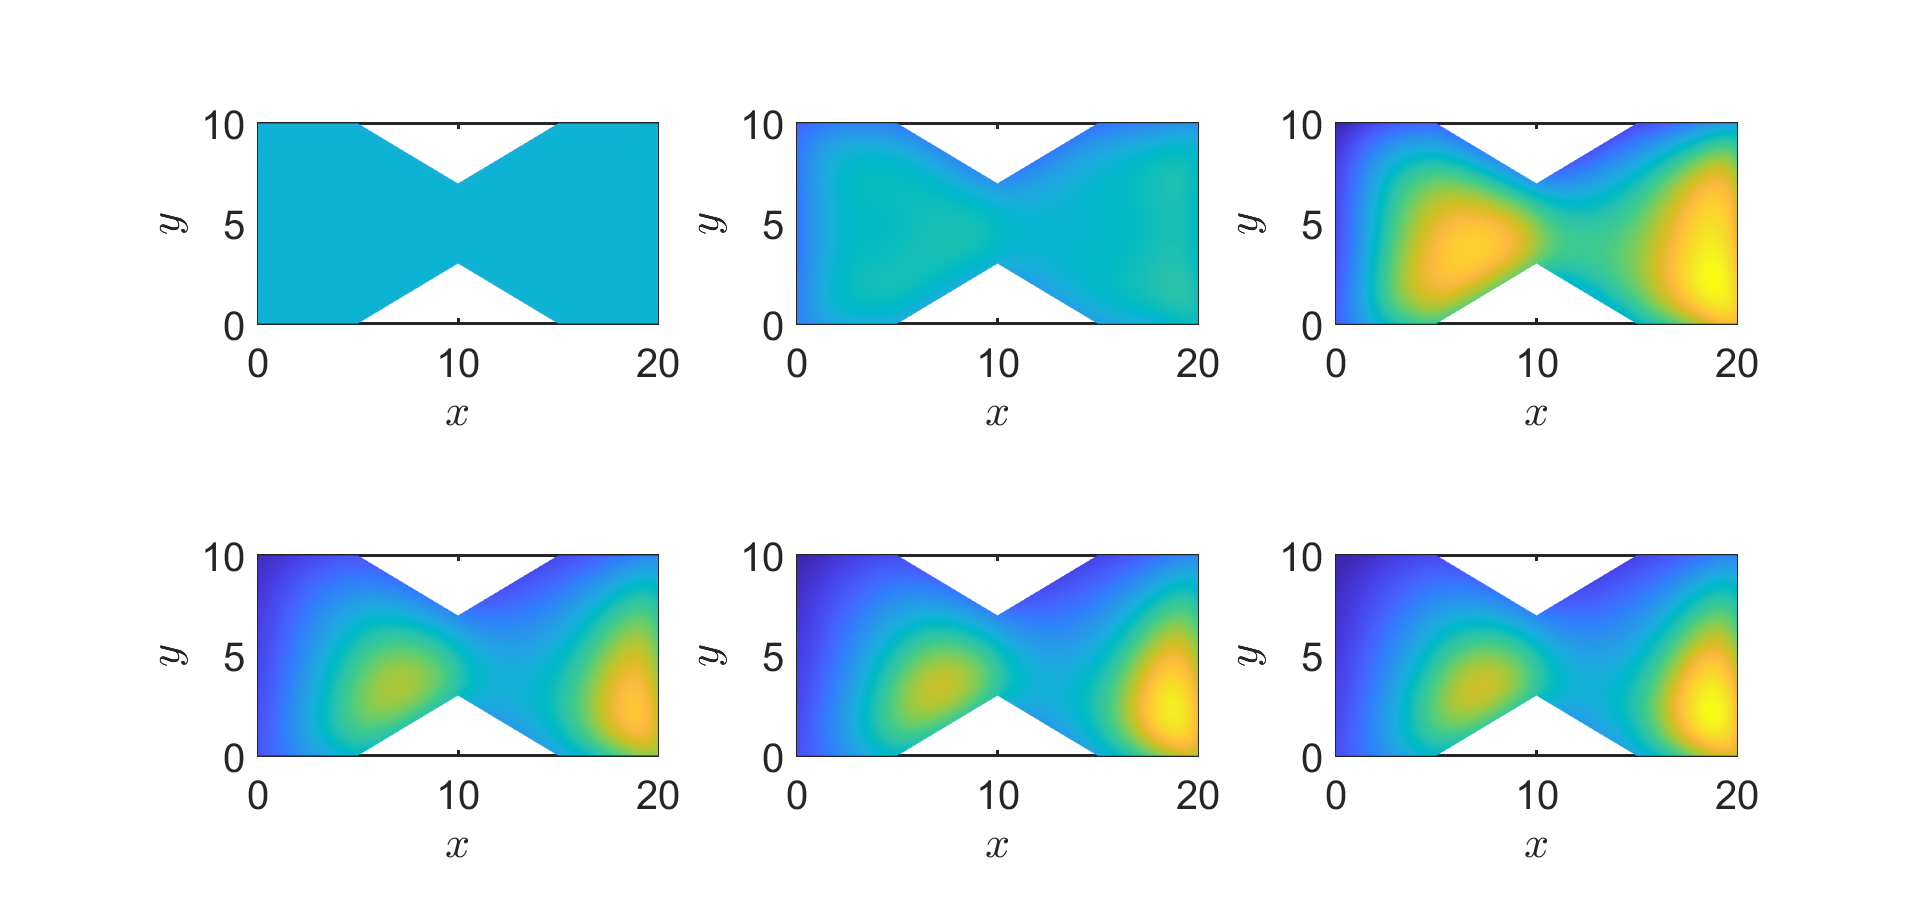
\includegraphics[scale=0.35]{MultiOpt3.png}
	\caption{Multishape Example 3: Optimal $\rho$} 
	\label{FM3a}
\end{figure}
\begin{figure}[h]
	\centering
	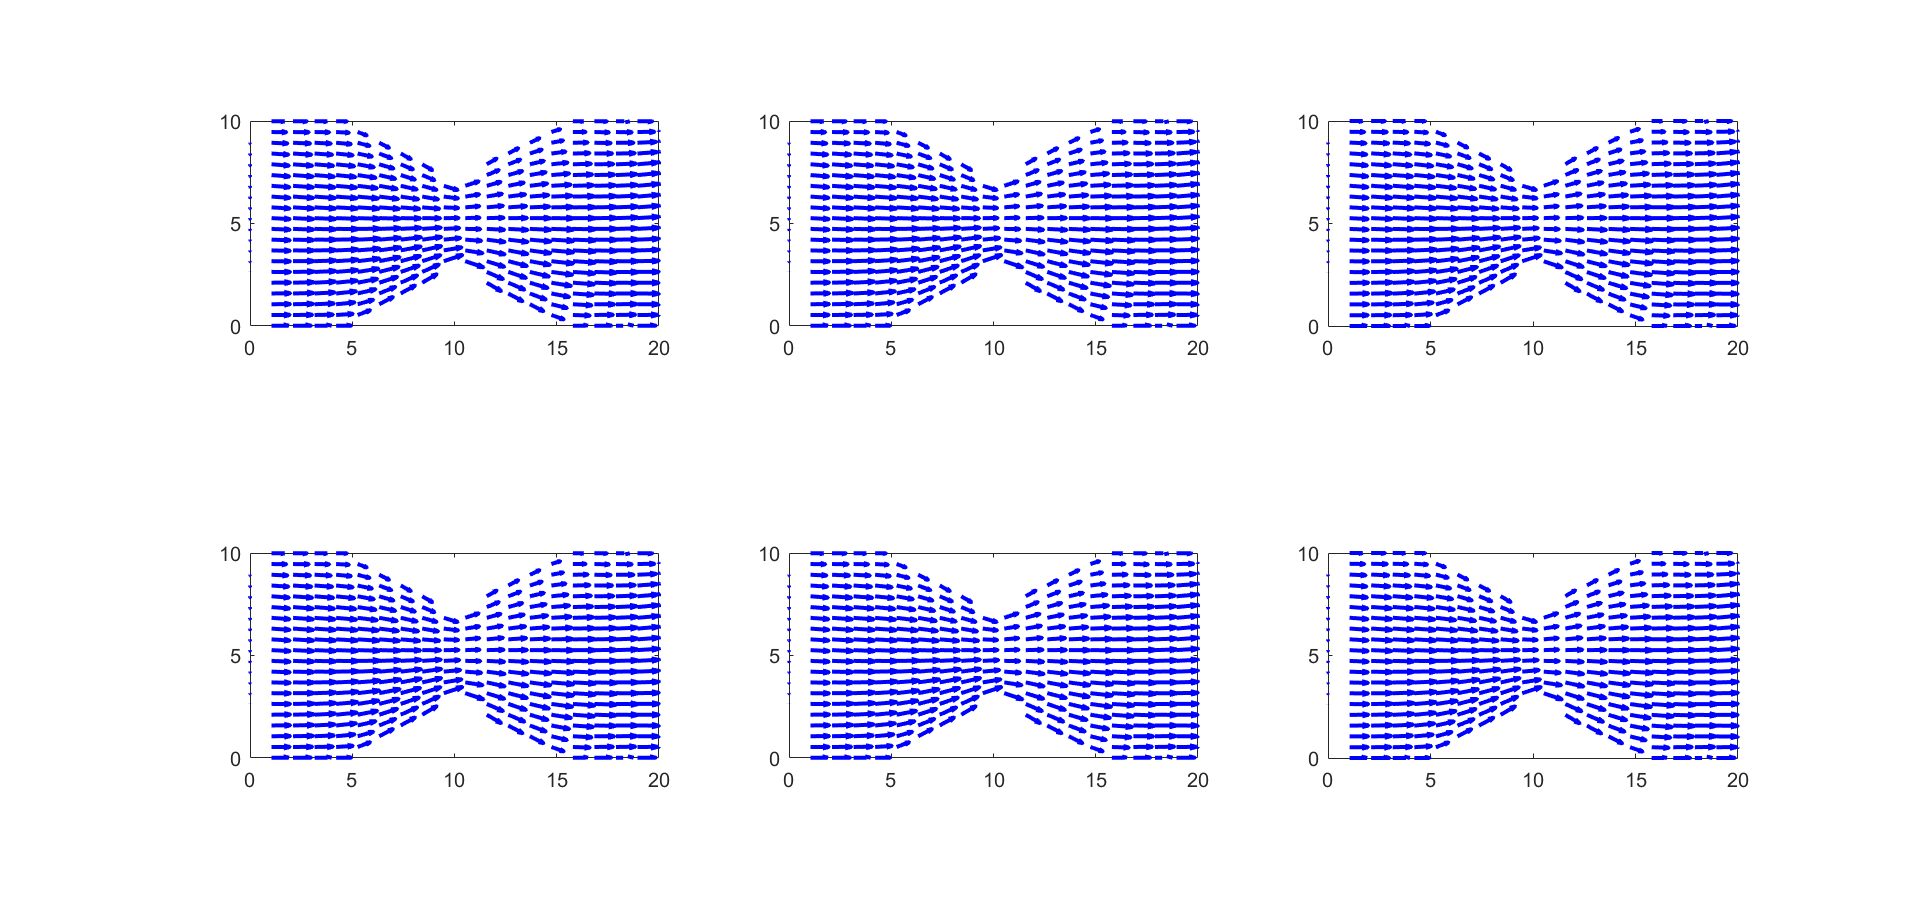
\includegraphics[scale=0.35]{MultiCont3.png}
	\caption{Multishape Example 3: Optimal control} 
	\label{FM3b}
\end{figure}
\subsubsection{Optimization in a Multishape - Time-Independent Control}
We use the first multishape example from the previous section with two quadrilaterals with the same setup and parameter choice. Here, since this is a more difficult problem, we choose $\lambda = 0.001$, which takes considerably more iterations than problems with larger $\lambda$.
We get $J_{FW} = 0.0713$ and $J_{Opt} = 0.0081$ and the result can be seen in Figures \ref{FM1} and \ref{FM2}. If we compare with the time dependent case, as expected for the time independent control, the optimal cost is higher.



\begin{figure}[h]
	\centering
	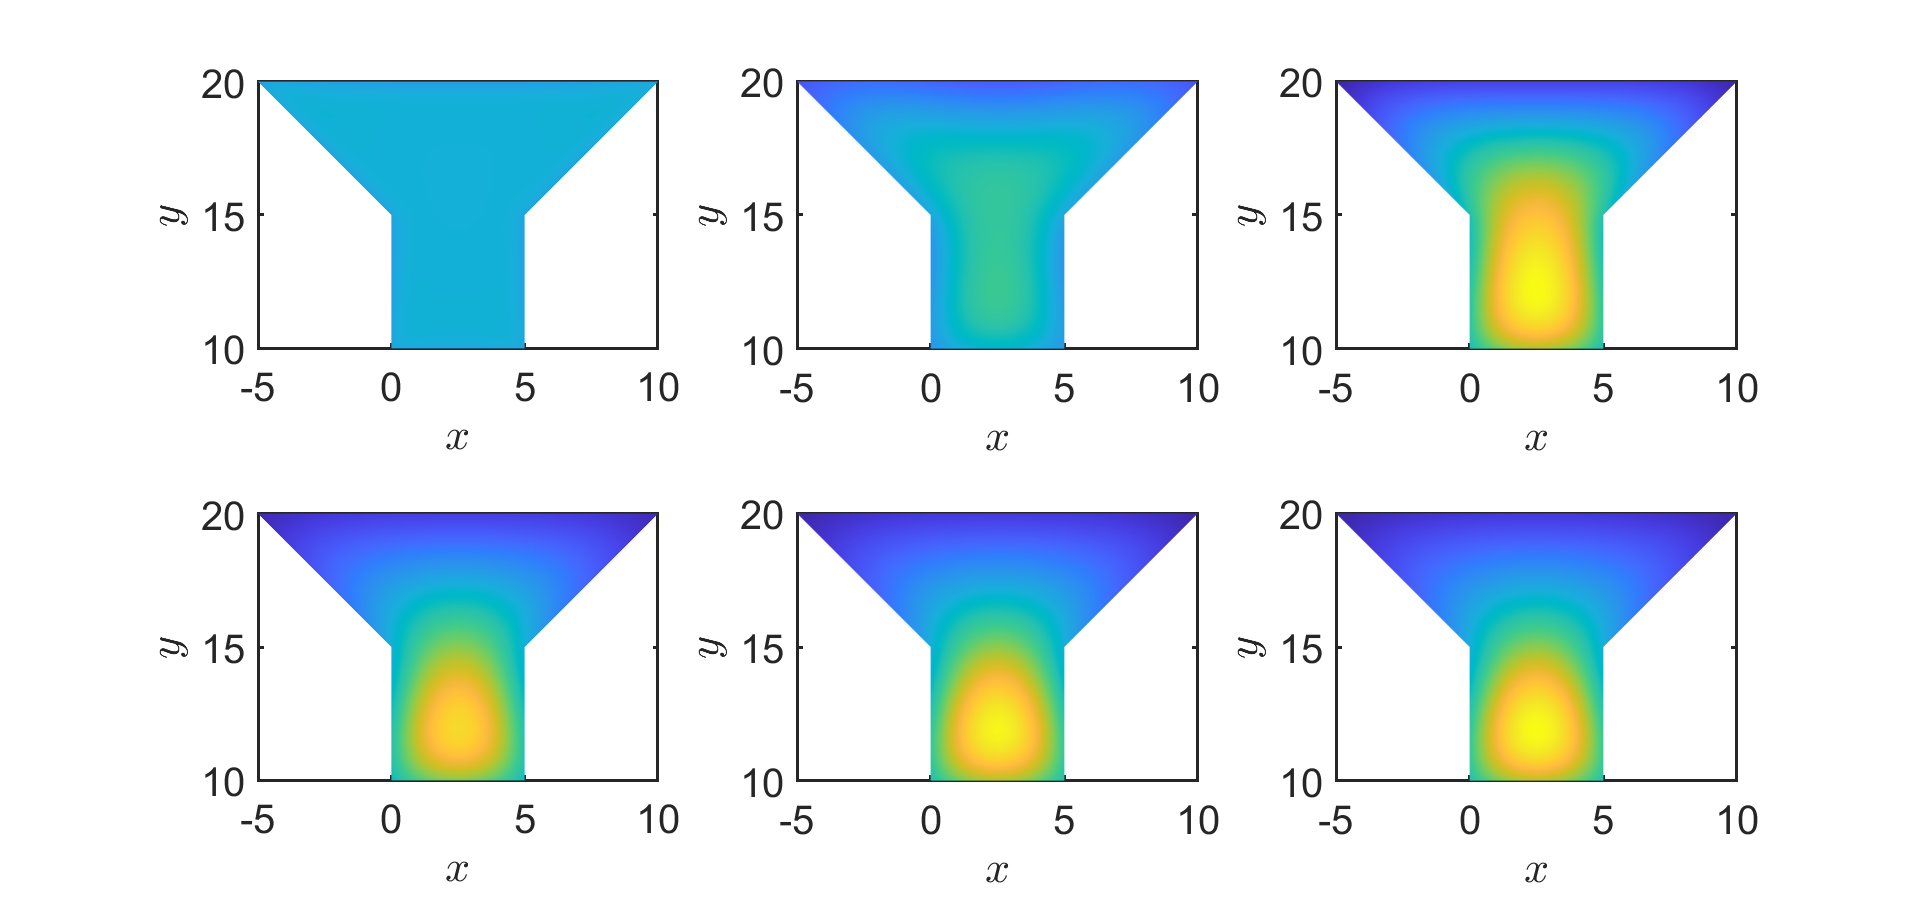
\includegraphics[scale=0.35]{MultiOpt1.png}
	\caption{Multishape Example 1 (time independent control): Optimal $\rho$} 
	\label{FM1}
\end{figure}
\begin{figure}[h]
	\centering
	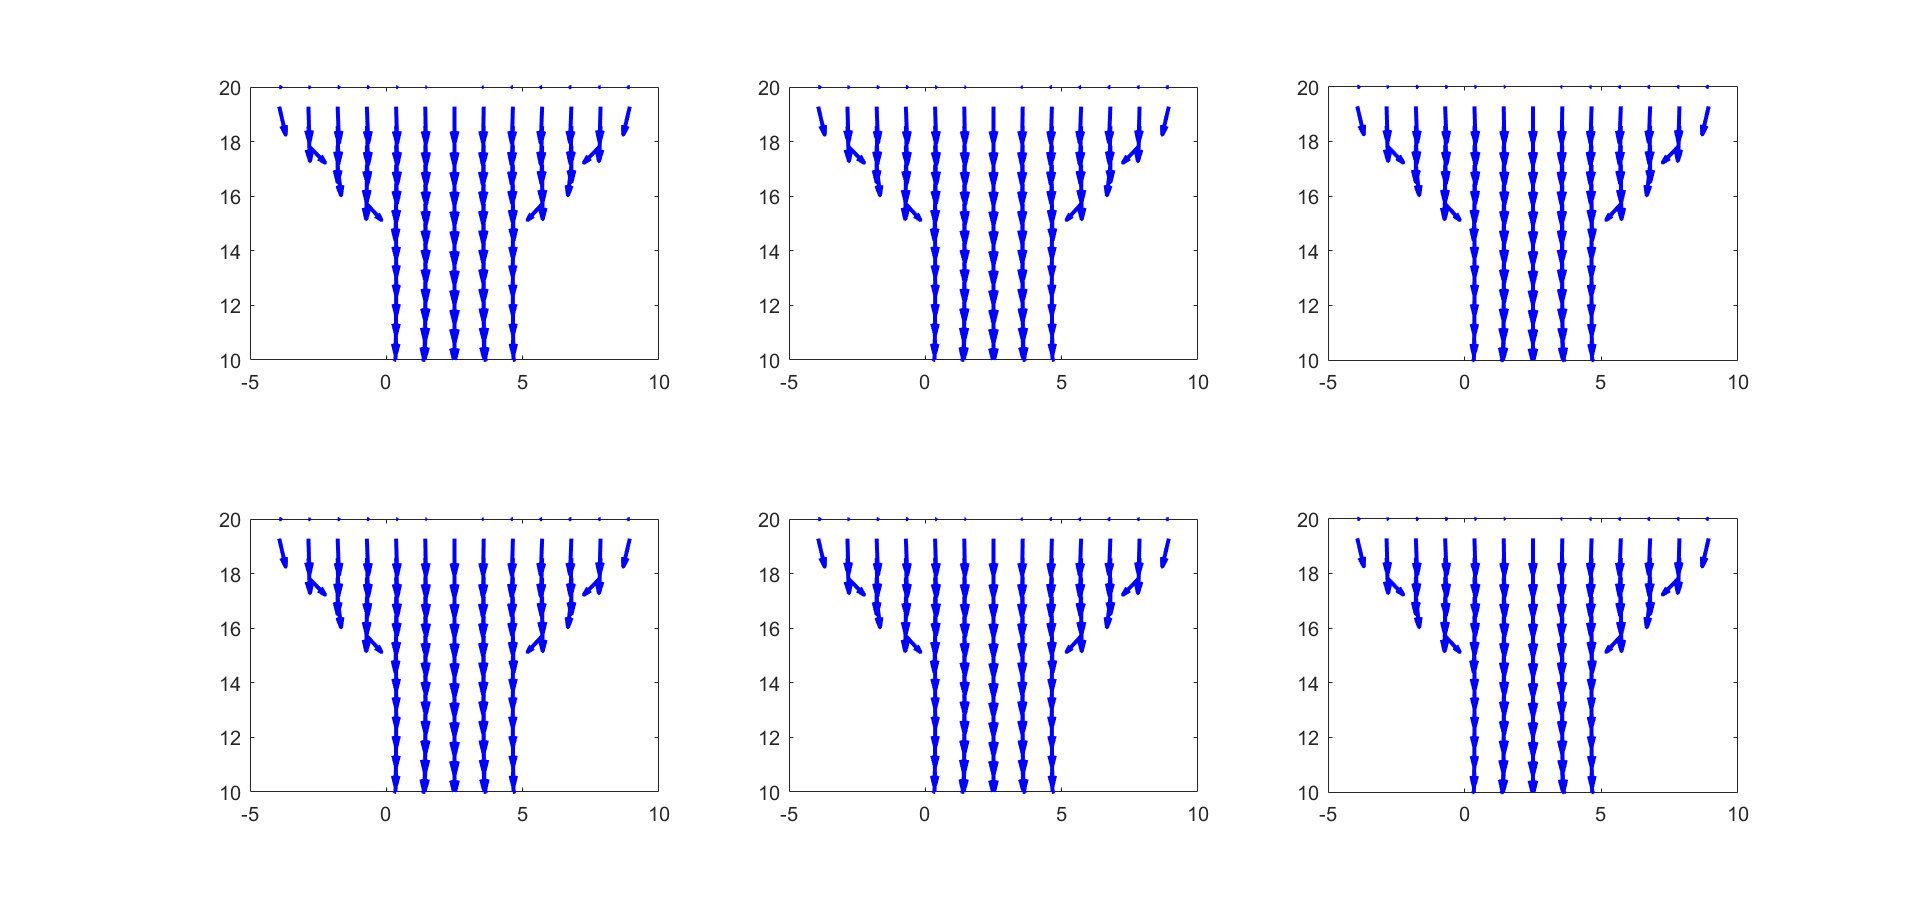
\includegraphics[scale=0.35]{MultiCont1.png}
	\caption{Multishape Example 1 (time independent control): Optimal control} 
	\label{FM2}
\end{figure}




	
	\pagebreak	
	\bibliography{GeneralBib}
	\bibliographystyle{unsrt}
	
\end{document}